\documentclass[11pt]{article}

    \usepackage[breakable]{tcolorbox}
    \usepackage{parskip} % Stop auto-indenting (to mimic markdown behaviour)
    
    \usepackage{iftex}
    \ifPDFTeX
    	\usepackage[T1]{fontenc}
    	\usepackage{mathpazo}
    \else
    	\usepackage{fontspec}
    \fi

    % Basic figure setup, for now with no caption control since it's done
    % automatically by Pandoc (which extracts ![](path) syntax from Markdown).
    \usepackage{graphicx}
    % Maintain compatibility with old templates. Remove in nbconvert 6.0
    \let\Oldincludegraphics\includegraphics


    \usepackage{caption}
    \usepackage{subcaption}


    \usepackage{float}
    \floatplacement{figure}{H} % forces figures to be placed at the correct location
    \usepackage{xcolor} % Allow colors to be defined
    \usepackage{enumerate} % Needed for markdown enumerations to work
    \usepackage{geometry} % Used to adjust the document margins
    \usepackage{amsmath} % Equations
    \usepackage{amssymb} % Equations
    \usepackage{textcomp} % defines textquotesingle
    % Hack from http://tex.stackexchange.com/a/47451/13684:
    \AtBeginDocument{%
        \def\PYZsq{\textquotesingle}% Upright quotes in Pygmentized code
    }
    \usepackage{upquote} % Upright quotes for verbatim code
    \usepackage{eurosym} % defines \euro
    \usepackage[mathletters]{ucs} % Extended unicode (utf-8) support
    \usepackage{fancyvrb} % verbatim replacement that allows latex
    \usepackage{grffile} % extends the file name processing of package graphics 
                         % to support a larger range
    \makeatletter % fix for old versions of grffile with XeLaTeX
    \@ifpackagelater{grffile}{2019/11/01}
    {
      % Do nothing on new versions
    }
    {
      \def\Gread@@xetex#1{%
        \IfFileExists{"\Gin@base".bb}%
        {\Gread@eps{\Gin@base.bb}}%
        {\Gread@@xetex@aux#1}%
      }
    }
    \makeatother
    \usepackage[Export]{adjustbox} % Used to constrain images to a maximum size
    \adjustboxset{max size={0.9\linewidth}{0.9\paperheight}}

    % The hyperref package gives us a pdf with properly built
    % internal navigation ('pdf bookmarks' for the table of contents,
    % internal cross-reference links, web links for URLs, etc.)
    \usepackage{hyperref}
    % The default LaTeX title has an obnoxious amount of whitespace. By default,
    % titling removes some of it. It also provides customization options.
    \usepackage{titling}
    \usepackage{longtable} % longtable support required by pandoc >1.10
    \usepackage{booktabs}  % table support for pandoc > 1.12.2
    \usepackage[inline]{enumitem} % IRkernel/repr support (it uses the enumerate* environment)
    \usepackage[normalem]{ulem} % ulem is needed to support strikethroughs (\sout)
                                % normalem makes italics be italics, not underlines
    \usepackage{mathrsfs}
    

    
    % Colors for the hyperref package
    \definecolor{urlcolor}{rgb}{0,.145,.698}
    \definecolor{linkcolor}{rgb}{0,0,0}
    \definecolor{citecolor}{rgb}{.12,.54,.11}

    % ANSI colors
    \definecolor{ansi-black}{HTML}{3E424D}
    \definecolor{ansi-black-intense}{HTML}{282C36}
    \definecolor{ansi-red}{HTML}{E75C58}
    \definecolor{ansi-red-intense}{HTML}{B22B31}
    \definecolor{ansi-green}{HTML}{00A250}
    \definecolor{ansi-green-intense}{HTML}{007427}
    \definecolor{ansi-yellow}{HTML}{DDB62B}
    \definecolor{ansi-yellow-intense}{HTML}{B27D12}
    \definecolor{ansi-blue}{HTML}{208FFB}
    \definecolor{ansi-blue-intense}{HTML}{0065CA}
    \definecolor{ansi-magenta}{HTML}{D160C4}
    \definecolor{ansi-magenta-intense}{HTML}{A03196}
    \definecolor{ansi-cyan}{HTML}{60C6C8}
    \definecolor{ansi-cyan-intense}{HTML}{258F8F}
    \definecolor{ansi-white}{HTML}{C5C1B4}
    \definecolor{ansi-white-intense}{HTML}{A1A6B2}
    \definecolor{ansi-default-inverse-fg}{HTML}{FFFFFF}
    \definecolor{ansi-default-inverse-bg}{HTML}{000000}

    % common color for the border for error outputs.
    \definecolor{outerrorbackground}{HTML}{FFDFDF}

    % commands and environments needed by pandoc snippets
    % extracted from the output of `pandoc -s`
    \providecommand{\tightlist}{%
      \setlength{\itemsep}{0pt}\setlength{\parskip}{0pt}}
    \DefineVerbatimEnvironment{Highlighting}{Verbatim}{commandchars=\\\{\}}
    % Add ',fontsize=\small' for more characters per line
    \newenvironment{Shaded}{}{}
    \newcommand{\KeywordTok}[1]{\textcolor[rgb]{0.00,0.44,0.13}{\textbf{{#1}}}}
    \newcommand{\DataTypeTok}[1]{\textcolor[rgb]{0.56,0.13,0.00}{{#1}}}
    \newcommand{\DecValTok}[1]{\textcolor[rgb]{0.25,0.63,0.44}{{#1}}}
    \newcommand{\BaseNTok}[1]{\textcolor[rgb]{0.25,0.63,0.44}{{#1}}}
    \newcommand{\FloatTok}[1]{\textcolor[rgb]{0.25,0.63,0.44}{{#1}}}
    \newcommand{\CharTok}[1]{\textcolor[rgb]{0.25,0.44,0.63}{{#1}}}
    \newcommand{\StringTok}[1]{\textcolor[rgb]{0.25,0.44,0.63}{{#1}}}
    \newcommand{\CommentTok}[1]{\textcolor[rgb]{0.38,0.63,0.69}{\textit{{#1}}}}
    \newcommand{\OtherTok}[1]{\textcolor[rgb]{0.00,0.44,0.13}{{#1}}}
    \newcommand{\AlertTok}[1]{\textcolor[rgb]{1.00,0.00,0.00}{\textbf{{#1}}}}
    \newcommand{\FunctionTok}[1]{\textcolor[rgb]{0.02,0.16,0.49}{{#1}}}
    \newcommand{\RegionMarkerTok}[1]{{#1}}
    \newcommand{\ErrorTok}[1]{\textcolor[rgb]{1.00,0.00,0.00}{\textbf{{#1}}}}
    \newcommand{\NormalTok}[1]{{#1}}
    
    % Additional commands for more recent versions of Pandoc
    \newcommand{\ConstantTok}[1]{\textcolor[rgb]{0.53,0.00,0.00}{{#1}}}
    \newcommand{\SpecialCharTok}[1]{\textcolor[rgb]{0.25,0.44,0.63}{{#1}}}
    \newcommand{\VerbatimStringTok}[1]{\textcolor[rgb]{0.25,0.44,0.63}{{#1}}}
    \newcommand{\SpecialStringTok}[1]{\textcolor[rgb]{0.73,0.40,0.53}{{#1}}}
    \newcommand{\ImportTok}[1]{{#1}}
    \newcommand{\DocumentationTok}[1]{\textcolor[rgb]{0.73,0.13,0.13}{\textit{{#1}}}}
    \newcommand{\AnnotationTok}[1]{\textcolor[rgb]{0.38,0.63,0.69}{\textbf{\textit{{#1}}}}}
    \newcommand{\CommentVarTok}[1]{\textcolor[rgb]{0.38,0.63,0.69}{\textbf{\textit{{#1}}}}}
    \newcommand{\VariableTok}[1]{\textcolor[rgb]{0.10,0.09,0.49}{{#1}}}
    \newcommand{\ControlFlowTok}[1]{\textcolor[rgb]{0.00,0.44,0.13}{\textbf{{#1}}}}
    \newcommand{\OperatorTok}[1]{\textcolor[rgb]{0.40,0.40,0.40}{{#1}}}
    \newcommand{\BuiltInTok}[1]{{#1}}
    \newcommand{\ExtensionTok}[1]{{#1}}
    \newcommand{\PreprocessorTok}[1]{\textcolor[rgb]{0.74,0.48,0.00}{{#1}}}
    \newcommand{\AttributeTok}[1]{\textcolor[rgb]{0.49,0.56,0.16}{{#1}}}
    \newcommand{\InformationTok}[1]{\textcolor[rgb]{0.38,0.63,0.69}{\textbf{\textit{{#1}}}}}
    \newcommand{\WarningTok}[1]{\textcolor[rgb]{0.38,0.63,0.69}{\textbf{\textit{{#1}}}}}
    
    
    % Define a nice break command that doesn't care if a line doesn't already
    % exist.
    \def\br{\hspace*{\fill} \\* }
    % Math Jax compatibility definitions
    \def\gt{>}
    \def\lt{<}
    \let\Oldtex\TeX
    \let\Oldlatex\LaTeX
    \renewcommand{\TeX}{\textrm{\Oldtex}}
    \renewcommand{\LaTeX}{\textrm{\Oldlatex}}
    % Document parameters
    % Document title
    \title{Exoplanet Model}
    
    
    
    
    
% Pygments definitions
\makeatletter
\def\PY@reset{\let\PY@it=\relax \let\PY@bf=\relax%
    \let\PY@ul=\relax \let\PY@tc=\relax%
    \let\PY@bc=\relax \let\PY@ff=\relax}
\def\PY@tok#1{\csname PY@tok@#1\endcsname}
\def\PY@toks#1+{\ifx\relax#1\empty\else%
    \PY@tok{#1}\expandafter\PY@toks\fi}
\def\PY@do#1{\PY@bc{\PY@tc{\PY@ul{%
    \PY@it{\PY@bf{\PY@ff{#1}}}}}}}
\def\PY#1#2{\PY@reset\PY@toks#1+\relax+\PY@do{#2}}

\expandafter\def\csname PY@tok@w\endcsname{\def\PY@tc##1{\textcolor[rgb]{0.73,0.73,0.73}{##1}}}
\expandafter\def\csname PY@tok@c\endcsname{\let\PY@it=\textit\def\PY@tc##1{\textcolor[rgb]{0.25,0.50,0.50}{##1}}}
\expandafter\def\csname PY@tok@cp\endcsname{\def\PY@tc##1{\textcolor[rgb]{0.74,0.48,0.00}{##1}}}
\expandafter\def\csname PY@tok@k\endcsname{\let\PY@bf=\textbf\def\PY@tc##1{\textcolor[rgb]{0.00,0.50,0.00}{##1}}}
\expandafter\def\csname PY@tok@kp\endcsname{\def\PY@tc##1{\textcolor[rgb]{0.00,0.50,0.00}{##1}}}
\expandafter\def\csname PY@tok@kt\endcsname{\def\PY@tc##1{\textcolor[rgb]{0.69,0.00,0.25}{##1}}}
\expandafter\def\csname PY@tok@o\endcsname{\def\PY@tc##1{\textcolor[rgb]{0.40,0.40,0.40}{##1}}}
\expandafter\def\csname PY@tok@ow\endcsname{\let\PY@bf=\textbf\def\PY@tc##1{\textcolor[rgb]{0.67,0.13,1.00}{##1}}}
\expandafter\def\csname PY@tok@nb\endcsname{\def\PY@tc##1{\textcolor[rgb]{0.00,0.50,0.00}{##1}}}
\expandafter\def\csname PY@tok@nf\endcsname{\def\PY@tc##1{\textcolor[rgb]{0.00,0.00,1.00}{##1}}}
\expandafter\def\csname PY@tok@nc\endcsname{\let\PY@bf=\textbf\def\PY@tc##1{\textcolor[rgb]{0.00,0.00,1.00}{##1}}}
\expandafter\def\csname PY@tok@nn\endcsname{\let\PY@bf=\textbf\def\PY@tc##1{\textcolor[rgb]{0.00,0.00,1.00}{##1}}}
\expandafter\def\csname PY@tok@ne\endcsname{\let\PY@bf=\textbf\def\PY@tc##1{\textcolor[rgb]{0.82,0.25,0.23}{##1}}}
\expandafter\def\csname PY@tok@nv\endcsname{\def\PY@tc##1{\textcolor[rgb]{0.10,0.09,0.49}{##1}}}
\expandafter\def\csname PY@tok@no\endcsname{\def\PY@tc##1{\textcolor[rgb]{0.53,0.00,0.00}{##1}}}
\expandafter\def\csname PY@tok@nl\endcsname{\def\PY@tc##1{\textcolor[rgb]{0.63,0.63,0.00}{##1}}}
\expandafter\def\csname PY@tok@ni\endcsname{\let\PY@bf=\textbf\def\PY@tc##1{\textcolor[rgb]{0.60,0.60,0.60}{##1}}}
\expandafter\def\csname PY@tok@na\endcsname{\def\PY@tc##1{\textcolor[rgb]{0.49,0.56,0.16}{##1}}}
\expandafter\def\csname PY@tok@nt\endcsname{\let\PY@bf=\textbf\def\PY@tc##1{\textcolor[rgb]{0.00,0.50,0.00}{##1}}}
\expandafter\def\csname PY@tok@nd\endcsname{\def\PY@tc##1{\textcolor[rgb]{0.67,0.13,1.00}{##1}}}
\expandafter\def\csname PY@tok@s\endcsname{\def\PY@tc##1{\textcolor[rgb]{0.73,0.13,0.13}{##1}}}
\expandafter\def\csname PY@tok@sd\endcsname{\let\PY@it=\textit\def\PY@tc##1{\textcolor[rgb]{0.73,0.13,0.13}{##1}}}
\expandafter\def\csname PY@tok@si\endcsname{\let\PY@bf=\textbf\def\PY@tc##1{\textcolor[rgb]{0.73,0.40,0.53}{##1}}}
\expandafter\def\csname PY@tok@se\endcsname{\let\PY@bf=\textbf\def\PY@tc##1{\textcolor[rgb]{0.73,0.40,0.13}{##1}}}
\expandafter\def\csname PY@tok@sr\endcsname{\def\PY@tc##1{\textcolor[rgb]{0.73,0.40,0.53}{##1}}}
\expandafter\def\csname PY@tok@ss\endcsname{\def\PY@tc##1{\textcolor[rgb]{0.10,0.09,0.49}{##1}}}
\expandafter\def\csname PY@tok@sx\endcsname{\def\PY@tc##1{\textcolor[rgb]{0.00,0.50,0.00}{##1}}}
\expandafter\def\csname PY@tok@m\endcsname{\def\PY@tc##1{\textcolor[rgb]{0.40,0.40,0.40}{##1}}}
\expandafter\def\csname PY@tok@gh\endcsname{\let\PY@bf=\textbf\def\PY@tc##1{\textcolor[rgb]{0.00,0.00,0.50}{##1}}}
\expandafter\def\csname PY@tok@gu\endcsname{\let\PY@bf=\textbf\def\PY@tc##1{\textcolor[rgb]{0.50,0.00,0.50}{##1}}}
\expandafter\def\csname PY@tok@gd\endcsname{\def\PY@tc##1{\textcolor[rgb]{0.63,0.00,0.00}{##1}}}
\expandafter\def\csname PY@tok@gi\endcsname{\def\PY@tc##1{\textcolor[rgb]{0.00,0.63,0.00}{##1}}}
\expandafter\def\csname PY@tok@gr\endcsname{\def\PY@tc##1{\textcolor[rgb]{1.00,0.00,0.00}{##1}}}
\expandafter\def\csname PY@tok@ge\endcsname{\let\PY@it=\textit}
\expandafter\def\csname PY@tok@gs\endcsname{\let\PY@bf=\textbf}
\expandafter\def\csname PY@tok@gp\endcsname{\let\PY@bf=\textbf\def\PY@tc##1{\textcolor[rgb]{0.00,0.00,0.50}{##1}}}
\expandafter\def\csname PY@tok@go\endcsname{\def\PY@tc##1{\textcolor[rgb]{0.53,0.53,0.53}{##1}}}
\expandafter\def\csname PY@tok@gt\endcsname{\def\PY@tc##1{\textcolor[rgb]{0.00,0.27,0.87}{##1}}}
\expandafter\def\csname PY@tok@err\endcsname{\def\PY@bc##1{\setlength{\fboxsep}{0pt}\fcolorbox[rgb]{1.00,0.00,0.00}{1,1,1}{\strut ##1}}}
\expandafter\def\csname PY@tok@kc\endcsname{\let\PY@bf=\textbf\def\PY@tc##1{\textcolor[rgb]{0.00,0.50,0.00}{##1}}}
\expandafter\def\csname PY@tok@kd\endcsname{\let\PY@bf=\textbf\def\PY@tc##1{\textcolor[rgb]{0.00,0.50,0.00}{##1}}}
\expandafter\def\csname PY@tok@kn\endcsname{\let\PY@bf=\textbf\def\PY@tc##1{\textcolor[rgb]{0.00,0.50,0.00}{##1}}}
\expandafter\def\csname PY@tok@kr\endcsname{\let\PY@bf=\textbf\def\PY@tc##1{\textcolor[rgb]{0.00,0.50,0.00}{##1}}}
\expandafter\def\csname PY@tok@bp\endcsname{\def\PY@tc##1{\textcolor[rgb]{0.00,0.50,0.00}{##1}}}
\expandafter\def\csname PY@tok@fm\endcsname{\def\PY@tc##1{\textcolor[rgb]{0.00,0.00,1.00}{##1}}}
\expandafter\def\csname PY@tok@vc\endcsname{\def\PY@tc##1{\textcolor[rgb]{0.10,0.09,0.49}{##1}}}
\expandafter\def\csname PY@tok@vg\endcsname{\def\PY@tc##1{\textcolor[rgb]{0.10,0.09,0.49}{##1}}}
\expandafter\def\csname PY@tok@vi\endcsname{\def\PY@tc##1{\textcolor[rgb]{0.10,0.09,0.49}{##1}}}
\expandafter\def\csname PY@tok@vm\endcsname{\def\PY@tc##1{\textcolor[rgb]{0.10,0.09,0.49}{##1}}}
\expandafter\def\csname PY@tok@sa\endcsname{\def\PY@tc##1{\textcolor[rgb]{0.73,0.13,0.13}{##1}}}
\expandafter\def\csname PY@tok@sb\endcsname{\def\PY@tc##1{\textcolor[rgb]{0.73,0.13,0.13}{##1}}}
\expandafter\def\csname PY@tok@sc\endcsname{\def\PY@tc##1{\textcolor[rgb]{0.73,0.13,0.13}{##1}}}
\expandafter\def\csname PY@tok@dl\endcsname{\def\PY@tc##1{\textcolor[rgb]{0.73,0.13,0.13}{##1}}}
\expandafter\def\csname PY@tok@s2\endcsname{\def\PY@tc##1{\textcolor[rgb]{0.73,0.13,0.13}{##1}}}
\expandafter\def\csname PY@tok@sh\endcsname{\def\PY@tc##1{\textcolor[rgb]{0.73,0.13,0.13}{##1}}}
\expandafter\def\csname PY@tok@s1\endcsname{\def\PY@tc##1{\textcolor[rgb]{0.73,0.13,0.13}{##1}}}
\expandafter\def\csname PY@tok@mb\endcsname{\def\PY@tc##1{\textcolor[rgb]{0.40,0.40,0.40}{##1}}}
\expandafter\def\csname PY@tok@mf\endcsname{\def\PY@tc##1{\textcolor[rgb]{0.40,0.40,0.40}{##1}}}
\expandafter\def\csname PY@tok@mh\endcsname{\def\PY@tc##1{\textcolor[rgb]{0.40,0.40,0.40}{##1}}}
\expandafter\def\csname PY@tok@mi\endcsname{\def\PY@tc##1{\textcolor[rgb]{0.40,0.40,0.40}{##1}}}
\expandafter\def\csname PY@tok@il\endcsname{\def\PY@tc##1{\textcolor[rgb]{0.40,0.40,0.40}{##1}}}
\expandafter\def\csname PY@tok@mo\endcsname{\def\PY@tc##1{\textcolor[rgb]{0.40,0.40,0.40}{##1}}}
\expandafter\def\csname PY@tok@ch\endcsname{\let\PY@it=\textit\def\PY@tc##1{\textcolor[rgb]{0.25,0.50,0.50}{##1}}}
\expandafter\def\csname PY@tok@cm\endcsname{\let\PY@it=\textit\def\PY@tc##1{\textcolor[rgb]{0.25,0.50,0.50}{##1}}}
\expandafter\def\csname PY@tok@cpf\endcsname{\let\PY@it=\textit\def\PY@tc##1{\textcolor[rgb]{0.25,0.50,0.50}{##1}}}
\expandafter\def\csname PY@tok@c1\endcsname{\let\PY@it=\textit\def\PY@tc##1{\textcolor[rgb]{0.25,0.50,0.50}{##1}}}
\expandafter\def\csname PY@tok@cs\endcsname{\let\PY@it=\textit\def\PY@tc##1{\textcolor[rgb]{0.25,0.50,0.50}{##1}}}

\def\PYZbs{\char`\\}
\def\PYZus{\char`\_}
\def\PYZob{\char`\{}
\def\PYZcb{\char`\}}
\def\PYZca{\char`\^}
\def\PYZam{\char`\&}
\def\PYZlt{\char`\<}
\def\PYZgt{\char`\>}
\def\PYZsh{\char`\#}
\def\PYZpc{\char`\%}
\def\PYZdl{\char`\$}
\def\PYZhy{\char`\-}
\def\PYZsq{\char`\'}
\def\PYZdq{\char`\"}
\def\PYZti{\char`\~}
% for compatibility with earlier versions
\def\PYZat{@}
\def\PYZlb{[}
\def\PYZrb{]}
\makeatother


    % For linebreaks inside Verbatim environment from package fancyvrb. 
    \makeatletter
        \newbox\Wrappedcontinuationbox 
        \newbox\Wrappedvisiblespacebox 
        \newcommand*\Wrappedvisiblespace {\textcolor{red}{\textvisiblespace}} 
        \newcommand*\Wrappedcontinuationsymbol {\textcolor{red}{\llap{\tiny$\m@th\hookrightarrow$}}} 
        \newcommand*\Wrappedcontinuationindent {3ex } 
        \newcommand*\Wrappedafterbreak {\kern\Wrappedcontinuationindent\copy\Wrappedcontinuationbox} 
        % Take advantage of the already applied Pygments mark-up to insert 
        % potential linebreaks for TeX processing. 
        %        {, <, #, %, $, ' and ": go to next line. 
        %        _, }, ^, &, >, - and ~: stay at end of broken line. 
        % Use of \textquotesingle for straight quote. 
        \newcommand*\Wrappedbreaksatspecials {% 
            \def\PYGZus{\discretionary{\char`\_}{\Wrappedafterbreak}{\char`\_}}% 
            \def\PYGZob{\discretionary{}{\Wrappedafterbreak\char`\{}{\char`\{}}% 
            \def\PYGZcb{\discretionary{\char`\}}{\Wrappedafterbreak}{\char`\}}}% 
            \def\PYGZca{\discretionary{\char`\^}{\Wrappedafterbreak}{\char`\^}}% 
            \def\PYGZam{\discretionary{\char`\&}{\Wrappedafterbreak}{\char`\&}}% 
            \def\PYGZlt{\discretionary{}{\Wrappedafterbreak\char`\<}{\char`\<}}% 
            \def\PYGZgt{\discretionary{\char`\>}{\Wrappedafterbreak}{\char`\>}}% 
            \def\PYGZsh{\discretionary{}{\Wrappedafterbreak\char`\#}{\char`\#}}% 
            \def\PYGZpc{\discretionary{}{\Wrappedafterbreak\char`\%}{\char`\%}}% 
            \def\PYGZdl{\discretionary{}{\Wrappedafterbreak\char`\$}{\char`\$}}% 
            \def\PYGZhy{\discretionary{\char`\-}{\Wrappedafterbreak}{\char`\-}}% 
            \def\PYGZsq{\discretionary{}{\Wrappedafterbreak\textquotesingle}{\textquotesingle}}% 
            \def\PYGZdq{\discretionary{}{\Wrappedafterbreak\char`\"}{\char`\"}}% 
            \def\PYGZti{\discretionary{\char`\~}{\Wrappedafterbreak}{\char`\~}}% 
        } 
        % Some characters . , ; ? ! / are not pygmentized. 
        % This macro makes them "active" and they will insert potential linebreaks 
        \newcommand*\Wrappedbreaksatpunct {% 
            \lccode`\~`\.\lowercase{\def~}{\discretionary{\hbox{\char`\.}}{\Wrappedafterbreak}{\hbox{\char`\.}}}% 
            \lccode`\~`\,\lowercase{\def~}{\discretionary{\hbox{\char`\,}}{\Wrappedafterbreak}{\hbox{\char`\,}}}% 
            \lccode`\~`\;\lowercase{\def~}{\discretionary{\hbox{\char`\;}}{\Wrappedafterbreak}{\hbox{\char`\;}}}% 
            \lccode`\~`\:\lowercase{\def~}{\discretionary{\hbox{\char`\:}}{\Wrappedafterbreak}{\hbox{\char`\:}}}% 
            \lccode`\~`\?\lowercase{\def~}{\discretionary{\hbox{\char`\?}}{\Wrappedafterbreak}{\hbox{\char`\?}}}% 
            \lccode`\~`\!\lowercase{\def~}{\discretionary{\hbox{\char`\!}}{\Wrappedafterbreak}{\hbox{\char`\!}}}% 
            \lccode`\~`\/\lowercase{\def~}{\discretionary{\hbox{\char`\/}}{\Wrappedafterbreak}{\hbox{\char`\/}}}% 
            \catcode`\.\active
            \catcode`\,\active 
            \catcode`\;\active
            \catcode`\:\active
            \catcode`\?\active
            \catcode`\!\active
            \catcode`\/\active 
            \lccode`\~`\~ 	
        }
    \makeatother

    \let\OriginalVerbatim=\Verbatim
    \makeatletter
    \renewcommand{\Verbatim}[1][1]{%
        %\parskip\z@skip
        \sbox\Wrappedcontinuationbox {\Wrappedcontinuationsymbol}%
        \sbox\Wrappedvisiblespacebox {\FV@SetupFont\Wrappedvisiblespace}%
        \def\FancyVerbFormatLine ##1{\hsize\linewidth
            \vtop{\raggedright\hyphenpenalty\z@\exhyphenpenalty\z@
                \doublehyphendemerits\z@\finalhyphendemerits\z@
                \strut ##1\strut}%
        }%
        % If the linebreak is at a space, the latter will be displayed as visible
        % space at end of first line, and a continuation symbol starts next line.
        % Stretch/shrink are however usually zero for typewriter font.
        \def\FV@Space {%
            \nobreak\hskip\z@ plus\fontdimen3\font minus\fontdimen4\font
            \discretionary{\copy\Wrappedvisiblespacebox}{\Wrappedafterbreak}
            {\kern\fontdimen2\font}%
        }%
        
        % Allow breaks at special characters using \PYG... macros.
        \Wrappedbreaksatspecials
        % Breaks at punctuation characters . , ; ? ! and / need catcode=\active 	
        \OriginalVerbatim[#1,codes*=\Wrappedbreaksatpunct]%
    }
    \makeatother

    % Exact colors from NB
    \definecolor{incolor}{HTML}{303F9F}
    \definecolor{outcolor}{HTML}{D84315}
    \definecolor{cellborder}{HTML}{CFCFCF}
    \definecolor{cellbackground}{HTML}{F7F7F7}
    
    % prompt
    \makeatletter
    \newcommand{\boxspacing}{\kern\kvtcb@left@rule\kern\kvtcb@boxsep}
    \makeatother
    \newcommand{\prompt}[4]{
        {\ttfamily\llap{{\color{#2}[#3]:\hspace{3pt}#4}}\vspace{-\baselineskip}}
    }
    

    
    % Prevent overflowing lines due to hard-to-break entities
    \sloppy 
    % Setup hyperref package
    \hypersetup{
      breaklinks=true,  % so long urls are correctly broken across lines
      colorlinks=true,
      urlcolor=urlcolor,
      linkcolor=linkcolor,
      citecolor=citecolor,
      }
    
    % Formatting for matplotlib graph titles. Left-aligned
    \newcommand*{\figuretitle}[1]{
    	{\textbf{#1}
    	\par\vspace{-1em}}
    }
    
    % Slightly bigger margins than the latex defaults
    \geometry{verbose,tmargin=1in,bmargin=1in,lmargin=1in,rmargin=1in}
    
    \title{Exoplanet Model}
    \author{Chenyang Li}
    \date{March 23, 2020}
	

 \begin{document}
	
	\begin{titlepage}
		\begin{center}
			\vspace*{1cm}
			
			\Huge
			\textbf{Exoplanet Model}
			
			\vspace{0.5cm}
			\LARGE
			March 23, 2020
			
			\vspace{1.5cm}
			
			\textbf{Chenyang Li}
			
			\vfill
			
			
			
\includegraphics[width=0.15\textwidth]{crest}
			
			\vspace{0.8cm}
			
			\hypertarget{eton-college-computational-physics-prize-2020}{%
			\section*{Eton College Computational Physics Prize 2020}\label{eton-college-computational-physics-prize-2020}}
			
			
		\end{center}
	\end{titlepage}
	


	\pagebreak
	\begingroup % start a TeX group
	\color{black}% or whatever color you wish to use
	\tableofcontents
	\endgroup
	\pagebreak


    \maketitle
    \begin{center}\rule{0.5\linewidth}{0.5pt}\end{center}
    
    \hypertarget{introduction}{%
\section{Introduction}\label{introduction}}


\hypertarget{historical-searches-for-exoplanets}{%
\subsection{Historical Searches for Exoplanets}\label{historical-searches-for-exoplanets}}

Since antiquity, the question concerning the existence of worlds apart
from our own has always been of significant theoretical interest, with
views ranging from Aristotle's rather forceful assertion that ``it is
clear that the earth does not move, and that it does not lie elsewhere
than at the centre'' to Italian philosopher Giordano Bruno's claim that
``this space we declare to be infinite {[}\ldots{]} In it are an
infinity of worlds of the same kind as our own.''

While the philosophical debate continued, it was not until Galileo's
discovery of Jupiter's moons when the possibility of the existence of
exoplanets truly presented themselves to the early scientific community.
Over three hundred years later, in 1992, Wolszczan and Frail announced
the discovery of two rocky planets orbiting PSR B1 257+12, a pulsar in
the constellation Virgo. As the result of several improvements in
instrumentation and observing techniques, in the past two decades the
number of exoplanets discovered has dramatically increased: as of
February, 2020, over \href{http://exoplanet.eu/catalog/}{4000} have been
found (Schneider, 2020).

    \hypertarget{exoplanet-detection-methods}{%
\subsection{Exoplanet Detection Methods}\label{exoplanet-detection-methods}}

Several methods for the discovery of exoplanets are currently in use,
with multiple proposed methods still yet to detect an exoplanet. The
main difficulty arises due to the fact that exoplanets are extremely dim
when compared to the parent star, making direct imaging very difficult
and only applicable to a small number of cases.

\hypertarget{methods-discussed-in-this-article}{%
\paragraph{Methods Discussed in this Article:}\label{methods-discussed-in-this-article}}

\hypertarget{radial-velocity}{%
\paragraph{Radial Velocity}\label{radial-velocity}}

Clearest when the planetary system is seen side on, this method detects
the Doppler shift of the spectral lines of the starlight, caused by the
gravitational pull of an orbiting companion planet. The mass of the
planet can be calculated from the variations in radial velocity it
causes on its parent star.

\hypertarget{transits}{%
\paragraph{Transits}\label{transits}}

Used exclusively for side on orbits, this method detects the periodic
dip in light intensity caused by the planet passing in front of its
parent star and blocking some of the emitted light, producing a light
curve. Note that this event is called a transit, whereas the passage of
the planet behind its parent star is called an occultation or sometimes
a secondary eclipse. For a transiting object to be confirmed as a
planet, its mass needs to be measured through the radial velocity
method. The transit method is most sensitive to large planets with a
small orbital semi-major axis such as a \emph{Hot Jupiter}, where the
probability of observing their transits is greater.

\quad
\begin{figure}[!ht]
	\centering
	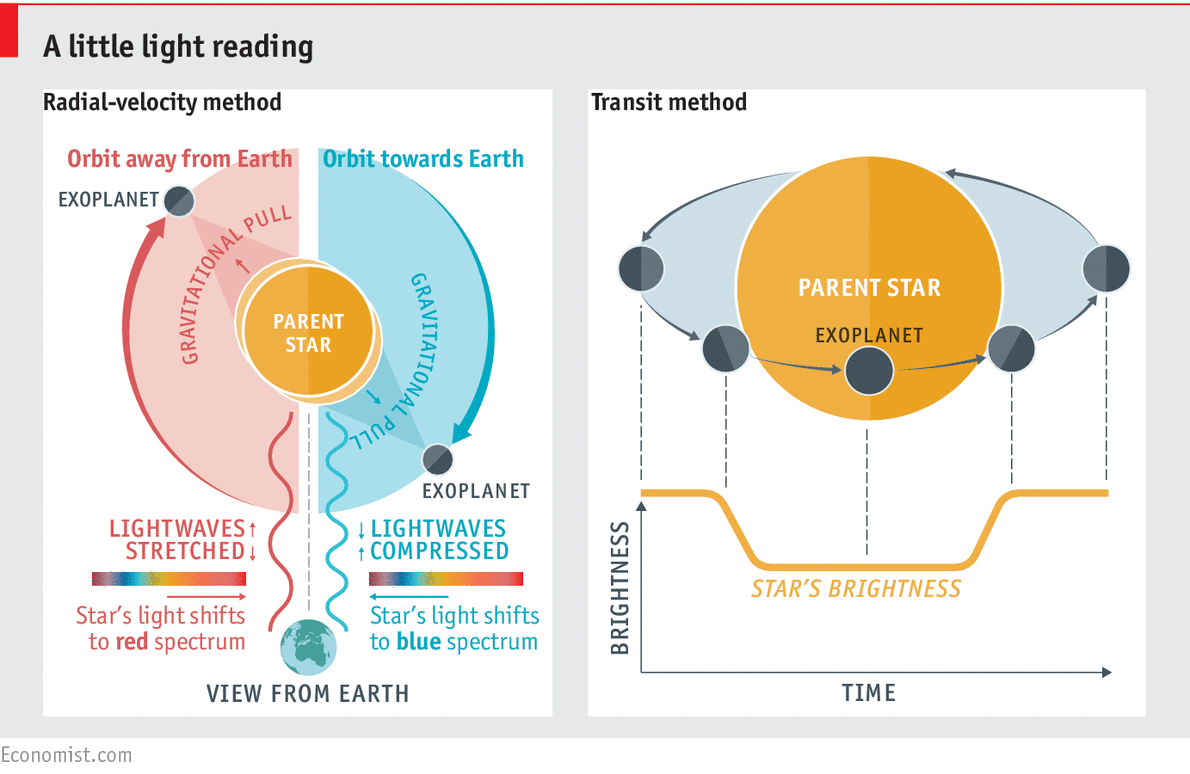
\includegraphics[width=0.8\textwidth]{../images/methods.png}
	\caption{The radial velocity and transit methods (Economist, 2016).} \label{Figure 1.a}
\end{figure}


\hypertarget{other-methods}{%
\subsection{Other Methods}\label{other-methods}}

\hypertarget{astrometry}{%
\paragraph{Astrometry}\label{astrometry}}

This refers to the accurate measurement of the positions of the star.
Most effective for finding high-mass planets in wide orbits around
nearby relatively low-mass stars, wobbles detected in the star's
position caused by the gravitational pull of the exoplanet can be used
to indirectly detect planets.

\hypertarget{gravitational-microlensing}{%
\paragraph{Gravitational Microlensing}\label{gravitational-microlensing}}

Requiring a crowed stellar background, this method detects the
magnification of a background star due to the deflection of its light by
the gravitational field of a foreground planetary system acting as a
gravitational lens. Whilst the parent star acts as the main lens, the
orbiting planet adds a much briefer magnification effect in addition to
the lensing of its host star. The microlensing technique is sensitive to
down to Earth sized exoplanets, although the detection of small planets
depends on the time sampling, as the smaller the planet, the shorter the
microlensing event.

\hypertarget{direct-imaging}{%
\paragraph{Direct Imaging}\label{direct-imaging}}

Detecting the light emitted or reflected from a planet itself, direct
imaging only works for a minority of planets that are far enough from
their parent stars so that the stellar glare can be suppressed. A
chronograph or an interferometer can be used to suppress light emitted
from the star. The direct imaging technique uses adaptive optics to
sharpen the image of the star which is then easier to suppress, and to
sharpen the image of the planet which is then easier to detect.

\hypertarget{pulsar-timing}{%
\paragraph{Pulsar Timing}\label{pulsar-timing}}

This method detects regular anomalies in the frequency of the radio
pulses of a neutron star; an Earth-like planet around a pulsar creates a
detectable pulse delay of 1.2 milliseconds. As the name suggests, this
method is limited to pulsars.

\quad
\begin{figure}[!ht]
	\centering 
	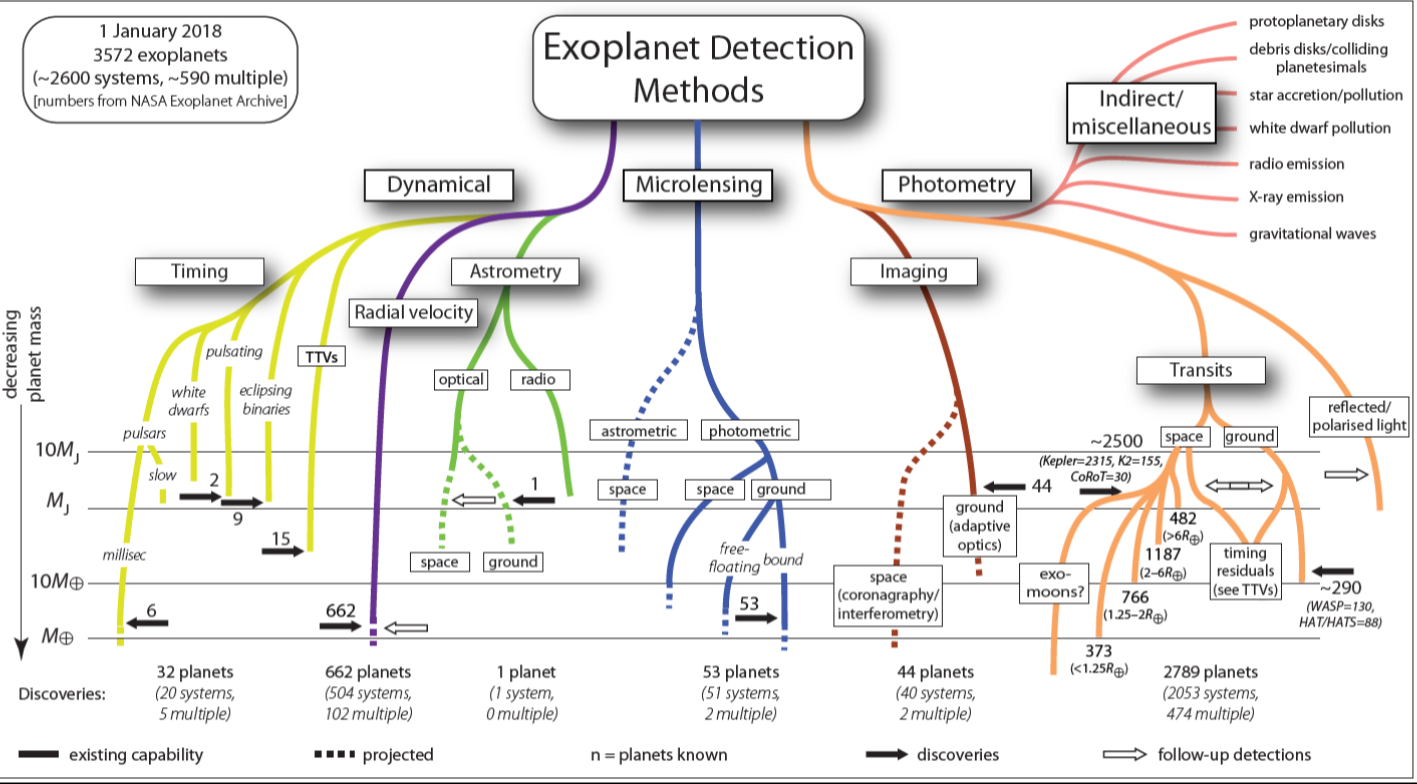
\includegraphics[width=0.9\textwidth]{../images/Detection.png}
	\caption{A comprehensive summary of the different methods for detecting
		exoplanets, as well as the total number of planetary systems found per
		method as of 1 January 2018 (Perryman, 2018).} \label{Figure 1.b}
\end{figure}


\begin{center}\rule{0.5\linewidth}{0.5pt}\end{center}

    \hypertarget{project-overview}{%
\section{Project Overview}\label{project-overview}}


\hypertarget{fundamental-aims}{%
\subsection{Fundamental Aims}\label{fundamental-aims}}

Inspired by the awarding of the Nobel Prize in Physics (2019) to Mayor
and Queloz for the discovery of exoplanets using the radial velocity
method, in this project, we aim to model a two-body exoplanet system,
applying Kepler's laws to given orbital parameters in order to
accurately predict the movement of both the planet and parent star. From
there both the light curve and radial velocity readings will be
extrapolated, using the exact analytic formulae for the eclipse of a
star described by quadratic limb darkening, and Kepler's equation with
the equation for radial velocity variations.

\hypertarget{flow-summary}{%
\subsection{Flow Summary}\label{flow-summary}}

The algorithmic flow can be summarised as follows: 
\begin{enumerate}
	\item Select a desired binary star system.
	\item Load the orbital elements of that desired system (see \ref{orbital-elements}) 
	\item Compute the mean anomaly from \(M = \frac{2\pi}{P}(t-T)\), where \(P\) is the orbital period of the planet and \(T\) is the time of last passage at periaston.
	\item Use Newton's method to solve Kepler's equation \(M =E - e\sin(E)\), deriving \(E\), the eccentric anomaly. 
	\item From \(E\) derive \(d\), the side on centre-to-centre distance between the planet and star. 
	\item Calculate \(\nu\), the true anomaly. 
	\item From \(d\), integrate the unobstructed flux emitted from the parent star. 
	\item Integrate to solve for the total flux emitted, using the light intensity equation described by quadratic limb darkening (Mandel and Agol, 2002). 
	\item Derive \(V\), the observed radial velocity variations, from \(\nu\). 
	\item Repeat steps 2-9 for each timestamp of the period of the orbit, producing two arrays of results that can be plotted against the	timestamp.
\end{enumerate}

    \hypertarget{orbital-elements}{%
\subsection{Orbital Elements}\label{orbital-elements}}

As the parameters which are required to uniquely define a particular
orbit, orbital elements are essential for mathematically modelling a
Kepler orbit; note that, while sufficiently accurate for the purposes of
this project, real orbits change over time due to gravitational
perturbations by other objects and the effects of relativity. A
Keplerian orbit is merely an idealized approximation at a given time.

Whilst there may be different ways to describe an orbit, in general the
following parameters are used: 

\begin{itemize}
	\item \(t_{0}\): The time of a reference transit for each orbit.
	\item \(a\): semi-major axis.
	\item \(b\): impact parameters of the orbit.
	\item \(e\): eccentricity of the orbit, describing how elongated the ellipse is.
	\item \(\omega\): argument of periapsis.
	\item \(i\): inclination of orbit.
\end{itemize}

Note that in our simulation, the period of the orbit, and the mass and
radius of both planet and star, are also used. Additionally, the
longitude of the ascending node, \(\Omega\), is not included in our
model as it is difficult to measure and does not affect the final
results.

\quad

\begin{figure}[!ht]
	\centering 
	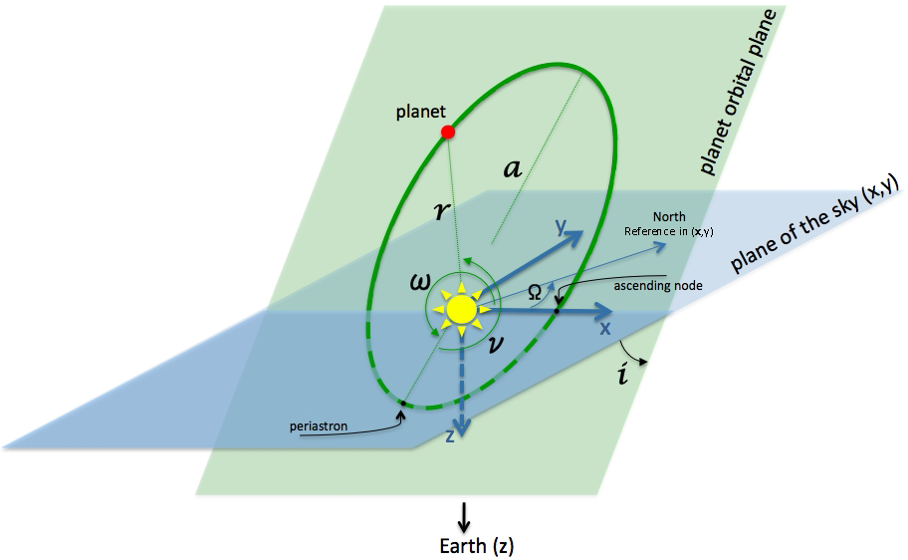
\includegraphics[width=0.75\textwidth]{../images/orbit_elements.png}
	\caption{Diagram showing orbital elements (Wikipedia, 2020a).} \label{Figure 2.a.i}
\end{figure}

\smallskip

\begin{figure}[H]
	\centering
	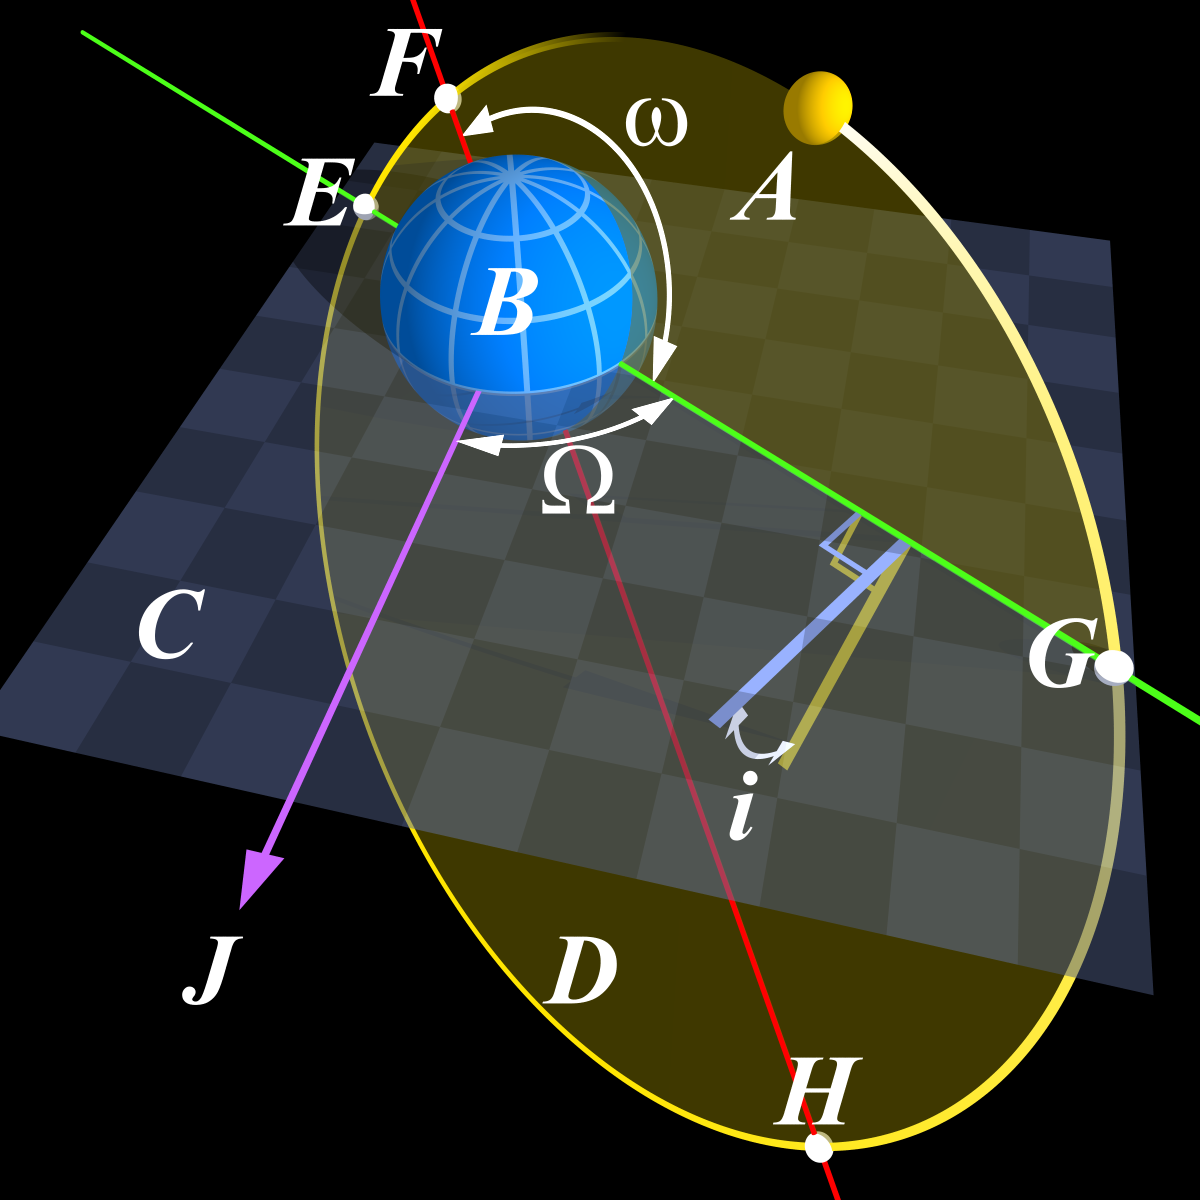
\includegraphics[width=0.4\textwidth]{../images/Angular_Parameters_of_Elliptical_Orbit.png}
	\caption{Angular parameters (Wikipedia, 2020a).} \label{Figure 2.a.ii}
\end{figure}

    \hypertarget{anomalies}{%
\subsection{Anomalies}\label{anomalies}}

In astronomy, \emph{anomaly} refers to three different angles which are used
to map the motion of the planet as it orbits a star; these are
fundamentally linked with each other through a series of equations (Reed,
2019). An excellent source on the derivation of these is found
\href{http://www.bogan.ca/orbits/kepler/e_anomly.html}{here.}

\hypertarget{mean-anomaly}{%
\subsubsection{Mean Anomaly}\label{mean-anomaly}}

This is the angle between lines drawn from the star to the periapsis and
to a point moving in the orbit at a uniform rate (on a circular orbit),
corresponding to the period of revolution of the planet.
\begin{equation*}
M = \frac{2\pi}{P}(t-T) 
\end{equation*} where \(P\) is the orbital period of the planet and
\(T\) is the time of last passage at periaston (where the planet comes
closest to the star).

This is illustrated below as Figure \ref{Figure 2.b}:

\begin{figure}[!ht]
	\centering
	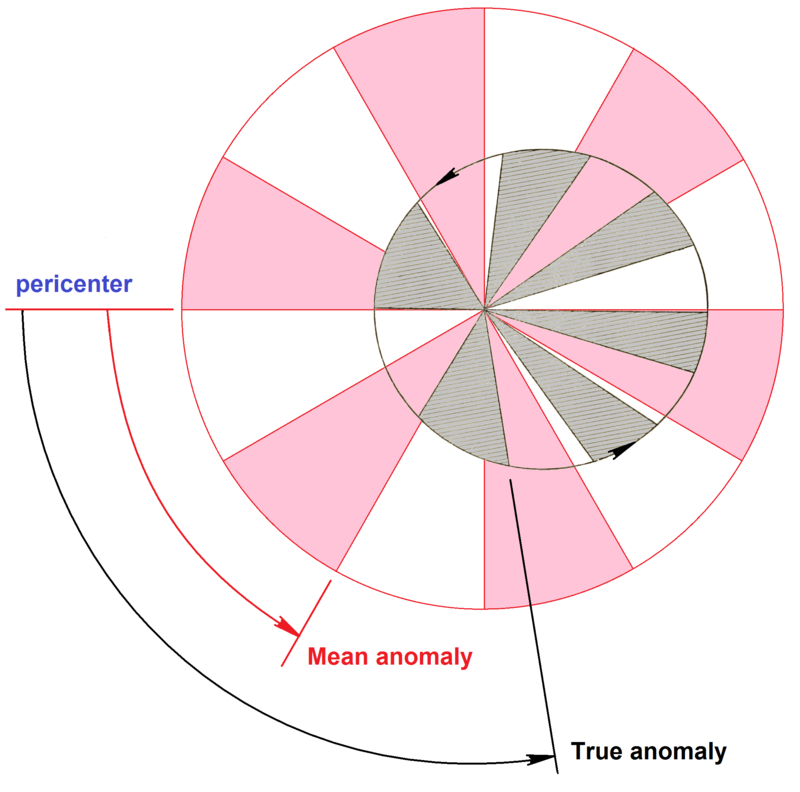
\includegraphics[width=0.4\textwidth]{../images/Mean_anomaly_diagram.png}
	\caption{``Area swept out per unit time is in grey by an object in an elliptical orbit, and an imaginary object in a circular orbit is in pink.'' Note that for visual simplicity, a non-overlapping circular orbit is drawn: this circular orbit with same orbital period is not shown in true scale with this elliptical orbit. For the scale to be true for orbits of equal period, the radius of circle must equal the semi-major axis of the ellipse. (Wikipedia, 2020b)} 
	
	\label{Figure 2.b}
\end{figure}

    \hypertarget{eccentric-anomaly}{%
\subsubsection{Eccentric Anomaly}\label{eccentric-anomaly}}

This is the angle \(E\), between the periapsis, the centre of the
ellipse, and the point $P'$ (shown in Figure \ref{Figure 2.c}), which is located by
drawing a perpendicular to \(CF\) passing through the planet and
intersecting a circle of \(C-\)periapsis.

The eccentric anomaly is related to the mean anomaly through the
following relationship, known as Kepler's equation:

\begin{equation*}
M = E - e\sin{E} 
\end{equation*}

This equation is known as a transcendental function as it cannot be
solved analytically; rather, it is solved numerically, using Newton's method, which consists of finding a better value at each
iteration using the value previously found at the previous iteration,
the expression of the function, and its derivative:
\(x_{n+1} = x_{n}-\frac{f(x_{n})}{f'(x_{n})}\). These two functions are
given below:

\begin{align}
E(M)  & = E - e\sin{E} - M \\
E'(M) & = 1 - e\cos{E}
\end{align}

\vfill

\hypertarget{true-anomaly}{%
\subsubsection{True Anomaly}\label{true-anomaly}}

This is the angle \(f\) in Figure \ref{Figure 2.c}, but is more commonly denoted as
\(\theta\) or \(\nu\). In this study we use \(\nu\).

The true anomaly can be derived from the eccentric anomaly through the following equation:

\begin{equation*}
\cos{\nu} = \frac{ \cos{E} - e }{ 1 - e\cos{E} } 
\end{equation*}


\begin{figure}[!ht]
	\centering
	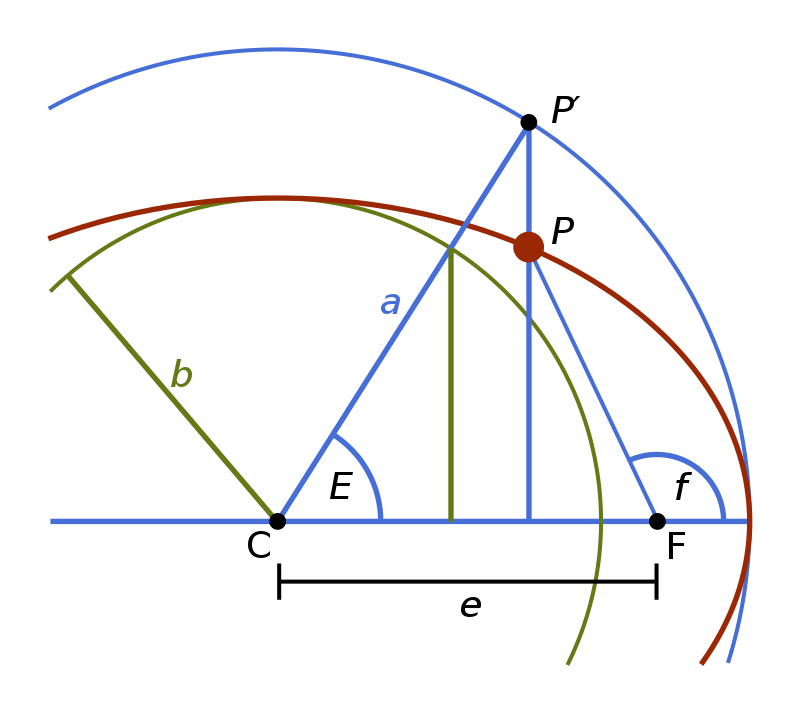
\includegraphics[width=0.4\textwidth]{../images/Eccentric_and_True_Anomaly.png}
	\caption{(Wikipedia, 2020c).} \label{Figure 2.c}
\end{figure}


    \hypertarget{code-showing-variation-in-mean-eccentric-true-anomaly}{%
\subsection{Code Showing Variation in Mean, Eccentric, True Anomaly}\label{code-showing-variation-in-mean-eccentric-true-anomaly}}

Note that the full annotated code can be found in section \ref{the-code}.

    \begin{tcolorbox}[breakable, size=fbox, boxrule=1pt, pad at break*=1mm,colback=cellbackground, colframe=cellborder]
\prompt{In}{incolor}{1}{\boxspacing}
\begin{Verbatim}[commandchars=\\\{\}]
\PY{k+kn}{import} \PY{n+nn}{numpy} \PY{k}{as} \PY{n+nn}{np}
\PY{k+kn}{import} \PY{n+nn}{matplotlib}\PY{n+nn}{.}\PY{n+nn}{pyplot} \PY{k}{as} \PY{n+nn}{plt}
\PY{k+kn}{from} \PY{n+nn}{matplotlib}\PY{n+nn}{.}\PY{n+nn}{pyplot} \PY{k+kn}{import} \PY{n}{figure}


\PY{k}{def} \PY{n+nf}{get\PYZus{}mean\PYZus{}anomaly}\PY{p}{(}\PY{n}{t}\PY{p}{,} \PY{n}{period}\PY{p}{)}\PY{p}{:} 
    \PY{k}{return} \PY{p}{(}\PY{l+m+mi}{2}\PY{o}{*}\PY{n}{np}\PY{o}{.}\PY{n}{pi}\PY{p}{)} \PY{o}{*} \PY{n}{t}\PY{o}{/}\PY{n}{period}           
    
\PY{k}{def} \PY{n+nf}{f}\PY{p}{(}\PY{n}{e}\PY{p}{,} \PY{n}{E}\PY{p}{,} \PY{n}{M}\PY{p}{)}\PY{p}{:}
    \PY{k}{return} \PY{n}{E} \PY{o}{\PYZhy{}} \PY{p}{(}\PY{n}{e} \PY{o}{*} \PY{n}{np}\PY{o}{.}\PY{n}{sin}\PY{p}{(}\PY{n}{E}\PY{p}{)}\PY{p}{)} \PY{o}{\PYZhy{}} \PY{n}{M}

\PY{k}{def} \PY{n+nf}{f\PYZus{}prime}\PY{p}{(}\PY{n}{e}\PY{p}{,} \PY{n}{E}\PY{p}{)}\PY{p}{:}
    \PY{k}{return} \PY{l+m+mi}{1} \PY{o}{\PYZhy{}} \PY{p}{(}\PY{n}{e} \PY{o}{*} \PY{n}{np}\PY{o}{.}\PY{n}{cos}\PY{p}{(}\PY{n}{E}\PY{p}{)}\PY{p}{)}

\PY{k}{def} \PY{n+nf}{get\PYZus{}eccentric\PYZus{}anomaly}\PY{p}{(}\PY{n}{e}\PY{p}{,} \PY{n}{M}\PY{p}{)}\PY{p}{:}        
    \PY{n}{x} \PY{o}{=} \PY{n}{M} \PY{c+c1}{\PYZsh{} the mean anomaly is close to the eccentric anomaly and will converge quicker}
    \PY{n}{x\PYZus{}1} \PY{o}{=} \PY{n}{M} \PY{c+c1}{\PYZsh{} initialise}

    \PY{n}{tolerance} \PY{o}{=} \PY{l+m+mi}{10}\PY{o}{*}\PY{o}{*}\PY{p}{(}\PY{o}{\PYZhy{}}\PY{l+m+mi}{10}\PY{p}{)} \PY{c+c1}{\PYZsh{} 10\PYZhy{}digit accuracy is desired}
    \PY{n}{epsilon} \PY{o}{=} \PY{l+m+mi}{10}\PY{o}{*}\PY{o}{*}\PY{p}{(}\PY{o}{\PYZhy{}}\PY{l+m+mi}{15}\PY{p}{)} \PY{c+c1}{\PYZsh{} minimum divisor }
    \PY{n}{solved} \PY{o}{=} \PY{k+kc}{False}

    \PY{k}{while} \PY{k+kc}{True}\PY{p}{:}                    
        \PY{n}{y} \PY{o}{=} \PY{n}{f}\PY{p}{(}\PY{n}{e}\PY{p}{,} \PY{n}{x}\PY{p}{,} \PY{n}{M}\PY{p}{)}
        \PY{n}{y\PYZus{}prime} \PY{o}{=} \PY{n}{f\PYZus{}prime}\PY{p}{(}\PY{n}{e}\PY{p}{,} \PY{n}{x}\PY{p}{)}
        \PY{c+c1}{\PYZsh{} don\PYZsq{}t want to divide by too small a number }
        \PY{k}{if} \PY{p}{(}\PY{n+nb}{abs}\PY{p}{(}\PY{n}{y\PYZus{}prime}\PY{p}{)} \PY{o}{\PYZgt{}}\PY{o}{=} \PY{n}{epsilon}\PY{p}{)}\PY{p}{:}  
            \PY{n}{x\PYZus{}1} \PY{o}{=} \PY{n}{x} \PY{o}{\PYZhy{}} \PY{n}{y}\PY{o}{/}\PY{p}{(}\PY{n}{y\PYZus{}prime}\PY{p}{)}
            \PY{c+c1}{\PYZsh{} if the result is within the desired tolerance}
            \PY{k}{if} \PY{p}{(}\PY{n+nb}{abs}\PY{p}{(}\PY{n}{x\PYZus{}1} \PY{o}{\PYZhy{}} \PY{n}{x}\PY{p}{)} \PY{o}{\PYZlt{}}\PY{o}{=} \PY{n}{tolerance}\PY{p}{)}\PY{p}{:} 
                \PY{n}{solved} \PY{o}{=} \PY{k+kc}{True}
                \PY{k}{break}
            \PY{k}{else}\PY{p}{:}
                \PY{n}{x} \PY{o}{=} \PY{n}{x\PYZus{}1} \PY{c+c1}{\PYZsh{} update x to restart}
        \PY{k}{else}\PY{p}{:}
            \PY{k}{continue}

    \PY{k}{if} \PY{n}{solved}\PY{p}{:}
        \PY{k}{return} \PY{n}{x\PYZus{}1}
    \PY{k}{else}\PY{p}{:}
        \PY{k}{raise} \PY{n+ne}{ValueError}\PY{p}{(}\PY{l+s+s2}{\PYZdq{}}\PY{l+s+s2}{no convergence}\PY{l+s+s2}{\PYZdq{}}\PY{p}{)}

\PY{k}{def} \PY{n+nf}{get\PYZus{}true\PYZus{}anomaly}\PY{p}{(}\PY{n}{e}\PY{p}{,} \PY{n}{E}\PY{p}{)}\PY{p}{:}
        \PY{n}{cosE} \PY{o}{=} \PY{n}{np}\PY{o}{.}\PY{n}{cos}\PY{p}{(}\PY{n}{E}\PY{p}{)}
        \PY{n}{diff} \PY{o}{=} \PY{n}{cosE} \PY{o}{\PYZhy{}} \PY{n}{e}
        \PY{n}{cosNu} \PY{o}{=} \PY{n}{diff}\PY{o}{/}\PY{p}{(}\PY{l+m+mi}{1} \PY{o}{\PYZhy{}} \PY{n}{e} \PY{o}{*} \PY{n}{cosE}\PY{p}{)}
        \PY{n}{nu} \PY{o}{=} \PY{n}{np}\PY{o}{.}\PY{n}{arccos}\PY{p}{(}\PY{n}{cosNu}\PY{p}{)}
        \PY{k}{return} \PY{n}{nu}
           
\PY{k}{def} \PY{n+nf}{main}\PY{p}{(}\PY{p}{)}\PY{p}{:}
    \PY{l+s+sd}{\PYZdq{}\PYZdq{}\PYZdq{}}
\PY{l+s+sd}{    Function that graphs the variation in M, E and nu }
\PY{l+s+sd}{    as the planets orbits the star.}
\PY{l+s+sd}{    }
\PY{l+s+sd}{    e: eccentricity of the orbit }
\PY{l+s+sd}{    period: period of the orbit in days}
\PY{l+s+sd}{    \PYZdq{}\PYZdq{}\PYZdq{}}
    \PY{n}{sample\PYZus{}parameters} \PY{o}{=} \PY{p}{\PYZob{}}\PY{l+s+s2}{\PYZdq{}}\PY{l+s+s2}{e}\PY{l+s+s2}{\PYZdq{}}\PY{p}{:}\PY{l+m+mf}{0.5}\PY{p}{,} \PY{l+s+s2}{\PYZdq{}}\PY{l+s+s2}{period}\PY{l+s+s2}{\PYZdq{}}\PY{p}{:} \PY{l+m+mi}{24}\PY{p}{\PYZcb{}}
    \PY{n}{step} \PY{o}{=} \PY{l+m+mi}{3600}
    \PY{n}{timestamps} \PY{o}{=} \PY{n}{np}\PY{o}{.}\PY{n}{linspace}\PY{p}{(}\PY{l+m+mi}{0}\PY{p}{,} \PY{n}{sample\PYZus{}parameters}\PY{p}{[}\PY{l+s+s2}{\PYZdq{}}\PY{l+s+s2}{period}\PY{l+s+s2}{\PYZdq{}}\PY{p}{]}\PY{p}{,} \PY{n}{step}\PY{p}{)}
    
    \PY{n}{M\PYZus{}list} \PY{o}{=} \PY{p}{[}\PY{p}{]}\PY{p}{;} \PY{n}{E\PYZus{}list} \PY{o}{=} \PY{p}{[}\PY{p}{]}\PY{p}{;} \PY{n}{nu\PYZus{}list} \PY{o}{=} \PY{p}{[}\PY{p}{]} \PY{c+c1}{\PYZsh{} initialise arrays }
    
    \PY{k}{for} \PY{n}{time} \PY{o+ow}{in} \PY{n}{timestamps}\PY{p}{:}
        \PY{n}{M} \PY{o}{=} \PY{n}{get\PYZus{}mean\PYZus{}anomaly}\PY{p}{(}\PY{n}{time}\PY{p}{,} \PY{n}{sample\PYZus{}parameters}\PY{p}{[}\PY{l+s+s2}{\PYZdq{}}\PY{l+s+s2}{period}\PY{l+s+s2}{\PYZdq{}}\PY{p}{]}\PY{p}{)}           
        \PY{n}{E} \PY{o}{=} \PY{n}{get\PYZus{}eccentric\PYZus{}anomaly}\PY{p}{(}\PY{n}{sample\PYZus{}parameters}\PY{p}{[}\PY{l+s+s2}{\PYZdq{}}\PY{l+s+s2}{e}\PY{l+s+s2}{\PYZdq{}}\PY{p}{]}\PY{p}{,} \PY{n}{M}\PY{p}{)}
        \PY{n}{nu} \PY{o}{=} \PY{n}{get\PYZus{}true\PYZus{}anomaly}\PY{p}{(}\PY{n}{sample\PYZus{}parameters}\PY{p}{[}\PY{l+s+s2}{\PYZdq{}}\PY{l+s+s2}{e}\PY{l+s+s2}{\PYZdq{}}\PY{p}{]}\PY{p}{,} \PY{n}{E}\PY{p}{)}
        \PY{k}{if} \PY{n}{E} \PY{o}{\PYZgt{}}\PY{o}{=} \PY{n}{np}\PY{o}{.}\PY{n}{pi}\PY{p}{:}
            \PY{n}{nu} \PY{o}{=} \PY{p}{(}\PY{l+m+mi}{2}\PY{o}{*}\PY{n}{np}\PY{o}{.}\PY{n}{pi}\PY{p}{)} \PY{o}{\PYZhy{}}\PY{n}{nu}
        \PY{n}{M\PYZus{}list}\PY{o}{.}\PY{n}{append}\PY{p}{(}\PY{n}{M}\PY{p}{)}\PY{p}{;} \PY{n}{E\PYZus{}list}\PY{o}{.}\PY{n}{append}\PY{p}{(}\PY{n}{E}\PY{p}{)}\PY{p}{;} \PY{n}{nu\PYZus{}list}\PY{o}{.}\PY{n}{append}\PY{p}{(}\PY{n}{nu}\PY{p}{)}
        
    \PY{n}{figure}\PY{p}{(}\PY{n}{num}\PY{o}{=}\PY{l+m+mi}{3}\PY{p}{,} \PY{n}{figsize}\PY{o}{=}\PY{p}{(}\PY{l+m+mi}{10}\PY{p}{,} \PY{l+m+mi}{8}\PY{p}{)}\PY{p}{,} \PY{n}{dpi}\PY{o}{=}\PY{l+m+mi}{80}\PY{p}{,} \PY{n}{facecolor}\PY{o}{=}\PY{l+s+s2}{\PYZdq{}}\PY{l+s+s2}{w}\PY{l+s+s2}{\PYZdq{}}\PY{p}{,} \PY{n}{edgecolor}\PY{o}{=}\PY{l+s+s2}{\PYZdq{}}\PY{l+s+s2}{b}\PY{l+s+s2}{\PYZdq{}}\PY{p}{)}
    
    \PY{n}{plt}\PY{o}{.}\PY{n}{plot}\PY{p}{(}\PY{n}{timestamps}\PY{p}{,} \PY{n}{M\PYZus{}list}\PY{p}{,} \PY{l+s+s2}{\PYZdq{}}\PY{l+s+s2}{r\PYZhy{}}\PY{l+s+s2}{\PYZdq{}}\PY{p}{,} \PY{n}{label}\PY{o}{=}\PY{l+s+s2}{\PYZdq{}}\PY{l+s+s2}{Mean Anomaly}\PY{l+s+s2}{\PYZdq{}}\PY{p}{)}
    \PY{n}{plt}\PY{o}{.}\PY{n}{plot}\PY{p}{(}\PY{n}{timestamps}\PY{p}{,} \PY{n}{E\PYZus{}list}\PY{p}{,} \PY{l+s+s2}{\PYZdq{}}\PY{l+s+s2}{b\PYZhy{}}\PY{l+s+s2}{\PYZdq{}}\PY{p}{,} \PY{n}{label}\PY{o}{=}\PY{l+s+s2}{\PYZdq{}}\PY{l+s+s2}{Eccentric Anomaly}\PY{l+s+s2}{\PYZdq{}}\PY{p}{)}
    \PY{n}{plt}\PY{o}{.}\PY{n}{plot}\PY{p}{(}\PY{n}{timestamps}\PY{p}{,} \PY{n}{nu\PYZus{}list}\PY{p}{,} \PY{l+s+s2}{\PYZdq{}}\PY{l+s+s2}{g\PYZhy{}}\PY{l+s+s2}{\PYZdq{}}\PY{p}{,} \PY{n}{label}\PY{o}{=}\PY{l+s+s2}{\PYZdq{}}\PY{l+s+s2}{True Anomaly}\PY{l+s+s2}{\PYZdq{}}\PY{p}{)}
    \PY{n}{plt}\PY{o}{.}\PY{n}{title}\PY{p}{(}\PY{l+s+s2}{\PYZdq{}}\PY{l+s+s2}{Variation of M, E and nu for a Given Orbit}\PY{l+s+s2}{\PYZdq{}}\PY{p}{)}
    
    \PY{n}{plt}\PY{o}{.}\PY{n}{xlabel}\PY{p}{(}\PY{l+s+s2}{\PYZdq{}}\PY{l+s+s2}{Period/days}\PY{l+s+s2}{\PYZdq{}}\PY{p}{)}
    \PY{n}{plt}\PY{o}{.}\PY{n}{ylabel}\PY{p}{(}\PY{l+s+s2}{\PYZdq{}}\PY{l+s+s2}{Angle/radians}\PY{l+s+s2}{\PYZdq{}}\PY{p}{)}
    \PY{n}{plt}\PY{o}{.}\PY{n}{yticks}\PY{p}{(}\PY{p}{[}\PY{n}{np}\PY{o}{.}\PY{n}{pi}\PY{o}{/}\PY{l+m+mi}{2}\PY{p}{,} \PY{n}{np}\PY{o}{.}\PY{n}{pi}\PY{p}{,} \PY{l+m+mi}{3}\PY{o}{*}\PY{n}{np}\PY{o}{.}\PY{n}{pi}\PY{o}{/}\PY{l+m+mi}{2}\PY{p}{,} \PY{l+m+mi}{2}\PY{o}{*}\PY{n}{np}\PY{o}{.}\PY{n}{pi}\PY{p}{]}\PY{p}{)}

    \PY{n}{plt}\PY{o}{.}\PY{n}{legend}\PY{p}{(}\PY{p}{)}
    \PY{n}{plt}\PY{o}{.}\PY{n}{grid}\PY{p}{(}\PY{k+kc}{True}\PY{p}{)}
   
    \PY{n}{plt}\PY{o}{.}\PY{n}{show}\PY{p}{(}\PY{p}{)}

\PY{n}{main}\PY{p}{(}\PY{p}{)}
\end{Verbatim}
\end{tcolorbox}

\begin{figure}[hbt!]
	\figuretitle{Output:}
	\centering	
   	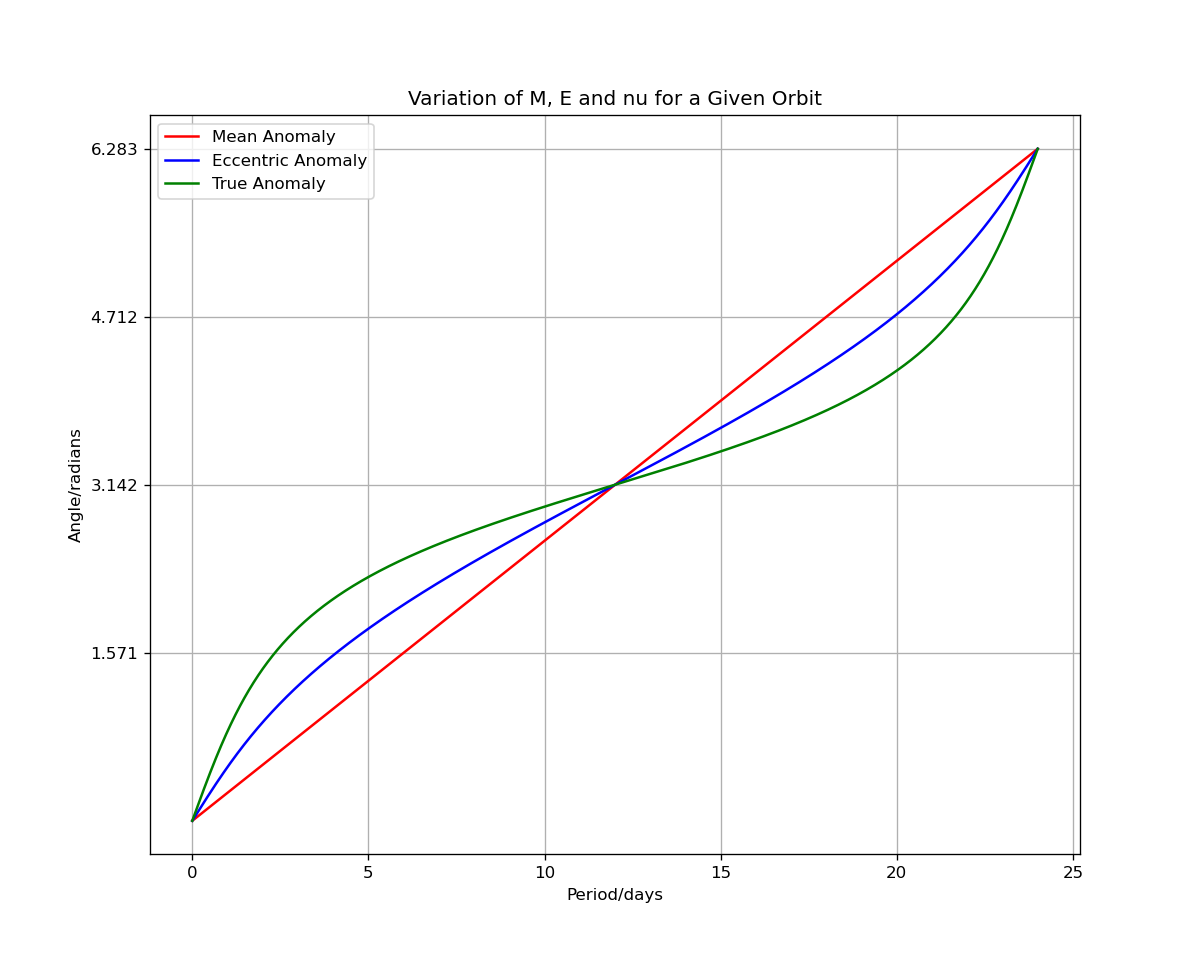
\includegraphics[width=0.8\textwidth]{../matplotlib_graphs/anomalies.png}
\end{figure}
    
    
    \hypertarget{the-light-curve}{%
\subsection{The Light Curve}\label{the-light-curve}}

Predicting the light curve relies on understanding several stellar
parameters, the most important of these being the formulae giving a
``fast and accurate means of computing light curves using limb-darkening
coefficients'' (Mandel and Agol, 2002). In order to produce the
normalised light curve, we need to calculate the ratio between the
unobstructed and obstructed blocked flux. The parameters of the transit
curve are given in the diagram below.

The \emph{total} duration of the transit is
\(T_{tot} = t_{IV} - t_{I}\); the \emph{full} duration is
\(T_{full} = t_{III} - t_{II}\), the \emph{ingress} duration is
\(\tau_{ing} = t_{II} - t_{I}\); the \emph{egress} duration is
\(\tau_{egr} = t_{IV} - t_{III}\). (Winn, 2010)


\begin{figure}[!ht]
	\centering
	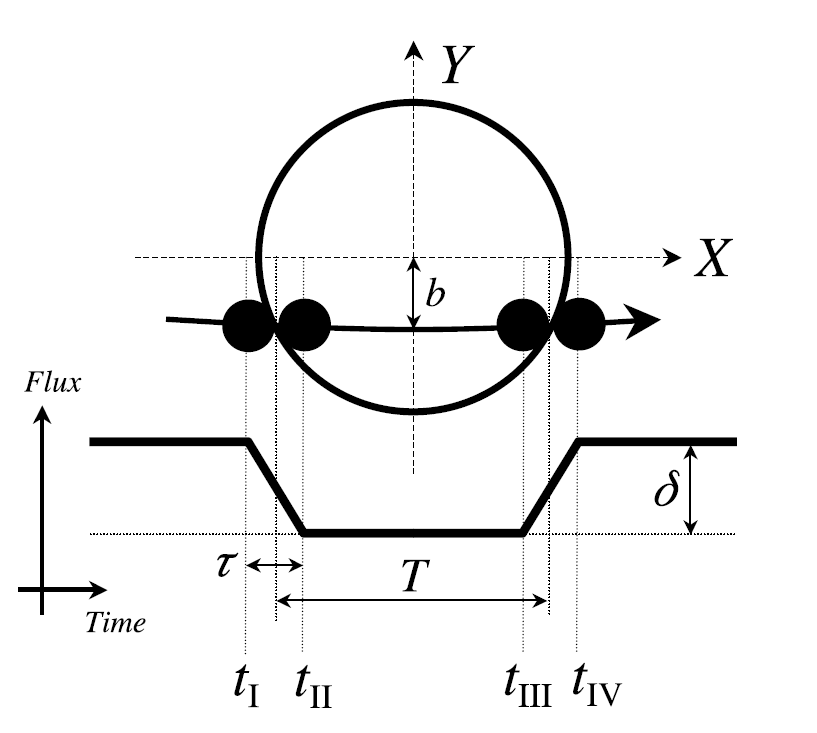
\includegraphics[width=0.4\textwidth]{../images/transit_flux.png}
	\caption{Figure showing the main parameters of the transit of the planet (Winn, 2010).} \label{Figure 2.d}
\end{figure}



    \hypertarget{flux}{%
\subsubsection{Flux}\label{flux}}

Mandel and Agol (2002) give the equations that describe the normalised
observed flux, calculated based on \(d\) the centre-to-centre distance
between the star and the planet, which is in turn affected by the
eccentric anomaly, \(E\). This relationship is described as follows:

\begin{equation*}
d = a\cos{E}
\end{equation*}

The below gives the function for a uniform light source:

\begin{figure}[H]
	\centering
	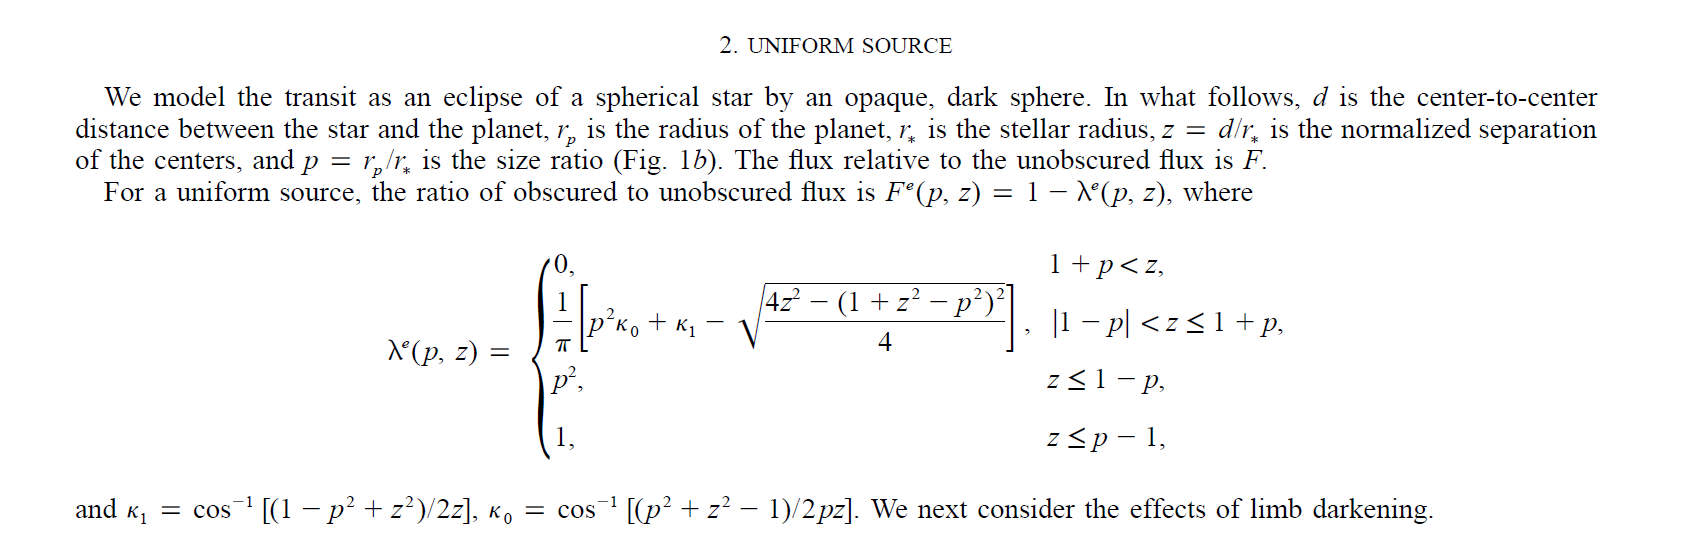
\includegraphics[width=\textwidth]{../images/uniform_source.png}
	\label{Figure 2.e}
\end{figure}

    \hypertarget{limb-darkening}{%
\subsubsection{Limb Darkening}\label{limb-darkening}}

This is a mathematical model that accounts for the fact that stars are significantly dimmer at the edges; using limb darkening equations, we can integrate this function for the entire surface of the star.

The intensity of the stellar output has been described by Mandel and Agol (2002).

\hypertarget{quadratic-limb-darkening}{%
\subsubsection{Quadratic Limb Darkening}\label{quadratic-limb-darkening}}

This is the main model that we will use in this project to increase
computational efficiency.

\begin{equation*}
I(r) = 1 - \gamma_{1}(1 - \mu) - \gamma_{2}(1 - \mu)^{2}
\end{equation*}

where \(\mu = \sqrt{(1 - r^{2})}\) (\(r\) is the normalised radial
coordinate) and \(0 \leqslant \mu \leqslant 1\) and \(\gamma\) is a free
parameter constant describing the limb darkening profile
(\(\gamma_{1} + \gamma_{2} < 1\)).

\hypertarget{non-linear-limb-darkening}{%
\subsubsection{Non-linear Limb Darkening}\label{non-linear-limb-darkening}}

\begin{equation*}
I(\mu) = 1 - \sum_{n = 1}^{4} c_{n}(1 - \mu^{\frac{n}{2}})
\end{equation*}

    \hypertarget{code-showing-the-quadratic-limb-darkening-profile}{%
\subsubsection{Code Showing the Quadratic Limb Darkening Profile}\label{code-showing-the-quadratic-limb-darkening-profile}}

    \begin{tcolorbox}[breakable, size=fbox, boxrule=1pt, pad at break*=1mm,colback=cellbackground, colframe=cellborder]
\prompt{In}{incolor}{2}{\boxspacing}
\begin{Verbatim}[commandchars=\\\{\}]
\PY{k+kn}{import} \PY{n+nn}{numpy} \PY{k}{as} \PY{n+nn}{np}
\PY{k+kn}{import} \PY{n+nn}{matplotlib}\PY{n+nn}{.}\PY{n+nn}{pyplot} \PY{k}{as} \PY{n+nn}{plt}
\PY{k+kn}{from} \PY{n+nn}{matplotlib}\PY{n+nn}{.}\PY{n+nn}{pyplot} \PY{k+kn}{import} \PY{n}{figure}

\PY{n}{gamma} \PY{o}{=} \PY{p}{(}\PY{l+m+mf}{0.5}\PY{p}{,} \PY{l+m+mf}{0.1}\PY{p}{)} \PY{c+c1}{\PYZsh{} free parameter constants describing the limb darkening profile}

\PY{k}{def} \PY{n+nf}{intensity}\PY{p}{(}\PY{n}{r}\PY{p}{)}\PY{p}{:}
    \PY{n}{mu} \PY{o}{=} \PY{p}{(}\PY{l+m+mi}{1} \PY{o}{\PYZhy{}} \PY{n}{r}\PY{o}{*}\PY{o}{*}\PY{l+m+mi}{2}\PY{p}{)} \PY{o}{*}\PY{o}{*} \PY{l+m+mf}{0.5}
    \PY{n}{k} \PY{o}{=} \PY{l+m+mi}{1} \PY{o}{\PYZhy{}} \PY{n}{mu}
    \PY{k}{return} \PY{l+m+mi}{1} \PY{o}{\PYZhy{}} \PY{n}{gamma}\PY{p}{[}\PY{l+m+mi}{0}\PY{p}{]}\PY{o}{*}\PY{n}{k} \PY{o}{\PYZhy{}} \PY{n}{gamma}\PY{p}{[}\PY{l+m+mi}{1}\PY{p}{]}\PY{o}{*}\PY{p}{(}\PY{n}{k}\PY{o}{*}\PY{o}{*}\PY{l+m+mi}{2}\PY{p}{)}

\PY{n}{figure}\PY{p}{(}\PY{n}{num}\PY{o}{=}\PY{l+m+mi}{3}\PY{p}{,} \PY{n}{figsize}\PY{o}{=}\PY{p}{(}\PY{l+m+mi}{6}\PY{p}{,} \PY{l+m+mi}{4}\PY{p}{)}\PY{p}{,} \PY{n}{dpi}\PY{o}{=}\PY{l+m+mi}{80}\PY{p}{,} \PY{n}{facecolor}\PY{o}{=}\PY{l+s+s2}{\PYZdq{}}\PY{l+s+s2}{w}\PY{l+s+s2}{\PYZdq{}}\PY{p}{,} \PY{n}{edgecolor}\PY{o}{=}\PY{l+s+s2}{\PYZdq{}}\PY{l+s+s2}{b}\PY{l+s+s2}{\PYZdq{}}\PY{p}{)}

\PY{n}{x} \PY{o}{=} \PY{n}{np}\PY{o}{.}\PY{n}{linspace}\PY{p}{(}\PY{l+m+mi}{0}\PY{p}{,} \PY{l+m+mi}{1}\PY{p}{,} \PY{l+m+mi}{3600}\PY{p}{)}
\PY{n}{y} \PY{o}{=} \PY{n+nb}{list}\PY{p}{(}\PY{n+nb}{map}\PY{p}{(}\PY{n}{intensity}\PY{p}{,} \PY{n}{x}\PY{p}{)}\PY{p}{)}

\PY{n}{plt}\PY{o}{.}\PY{n}{plot}\PY{p}{(}\PY{n}{x}\PY{p}{,}\PY{n}{y}\PY{p}{,} \PY{n}{color}\PY{o}{=}\PY{l+s+s2}{\PYZdq{}}\PY{l+s+s2}{b}\PY{l+s+s2}{\PYZdq{}}\PY{p}{)}
\PY{n}{plt}\PY{o}{.}\PY{n}{title}\PY{p}{(}\PY{l+s+s2}{\PYZdq{}}\PY{l+s+s2}{Quadratic Limb Darkening Curve}\PY{l+s+s2}{\PYZdq{}}\PY{p}{)}
\PY{n}{plt}\PY{o}{.}\PY{n}{xlabel}\PY{p}{(}\PY{l+s+s2}{\PYZdq{}}\PY{l+s+s2}{Normalised Distance from Centre of Star}\PY{l+s+s2}{\PYZdq{}}\PY{p}{)}
\PY{n}{plt}\PY{o}{.}\PY{n}{ylabel}\PY{p}{(}\PY{l+s+s2}{\PYZdq{}}\PY{l+s+s2}{Normalised Flux}\PY{l+s+s2}{\PYZdq{}}\PY{p}{)}
\PY{n}{plt}\PY{o}{.}\PY{n}{grid}\PY{p}{(}\PY{k+kc}{True}\PY{p}{)}
\PY{n}{plt}\PY{o}{.}\PY{n}{show}\PY{p}{(}\PY{p}{)}
\end{Verbatim}
\end{tcolorbox}

\begin{figure}[H]
	\figuretitle{Output:}
	\centering
	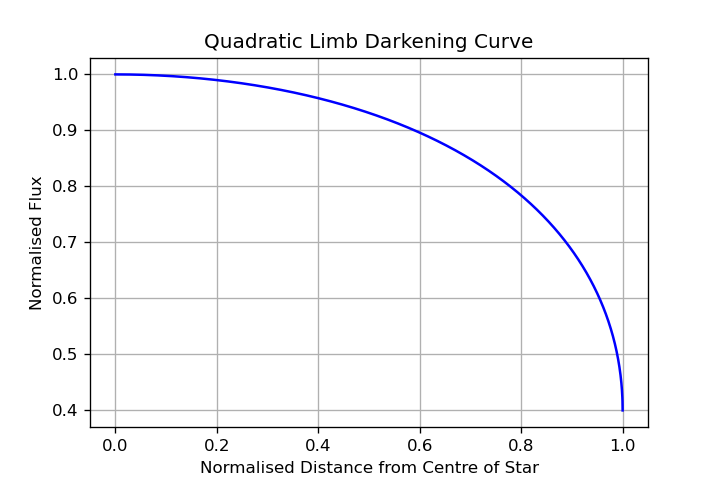
\includegraphics[width=0.75\textwidth]{../matplotlib_graphs/limb_darkening.png}
\end{figure}    
    
This seems reasonable. See the fully annotated code in Section 3.

    \hypertarget{full-transit-curve}{%
\subsubsection{Full Transit Curve}\label{full-transit-curve}}

These equations are combined with the below to give the full transit
curve:

\begin{figure}[!ht]
	\centering
	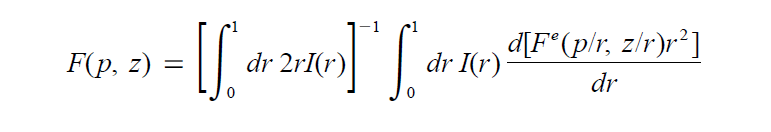
\includegraphics[width=0.5\textwidth]{../images/flux_eq.png}
	\label{Figure 2.f}
\end{figure}

    \hypertarget{radial-velocity}{%
\subsection{Radial Velocity}\label{radial-velocity}}

Predicting the radial velocity also requires an accurate model of the
motion of both the exoplanet and parent star; once the mass of both are given, and the motion of the planet can be modelled, the motion of the star can be found. The formulae used in this project relating true anomaly, \(\nu\), and variations in radial velocity are derived \href{http://exoplanets.astro.yale.edu/workshop/EPRV/Bibliography_files/Radial_Velocity.pdf}{here} in \emph{Radial Velocity} (Lovis, 2011).

Whilst the model includes the calculation of the change in wavelength
due to the Doppler effect, below in section 4 we will focus on the
measurement produced for radial velocity, as this is the main focus of
most academic literature (Doppler spectroscopy being the raw data
measured from telescopes). It is stressed that relativistic Doppler is
\emph{not} used in this project as the increase in precision is
negligible given the range of uncertainty in the initial readings.

\hypertarget{radial-velocity-equation}{%
\subsubsection{Radial Velocity Equation}\label{radial-velocity-equation}}

The equation for radial velocity used in this model is given by Lovis
and Fischer (2010).

\begin{figure}[H]
	\centering
	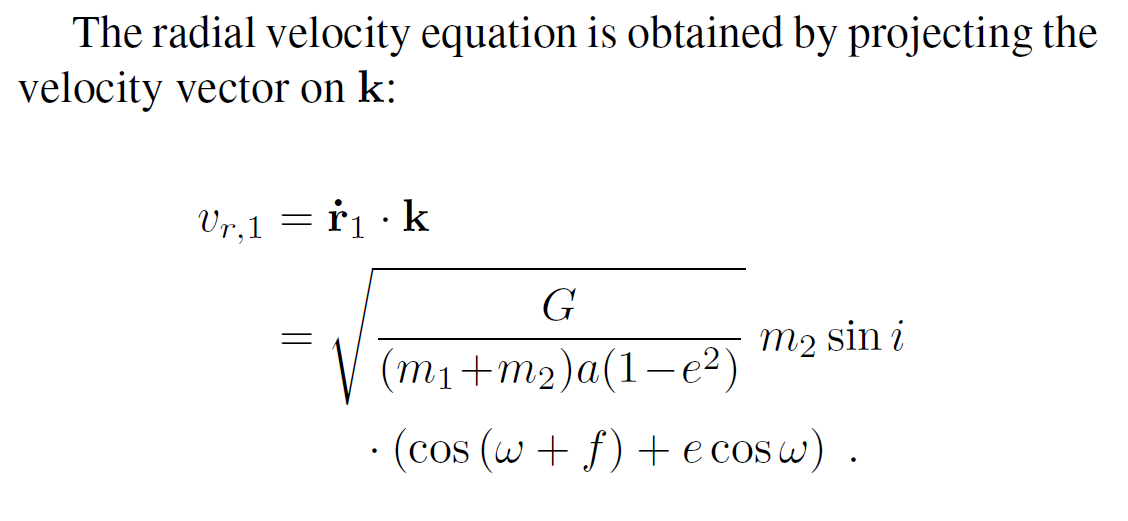
\includegraphics[width=0.5\textwidth]{../images/radial_velocity.png}
	\label{Figure 2.g}
\end{figure}

From there we can derive the semi-amplitude of the radial velocity: \(K\).

\begin{figure}[H]
   	\centering
   	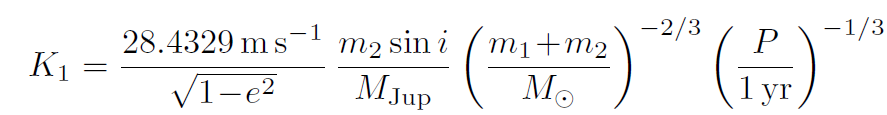
\includegraphics[width=0.5\textwidth]{../images/K_star.png}
   	\label{Figure 2.h}
\end{figure}

    \hypertarget{an-interlude-on-units}{%
\subsection{An Interlude on Units}\label{an-interlude-on-units}}

In this model, the following units are used: 

\begin{itemize}
	\item Length: Astronomical Units (AU)
	\item Mass: Solar Mass
	\item Time: Days
	\item Angle: Radians
\end{itemize}

Hence, whilst some values such as \(i\) (inclination) are inputted into
the code in other units (e.g. degrees), these are converted in the code.

\begin{center}\rule{0.5\linewidth}{0.5pt}\end{center}
    \hypertarget{the-exoplanet-model}{%
\section{The Exoplanet Model}\label{the-exoplanet-model}}

\hypertarget{notes-on-the-code}{%
\subsection{Notes on the Code}\label{notes-on-the-code}}

In this code, we set up constants with global scope. Then, both a Planet
and Star class are initialised, which are then passed into the
BinarySystem class. BinarySystem includes two the main methods that can
be used to output graphical results: \emph{.transit}, which produces a
light curve graph of the transit, and \emph{.radial\_velocity}, which
produces a graph of radial velocity variations. Other methods and
attributes are included, but these are not designed to be ran
individually as they are not stand-alone functions.

\hypertarget{the-code}{%
\subsection{The Code}\label{the-code}}

    \begin{tcolorbox}[breakable, size=fbox, boxrule=1pt, pad at break*=1mm,colback=cellbackground, colframe=cellborder]
\prompt{In}{incolor}{3}{\boxspacing}
\begin{Verbatim}[commandchars=\\\{\}]
\PY{c+c1}{\PYZsh{} Set\PYZhy{}up of dependencies needed for code }

\PY{k+kn}{from} \PY{n+nn}{\PYZus{}\PYZus{}future\PYZus{}\PYZus{}} \PY{k+kn}{import} \PY{n}{division}
\PY{k+kn}{import} \PY{n+nn}{numpy} \PY{k}{as} \PY{n+nn}{np}
\PY{k+kn}{from} \PY{n+nn}{numpy}\PY{n+nn}{.}\PY{n+nn}{random} \PY{k+kn}{import} \PY{n}{rand}

\PY{c+c1}{\PYZsh{} defining of constants }
\PY{n}{pi} \PY{o}{=} \PY{n}{np}\PY{o}{.}\PY{n}{pi}
\PY{n}{N\PYZus{}stepsize} \PY{o}{=} \PY{l+m+mi}{3600} \PY{c+c1}{\PYZsh{} general step size for computations (integration and differention from 0 to 1)}
\PY{n}{SMALL\PYZus{}NUM} \PY{o}{=} \PY{l+m+mf}{0.1}\PY{o}{/}\PY{n}{N\PYZus{}stepsize}
\PY{n}{gamma} \PY{o}{=} \PY{p}{(}\PY{l+m+mf}{0.5}\PY{p}{,} \PY{l+m+mf}{0.1}\PY{p}{)} \PY{c+c1}{\PYZsh{} free parameter constants describing the limb darkening profile}
\PY{n}{V\PYZus{}0} \PY{o}{=} \PY{l+m+mi}{0} \PY{c+c1}{\PYZsh{} mean radial velocity of the star\PYZhy{}planet centre of mass}

\PY{n}{g\PYZus{}constant\PYZus{}SI} \PY{o}{=} \PY{l+m+mf}{6.6743}\PY{o}{*}\PY{p}{(}\PY{l+m+mi}{10}\PY{o}{*}\PY{o}{*}\PY{o}{\PYZhy{}}\PY{l+m+mi}{11}\PY{p}{)} \PY{c+c1}{\PYZsh{} here g is defined in m**3 * kg**\PYZhy{}1 * s**\PYZhy{}2}
\PY{n}{k} \PY{o}{=} \PY{p}{(}\PY{l+m+mf}{1.495978707} \PY{o}{*} \PY{p}{(}\PY{l+m+mi}{10}\PY{o}{*}\PY{o}{*}\PY{l+m+mi}{11}\PY{p}{)}\PY{p}{)}\PY{o}{*}\PY{o}{*}\PY{l+m+mi}{3} \PY{o}{/} \PY{p}{(}\PY{l+m+mf}{1.988478}\PY{o}{*}\PY{p}{(}\PY{l+m+mi}{10}\PY{o}{*}\PY{o}{*}\PY{l+m+mi}{30}\PY{p}{)} \PY{o}{*} \PY{p}{(}\PY{l+m+mi}{24} \PY{o}{*} \PY{l+m+mi}{60} \PY{o}{*} \PY{l+m+mi}{60}\PY{p}{)}\PY{o}{*}\PY{o}{*}\PY{l+m+mi}{2}\PY{p}{)} \PY{c+c1}{\PYZsh{} k is a dimensionless conversion factor}
\PY{n}{g\PYZus{}constant} \PY{o}{=} \PY{n}{g\PYZus{}constant\PYZus{}SI}\PY{o}{/}\PY{n}{k} \PY{c+c1}{\PYZsh{} here g is defined in AU**3 * solar\PYZus{}mass**\PYZhy{}1 * days**\PYZhy{}2}

\PY{n}{c\PYZus{}constant\PYZus{}SI} \PY{o}{=} \PY{l+m+mi}{299792458} \PY{c+c1}{\PYZsh{} here c is defined in m/s}
\PY{n}{kappa} \PY{o}{=} \PY{p}{(}\PY{l+m+mi}{24} \PY{o}{*} \PY{l+m+mi}{60} \PY{o}{*} \PY{l+m+mi}{60}\PY{p}{)}\PY{o}{/} \PY{p}{(}\PY{l+m+mf}{1.495978707} \PY{o}{*} \PY{p}{(}\PY{l+m+mi}{10}\PY{o}{*}\PY{o}{*}\PY{l+m+mi}{11}\PY{p}{)}\PY{p}{)} \PY{c+c1}{\PYZsh{} kappa is a dimensionless conversion factor}
\PY{n}{c\PYZus{}constant} \PY{o}{=} \PY{n}{c\PYZus{}constant\PYZus{}SI}\PY{o}{/}\PY{n}{kappa} \PY{c+c1}{\PYZsh{} here c is defined in AU/day}


\PY{n}{DEBUG} \PY{o}{=} \PY{k+kc}{False}


\PY{l+s+sd}{\PYZdq{}\PYZdq{}\PYZdq{}}
\PY{l+s+sd}{The dictionary \PYZsq{}convert\PYZsq{} below converts from the units}
\PY{l+s+sd}{specified in the keys to the units below}

\PY{l+s+sd}{length \PYZhy{}\PYZgt{} AU}
\PY{l+s+sd}{mass \PYZhy{}\PYZgt{} solar\PYZus{}mass}
\PY{l+s+sd}{time \PYZhy{}\PYZgt{} days}
\PY{l+s+sd}{angle \PYZhy{}\PYZgt{} radians}
\PY{l+s+sd}{\PYZdq{}\PYZdq{}\PYZdq{}}

\PY{c+c1}{\PYZsh{} ratio of 1:units}

\PY{n}{convert} \PY{o}{=} \PY{p}{\PYZob{}}
    \PY{l+s+s2}{\PYZdq{}}\PY{l+s+s2}{solar\PYZus{}radius}\PY{l+s+s2}{\PYZdq{}}\PY{p}{:} \PY{l+m+mf}{0.00465047}\PY{p}{,}
    \PY{l+s+s2}{\PYZdq{}}\PY{l+s+s2}{solar\PYZus{}mass}\PY{l+s+s2}{\PYZdq{}}\PY{p}{:} \PY{l+m+mi}{1}\PY{p}{,}
    \PY{l+s+s2}{\PYZdq{}}\PY{l+s+s2}{jovian\PYZus{}radius}\PY{l+s+s2}{\PYZdq{}}\PY{p}{:} \PY{l+m+mf}{0.000477895}\PY{p}{,} 
    \PY{l+s+s2}{\PYZdq{}}\PY{l+s+s2}{jovian\PYZus{}mass}\PY{l+s+s2}{\PYZdq{}}\PY{p}{:} \PY{l+m+mf}{0.0009547919}\PY{p}{,} 
    \PY{l+s+s2}{\PYZdq{}}\PY{l+s+s2}{AU}\PY{l+s+s2}{\PYZdq{}}\PY{p}{:} \PY{l+m+mi}{1}\PY{p}{,} 
    \PY{l+s+s2}{\PYZdq{}}\PY{l+s+s2}{years}\PY{l+s+s2}{\PYZdq{}}\PY{p}{:} \PY{l+m+mf}{365.25}\PY{p}{,} 
    \PY{l+s+s2}{\PYZdq{}}\PY{l+s+s2}{degrees}\PY{l+s+s2}{\PYZdq{}}\PY{p}{:} \PY{l+m+mi}{180}\PY{o}{/}\PY{n}{pi}\PY{p}{,} 
    \PY{l+s+s2}{\PYZdq{}}\PY{l+s+s2}{n/a}\PY{l+s+s2}{\PYZdq{}}\PY{p}{:} \PY{l+m+mi}{1}
\PY{p}{\PYZcb{}}
\end{Verbatim}
\end{tcolorbox}

    \begin{tcolorbox}[breakable, size=fbox, boxrule=1pt, pad at break*=1mm,colback=cellbackground, colframe=cellborder]
\prompt{In}{incolor}{4}{\boxspacing}
\begin{Verbatim}[commandchars=\\\{\}]
\PY{c+c1}{\PYZsh{} Set\PYZhy{}up of Star and Planet classes}

\PY{k}{class} \PY{n+nc}{Star}\PY{p}{:}
    \PY{l+s+sd}{\PYZdq{}\PYZdq{}\PYZdq{}}
\PY{l+s+sd}{    Star Object}
\PY{l+s+sd}{    \PYZdq{}\PYZdq{}\PYZdq{}}
    \PY{k}{def} \PY{n+nf+fm}{\PYZus{}\PYZus{}init\PYZus{}\PYZus{}}\PY{p}{(}\PY{n+nb+bp}{self}\PY{p}{,} \PY{n}{mass}\PY{p}{,} \PY{n}{radius}\PY{p}{,} \PY{n}{earth\PYZus{}distance}\PY{o}{=}\PY{l+m+mi}{1}\PY{p}{)}\PY{p}{:}
        \PY{l+s+sd}{\PYZdq{}\PYZdq{}\PYZdq{}}
\PY{l+s+sd}{        Args:}
\PY{l+s+sd}{            mass: solar\PYZus{}mass}
\PY{l+s+sd}{            radius: solar\PYZus{}radius}
\PY{l+s+sd}{            earth\PYZus{}distance: distance from the earth in light years}
\PY{l+s+sd}{            spectral\PYZus{}line: average wavelength of the spectral line.}
\PY{l+s+sd}{        Initialises:}
\PY{l+s+sd}{            raw\PYZus{}mass: solar\PYZus{}mass}
\PY{l+s+sd}{            raw\PYZus{}radius: solar\PYZus{}radius}
\PY{l+s+sd}{            mass: solar\PYZus{}mass}
\PY{l+s+sd}{            radius: AU}
\PY{l+s+sd}{        \PYZdq{}\PYZdq{}\PYZdq{}}
        \PY{n+nb+bp}{self}\PY{o}{.}\PY{n}{raw\PYZus{}mass} \PY{o}{=} \PY{n}{mass}
        \PY{n+nb+bp}{self}\PY{o}{.}\PY{n}{raw\PYZus{}radius} \PY{o}{=} \PY{n}{radius}
        \PY{n+nb+bp}{self}\PY{o}{.}\PY{n}{mass} \PY{o}{=} \PY{n}{mass} \PY{o}{*} \PY{n}{convert}\PY{p}{[}\PY{l+s+s2}{\PYZdq{}}\PY{l+s+s2}{solar\PYZus{}mass}\PY{l+s+s2}{\PYZdq{}}\PY{p}{]}
        \PY{n+nb+bp}{self}\PY{o}{.}\PY{n}{radius} \PY{o}{=} \PY{n}{radius} \PY{o}{*} \PY{n}{convert}\PY{p}{[}\PY{l+s+s2}{\PYZdq{}}\PY{l+s+s2}{solar\PYZus{}radius}\PY{l+s+s2}{\PYZdq{}}\PY{p}{]}
        \PY{n+nb+bp}{self}\PY{o}{.}\PY{n}{earth\PYZus{}distance} \PY{o}{=} \PY{n}{earth\PYZus{}distance}
        \PY{n+nb+bp}{self}\PY{o}{.}\PY{n}{spectral\PYZus{}line} \PY{o}{=} \PY{l+m+mi}{1}
        
\PY{k}{class} \PY{n+nc}{Planet}\PY{p}{:}
    \PY{l+s+sd}{\PYZdq{}\PYZdq{}\PYZdq{}}
\PY{l+s+sd}{    Planet Object}
\PY{l+s+sd}{    \PYZdq{}\PYZdq{}\PYZdq{}}
    \PY{k}{def} \PY{n+nf+fm}{\PYZus{}\PYZus{}init\PYZus{}\PYZus{}}\PY{p}{(}\PY{n+nb+bp}{self}\PY{p}{,} \PY{n}{mass}\PY{p}{,} \PY{n}{radius}\PY{p}{,} \PY{n}{t0}\PY{p}{,} \PY{n}{a}\PY{p}{,} \PY{n}{b}\PY{p}{,} \PY{n}{e}\PY{p}{,} \PY{n}{period}\PY{p}{,} \PY{n}{w}\PY{p}{,} \PY{n}{incl}\PY{p}{)}\PY{p}{:}
        \PY{l+s+sd}{\PYZdq{}\PYZdq{}\PYZdq{}}
\PY{l+s+sd}{        Args:}
\PY{l+s+sd}{            mass: jovian\PYZus{}mass}
\PY{l+s+sd}{            radius: jovian\PYZus{}radius}
\PY{l+s+sd}{            t0: The time of a reference transit for each orbit in days.}
\PY{l+s+sd}{            a: semi\PYZhy{}major axis in AU}
\PY{l+s+sd}{            b: impact parameters of the orbits.}
\PY{l+s+sd}{            e: eccentricities of the orbits. MUST BE : 0 \PYZlt{}= e \PYZlt{} 1.}
\PY{l+s+sd}{            period: orbital period of the planet in days.}
\PY{l+s+sd}{            w: argument of periapsis in degrees}
\PY{l+s+sd}{            incl: inclination of orbit in degrees.}
\PY{l+s+sd}{        }
\PY{l+s+sd}{        Initialises:}
\PY{l+s+sd}{            raw\PYZus{}mass: jovian\PYZus{}mass}
\PY{l+s+sd}{            raw\PYZus{}radius: jovian\PYZus{}radius}
\PY{l+s+sd}{            mass: solar\PYZus{}mass}
\PY{l+s+sd}{            radius: AU}
\PY{l+s+sd}{            raw\PYZus{}w: argument of periapsis in degrees.}
\PY{l+s+sd}{            w: argument of periapsis in radians.}
\PY{l+s+sd}{            raw\PYZus{}incl: inclination of orbit in degrees.}
\PY{l+s+sd}{            incl: inclination of orbit in radians.}
\PY{l+s+sd}{        \PYZdq{}\PYZdq{}\PYZdq{}}
        \PY{n+nb+bp}{self}\PY{o}{.}\PY{n}{raw\PYZus{}mass} \PY{o}{=} \PY{n}{mass}
        \PY{n+nb+bp}{self}\PY{o}{.}\PY{n}{raw\PYZus{}radius} \PY{o}{=} \PY{n}{radius}
        \PY{n+nb+bp}{self}\PY{o}{.}\PY{n}{mass} \PY{o}{=} \PY{n}{mass} \PY{o}{*} \PY{n}{convert}\PY{p}{[}\PY{l+s+s2}{\PYZdq{}}\PY{l+s+s2}{jovian\PYZus{}mass}\PY{l+s+s2}{\PYZdq{}}\PY{p}{]}
        \PY{n+nb+bp}{self}\PY{o}{.}\PY{n}{radius} \PY{o}{=} \PY{n}{radius} \PY{o}{*} \PY{n}{convert}\PY{p}{[}\PY{l+s+s2}{\PYZdq{}}\PY{l+s+s2}{jovian\PYZus{}radius}\PY{l+s+s2}{\PYZdq{}}\PY{p}{]}
        \PY{n+nb+bp}{self}\PY{o}{.}\PY{n}{t0} \PY{o}{=} \PY{n}{t0}
        \PY{n+nb+bp}{self}\PY{o}{.}\PY{n}{a} \PY{o}{=} \PY{n}{a}
        \PY{n+nb+bp}{self}\PY{o}{.}\PY{n}{b} \PY{o}{=} \PY{n}{b}
        \PY{n+nb+bp}{self}\PY{o}{.}\PY{n}{e} \PY{o}{=} \PY{n}{e}
        \PY{n+nb+bp}{self}\PY{o}{.}\PY{n}{period} \PY{o}{=} \PY{n}{period}
        \PY{n+nb+bp}{self}\PY{o}{.}\PY{n}{raw\PYZus{}incl} \PY{o}{=} \PY{n}{w} \PY{o}{*} \PY{n}{convert}\PY{p}{[}\PY{l+s+s2}{\PYZdq{}}\PY{l+s+s2}{degrees}\PY{l+s+s2}{\PYZdq{}}\PY{p}{]}
        \PY{n+nb+bp}{self}\PY{o}{.}\PY{n}{w} \PY{o}{=} \PY{n}{w}
        \PY{n+nb+bp}{self}\PY{o}{.}\PY{n}{raw\PYZus{}incl} \PY{o}{=} \PY{n}{incl}
        \PY{n+nb+bp}{self}\PY{o}{.}\PY{n}{incl} \PY{o}{=} \PY{n}{incl} \PY{o}{*} \PY{n}{convert}\PY{p}{[}\PY{l+s+s2}{\PYZdq{}}\PY{l+s+s2}{degrees}\PY{l+s+s2}{\PYZdq{}}\PY{p}{]}  
\end{Verbatim}
\end{tcolorbox}

    \begin{tcolorbox}[breakable, size=fbox, boxrule=1pt, pad at break*=1mm,colback=cellbackground, colframe=cellborder]
\prompt{In}{incolor}{5}{\boxspacing}
\begin{Verbatim}[commandchars=\\\{\}]
\PY{c+c1}{\PYZsh{} Set\PYZhy{}up of main class: a Keplerian BinarySystem}

\PY{k}{class} \PY{n+nc}{BinarySystem}\PY{p}{:}
    \PY{l+s+sd}{\PYZdq{}\PYZdq{}\PYZdq{}}
\PY{l+s+sd}{    A system of two bodies on Keplerian orbits around a common centre}
\PY{l+s+sd}{    }
\PY{l+s+sd}{    Init:}
\PY{l+s+sd}{        Star:}
\PY{l+s+sd}{            \PYZhy{} mass: Solar\PYZus{}mass}
\PY{l+s+sd}{            \PYZhy{} radius: Solar\PYZus{}radius}
\PY{l+s+sd}{            \PYZhy{} earth\PYZus{}distance: distance from the earth in light years}
\PY{l+s+sd}{            \PYZhy{} spectral\PYZus{}line: average wavelength of the spectral line. }
\PY{l+s+sd}{        Planet: }
\PY{l+s+sd}{            \PYZhy{} mass: Jovian\PYZus{}mass}
\PY{l+s+sd}{            \PYZhy{} radius: Jovian\PYZus{}radius}
\PY{l+s+sd}{            \PYZhy{} t0: The time of a reference transit for each orbit in days.}
\PY{l+s+sd}{            \PYZhy{} a: semi\PYZhy{}major axis in AU}
\PY{l+s+sd}{            \PYZhy{} b: impact parameters of the orbits.}
\PY{l+s+sd}{            \PYZhy{} e: eccentricities of the orbits. MUST BE : 0 \PYZlt{}= e \PYZlt{} 1.}
\PY{l+s+sd}{            \PYZhy{} period: orbital period of the planet in days.}
\PY{l+s+sd}{            \PYZhy{} w: argument of periapsis in degrees}
\PY{l+s+sd}{            \PYZhy{} incl: inclination of orbit in degrees.   }
\PY{l+s+sd}{    \PYZdq{}\PYZdq{}\PYZdq{}}
    
    \PY{k}{def} \PY{n+nf+fm}{\PYZus{}\PYZus{}init\PYZus{}\PYZus{}}\PY{p}{(}\PY{n+nb+bp}{self}\PY{p}{,} \PY{n}{star\PYZus{}object}\PY{p}{,} \PY{n}{planet\PYZus{}object}\PY{p}{)}\PY{p}{:}
        \PY{n+nb+bp}{self}\PY{o}{.}\PY{n}{s} \PY{o}{=} \PY{n}{star\PYZus{}object}
        \PY{n+nb+bp}{self}\PY{o}{.}\PY{n}{p} \PY{o}{=} \PY{n}{planet\PYZus{}object}

        
    \PY{k}{def} \PY{n+nf}{get\PYZus{}mean\PYZus{}anomaly}\PY{p}{(}\PY{n+nb+bp}{self}\PY{p}{,} \PY{n}{t}\PY{p}{)}\PY{p}{:}
        \PY{l+s+sd}{\PYZdq{}\PYZdq{}\PYZdq{}}
\PY{l+s+sd}{        Function that produces equally spaced out }
\PY{l+s+sd}{        timestamps of the mean anomaly.}
\PY{l+s+sd}{        Args:}
\PY{l+s+sd}{            n: arbitrary value we would like to divide P into}
\PY{l+s+sd}{        Returns:}
\PY{l+s+sd}{            M: mean anomaly in radians}
\PY{l+s+sd}{        \PYZdq{}\PYZdq{}\PYZdq{}} 
        \PY{k}{return} \PY{p}{(}\PY{l+m+mi}{2}\PY{o}{*}\PY{n}{pi}\PY{p}{)} \PY{o}{*} \PY{n}{t}\PY{o}{/} \PY{n+nb+bp}{self}\PY{o}{.}\PY{n}{p}\PY{o}{.}\PY{n}{period}
           
        
    \PY{k}{def} \PY{n+nf}{f}\PY{p}{(}\PY{n+nb+bp}{self}\PY{p}{,} \PY{n}{E}\PY{p}{,} \PY{n}{M}\PY{p}{)}\PY{p}{:}
        \PY{l+s+sd}{\PYZdq{}\PYZdq{}\PYZdq{}}
\PY{l+s+sd}{        Kepler\PYZsq{}s Equation: M = E \PYZhy{} e*sin(E)}
\PY{l+s+sd}{        }
\PY{l+s+sd}{        Equation that describes eccentric anomaly when given mean anomaly}
\PY{l+s+sd}{        Args:}
\PY{l+s+sd}{            M: mean anomaly in radians}
\PY{l+s+sd}{        \PYZdq{}\PYZdq{}\PYZdq{}}
        \PY{k}{return} \PY{n}{E} \PY{o}{\PYZhy{}} \PY{p}{(}\PY{n+nb+bp}{self}\PY{o}{.}\PY{n}{p}\PY{o}{.}\PY{n}{e} \PY{o}{*} \PY{n}{np}\PY{o}{.}\PY{n}{sin}\PY{p}{(}\PY{n}{E}\PY{p}{)}\PY{p}{)} \PY{o}{\PYZhy{}} \PY{n}{M}
        
    
    \PY{k}{def} \PY{n+nf}{f\PYZus{}prime}\PY{p}{(}\PY{n+nb+bp}{self}\PY{p}{,} \PY{n}{E}\PY{p}{)}\PY{p}{:}
        \PY{l+s+sd}{\PYZdq{}\PYZdq{}\PYZdq{}}
\PY{l+s+sd}{        Derivative of f(x)}
\PY{l+s+sd}{        \PYZdq{}\PYZdq{}\PYZdq{}}
        \PY{k}{return} \PY{l+m+mi}{1} \PY{o}{\PYZhy{}} \PY{p}{(}\PY{n+nb+bp}{self}\PY{o}{.}\PY{n}{p}\PY{o}{.}\PY{n}{e} \PY{o}{*} \PY{n}{np}\PY{o}{.}\PY{n}{cos}\PY{p}{(}\PY{n}{E}\PY{p}{)}\PY{p}{)}
    
    
    \PY{k}{def} \PY{n+nf}{get\PYZus{}eccentric\PYZus{}anomaly}\PY{p}{(}\PY{n+nb+bp}{self}\PY{p}{,} \PY{n}{M}\PY{p}{)}\PY{p}{:}
        \PY{l+s+sd}{\PYZdq{}\PYZdq{}\PYZdq{}}
\PY{l+s+sd}{        Newton\PYZsq{}s Computation}
\PY{l+s+sd}{    }
\PY{l+s+sd}{        Calculates the roots of a function given the derivative}
\PY{l+s+sd}{        \PYZdq{}\PYZdq{}\PYZdq{}}         
        \PY{n}{x} \PY{o}{=} \PY{n}{M} \PY{c+c1}{\PYZsh{} the mean anomaly is close to the eccentric anomaly and will converge quicker}
        \PY{n}{x\PYZus{}1} \PY{o}{=} \PY{n}{M}
        
        \PY{n}{tolerance} \PY{o}{=} \PY{l+m+mi}{10}\PY{o}{*}\PY{o}{*}\PY{p}{(}\PY{o}{\PYZhy{}}\PY{l+m+mi}{10}\PY{p}{)} \PY{c+c1}{\PYZsh{} 10\PYZhy{}digit accuracy is desired}
        \PY{n}{epsilon} \PY{o}{=} \PY{l+m+mi}{10}\PY{o}{*}\PY{o}{*}\PY{p}{(}\PY{o}{\PYZhy{}}\PY{l+m+mi}{15}\PY{p}{)} \PY{c+c1}{\PYZsh{} minimum divisor }
        \PY{n}{solved} \PY{o}{=} \PY{k+kc}{False}

        \PY{k}{while} \PY{k+kc}{True}\PY{p}{:}                    
            \PY{n}{y} \PY{o}{=} \PY{n+nb+bp}{self}\PY{o}{.}\PY{n}{f}\PY{p}{(}\PY{n}{x}\PY{p}{,} \PY{n}{M}\PY{p}{)}
            \PY{n}{y\PYZus{}prime} \PY{o}{=} \PY{n+nb+bp}{self}\PY{o}{.}\PY{n}{f\PYZus{}prime}\PY{p}{(}\PY{n}{x}\PY{p}{)}
            \PY{c+c1}{\PYZsh{} don\PYZsq{}t want to divide by too small a number }
            \PY{k}{if} \PY{p}{(}\PY{n+nb}{abs}\PY{p}{(}\PY{n}{y\PYZus{}prime}\PY{p}{)} \PY{o}{\PYZgt{}}\PY{o}{=} \PY{n}{epsilon}\PY{p}{)}\PY{p}{:}  
                \PY{n}{x\PYZus{}1} \PY{o}{=} \PY{n}{x} \PY{o}{\PYZhy{}} \PY{n}{y}\PY{o}{/}\PY{p}{(}\PY{n}{y\PYZus{}prime}\PY{p}{)}
                \PY{c+c1}{\PYZsh{} if the result is within the desired tolerance}
                \PY{k}{if} \PY{p}{(}\PY{n+nb}{abs}\PY{p}{(}\PY{n}{x\PYZus{}1} \PY{o}{\PYZhy{}} \PY{n}{x}\PY{p}{)} \PY{o}{\PYZlt{}}\PY{o}{=} \PY{n}{tolerance}\PY{p}{)}\PY{p}{:} 
                    \PY{n}{solved} \PY{o}{=} \PY{k+kc}{True}
                    \PY{k}{break}
                \PY{k}{else}\PY{p}{:}
                    \PY{n}{x} \PY{o}{=} \PY{n}{x\PYZus{}1} \PY{c+c1}{\PYZsh{} update x to restart}
            \PY{k}{else}\PY{p}{:}
                \PY{k}{continue}

        \PY{k}{if} \PY{n}{solved}\PY{p}{:}
            \PY{k}{return} \PY{n}{x\PYZus{}1}
        \PY{k}{else}\PY{p}{:}
            \PY{k}{raise} \PY{n+ne}{ValueError}\PY{p}{(}\PY{l+s+s2}{\PYZdq{}}\PY{l+s+s2}{no convergence}\PY{l+s+s2}{\PYZdq{}}\PY{p}{)}
    
    
    \PY{k}{def} \PY{n+nf}{get\PYZus{}true\PYZus{}anomaly}\PY{p}{(}\PY{n+nb+bp}{self}\PY{p}{,} \PY{n}{E}\PY{p}{)}\PY{p}{:}
        \PY{l+s+sd}{\PYZdq{}\PYZdq{}\PYZdq{}}
\PY{l+s+sd}{        Function that calculates the true anomaly based on the eccentric anomaly}
\PY{l+s+sd}{        Args:}
\PY{l+s+sd}{            E: eccentric anomaly}
\PY{l+s+sd}{        Returns: }
\PY{l+s+sd}{            nu: true anomaly }
\PY{l+s+sd}{        \PYZdq{}\PYZdq{}\PYZdq{}}
        \PY{n}{cosE} \PY{o}{=} \PY{n}{np}\PY{o}{.}\PY{n}{cos}\PY{p}{(}\PY{n}{E}\PY{p}{)}
        \PY{n}{diff} \PY{o}{=} \PY{n}{cosE} \PY{o}{\PYZhy{}} \PY{n+nb+bp}{self}\PY{o}{.}\PY{n}{p}\PY{o}{.}\PY{n}{e}
        \PY{n}{cosNu} \PY{o}{=} \PY{n}{diff}\PY{o}{/}\PY{p}{(}\PY{l+m+mi}{1} \PY{o}{\PYZhy{}} \PY{n+nb+bp}{self}\PY{o}{.}\PY{n}{p}\PY{o}{.}\PY{n}{e}\PY{o}{*}\PY{n}{cosE}\PY{p}{)}
        \PY{n}{nu} \PY{o}{=} \PY{n}{np}\PY{o}{.}\PY{n}{arccos}\PY{p}{(}\PY{n}{cosNu}\PY{p}{)}

        \PY{k}{return} \PY{n}{nu}
        
    \PY{k}{def} \PY{n+nf}{get\PYZus{}d}\PY{p}{(}\PY{n+nb+bp}{self}\PY{p}{,} \PY{n}{E}\PY{p}{)}\PY{p}{:}
        \PY{l+s+sd}{\PYZdq{}\PYZdq{}\PYZdq{}}
\PY{l+s+sd}{        Kepler\PYZsq{}s 1st law defines the equation of an ellipse.}
\PY{l+s+sd}{        Applied to exoplanets, the following function is given to }
\PY{l+s+sd}{        calculate the distance between the star and planet in the orbital plane.}
\PY{l+s+sd}{        Args:}
\PY{l+s+sd}{            E: eccentric anomaly}
\PY{l+s+sd}{        Returns:}
\PY{l+s+sd}{            d: star\PYZhy{}planet distance        }
\PY{l+s+sd}{        \PYZdq{}\PYZdq{}\PYZdq{}}
        \PY{k}{return} \PY{n+nb+bp}{self}\PY{o}{.}\PY{n}{p}\PY{o}{.}\PY{n}{a} \PY{o}{*} \PY{n}{np}\PY{o}{.}\PY{n}{cos}\PY{p}{(}\PY{n}{E}\PY{p}{)}
    
    \PY{k}{def} \PY{n+nf}{get\PYZus{}d\PYZus{}from\PYZus{}nu}\PY{p}{(}\PY{n+nb+bp}{self}\PY{p}{,} \PY{n}{nu}\PY{p}{)}\PY{p}{:}
        \PY{l+s+sd}{\PYZdq{}\PYZdq{}\PYZdq{}}
\PY{l+s+sd}{        Kepler\PYZsq{}s 1st law defines the equation of an ellipse.}
\PY{l+s+sd}{        Applied to exoplanets, the following function is given to }
\PY{l+s+sd}{        calculate the distance between the star and planet in the projection}
\PY{l+s+sd}{        into the line of intersection between the orbital plane and the reference plane.}
\PY{l+s+sd}{        Args:}
\PY{l+s+sd}{            nu: true anomaly}
\PY{l+s+sd}{        Returns:}
\PY{l+s+sd}{            d: star\PYZhy{}planet distance        }
\PY{l+s+sd}{        \PYZdq{}\PYZdq{}\PYZdq{}}
        \PY{n}{ps\PYZus{}dis} \PY{o}{=} \PY{p}{(}\PY{n+nb+bp}{self}\PY{o}{.}\PY{n}{p}\PY{o}{.}\PY{n}{a} \PY{o}{*} \PY{p}{(}\PY{l+m+mi}{1} \PY{o}{\PYZhy{}} \PY{n+nb+bp}{self}\PY{o}{.}\PY{n}{p}\PY{o}{.}\PY{n}{e} \PY{o}{*}\PY{o}{*} \PY{l+m+mi}{2}\PY{p}{)}\PY{p}{)} \PY{o}{/} \PY{p}{(}\PY{l+m+mi}{1} \PY{o}{+} \PY{n+nb+bp}{self}\PY{o}{.}\PY{n}{p}\PY{o}{.}\PY{n}{e} \PY{o}{*} \PY{n}{np}\PY{o}{.}\PY{n}{cos}\PY{p}{(}\PY{n}{nu}\PY{p}{)}\PY{p}{)}
        \PY{n}{ps\PYZus{}dis} \PY{o}{=} \PY{n}{ps\PYZus{}dis} \PY{o}{*} \PY{n}{np}\PY{o}{.}\PY{n}{cos}\PY{p}{(} \PY{n+nb+bp}{self}\PY{o}{.}\PY{n}{p}\PY{o}{.}\PY{n}{w} \PY{o}{\PYZhy{}} \PY{n}{nu} \PY{p}{)}
        \PY{k}{return} \PY{n}{ps\PYZus{}dis}
    
        
    \PY{k}{def} \PY{n+nf}{intensity}\PY{p}{(}\PY{n+nb+bp}{self}\PY{p}{,} \PY{n}{r}\PY{p}{)}\PY{p}{:}
        \PY{l+s+sd}{\PYZdq{}\PYZdq{}\PYZdq{}}
\PY{l+s+sd}{        Quadratic limb darkening}
\PY{l+s+sd}{        }
\PY{l+s+sd}{        Equation that describes normal light intensity of the star}
\PY{l+s+sd}{        Args:}
\PY{l+s+sd}{            r: normalised radial coordinate MUST BE 0 \PYZlt{}= r \PYZlt{}= 1}
\PY{l+s+sd}{            gamma: free parameter constants describing the limb darkening profile (see top)}
\PY{l+s+sd}{        \PYZdq{}\PYZdq{}\PYZdq{}}
        \PY{n}{mu} \PY{o}{=} \PY{p}{(}\PY{l+m+mi}{1} \PY{o}{\PYZhy{}} \PY{n}{r}\PY{o}{*}\PY{o}{*}\PY{l+m+mi}{2}\PY{p}{)} \PY{o}{*}\PY{o}{*} \PY{l+m+mf}{0.5}
        \PY{n}{k} \PY{o}{=} \PY{l+m+mi}{1} \PY{o}{\PYZhy{}} \PY{n}{mu}
        \PY{k}{return} \PY{l+m+mi}{1} \PY{o}{\PYZhy{}} \PY{n}{gamma}\PY{p}{[}\PY{l+m+mi}{0}\PY{p}{]}\PY{o}{*}\PY{n}{k} \PY{o}{\PYZhy{}} \PY{n}{gamma}\PY{p}{[}\PY{l+m+mi}{1}\PY{p}{]}\PY{o}{*}\PY{p}{(}\PY{n}{k}\PY{o}{*}\PY{o}{*}\PY{l+m+mi}{2}\PY{p}{)}
    
    
    \PY{k}{def} \PY{n+nf}{total\PYZus{}flux}\PY{p}{(}\PY{n+nb+bp}{self}\PY{p}{,} \PY{n}{n}\PY{o}{=}\PY{n}{N\PYZus{}stepsize}\PY{p}{)}\PY{p}{:}
        \PY{l+s+sd}{\PYZdq{}\PYZdq{}\PYZdq{}}
\PY{l+s+sd}{        Function that calculates the total light}
\PY{l+s+sd}{        by the finding the definite integral from 0 to 1}
\PY{l+s+sd}{        Args:}
\PY{l+s+sd}{            n: arbitrary value we would like to divide P into}
\PY{l+s+sd}{        \PYZdq{}\PYZdq{}\PYZdq{}} 
        \PY{n}{deltas} \PY{o}{=} \PY{n}{np}\PY{o}{.}\PY{n}{linspace}\PY{p}{(}\PY{l+m+mf}{0.0}\PY{p}{,} \PY{l+m+mf}{1.0}\PY{p}{,} \PY{n}{n}\PY{p}{)}
        \PY{n}{total} \PY{o}{=} \PY{l+m+mi}{0} 
        \PY{k}{for} \PY{n}{step} \PY{o+ow}{in} \PY{n}{deltas}\PY{p}{:}
            \PY{n}{total} \PY{o}{+}\PY{o}{=} \PY{n}{step} \PY{o}{*} \PY{n+nb+bp}{self}\PY{o}{.}\PY{n}{intensity}\PY{p}{(}\PY{n}{step}\PY{p}{)}
        \PY{k}{return} \PY{p}{(}\PY{l+m+mi}{2}\PY{o}{*}\PY{n}{total}\PY{p}{)}\PY{o}{/}\PY{n}{n}
    
    \PY{k}{def} \PY{n+nf}{obstructed\PYZus{}unobstructed\PYZus{}ratio}\PY{p}{(}\PY{n+nb+bp}{self}\PY{p}{,} \PY{n}{p}\PY{p}{,} \PY{n}{z}\PY{p}{)}\PY{p}{:}
        \PY{l+s+sd}{\PYZdq{}\PYZdq{}\PYZdq{}}
\PY{l+s+sd}{        Equation that describes transit light intensity as given in }
\PY{l+s+sd}{        \PYZsq{}Analytic Light Curves For Planetary Transit Searches\PYZsq{}}
\PY{l+s+sd}{        (Mandel1 and Agoll, 2002)}
\PY{l+s+sd}{        Args:}
\PY{l+s+sd}{            d: center\PYZhy{}to\PYZhy{}center distance between the two bodies}
\PY{l+s+sd}{            z = d/self.s.radius}
\PY{l+s+sd}{            p = self.p.radius/self.s.radius}
\PY{l+s+sd}{        \PYZdq{}\PYZdq{}\PYZdq{}}
        \PY{n}{lmbda} \PY{o}{=} \PY{l+m+mi}{0} \PY{c+c1}{\PYZsh{} initialise}
        
        \PY{c+c1}{\PYZsh{} planet is not in transit}
        \PY{k}{if} \PY{p}{(}\PY{l+m+mi}{1}\PY{o}{+}\PY{n}{p}\PY{p}{)} \PY{o}{\PYZlt{}} \PY{n}{z}\PY{p}{:}
            \PY{n}{lmbda} \PY{o}{=} \PY{l+m+mi}{0}
        \PY{c+c1}{\PYZsh{} transit has occurred: planet remains on edge of star}
        \PY{k}{elif} \PY{n+nb}{abs}\PY{p}{(}\PY{l+m+mi}{1}\PY{o}{\PYZhy{}}\PY{n}{p}\PY{p}{)} \PY{o}{\PYZlt{}} \PY{n}{z} \PY{o+ow}{and} \PY{n}{z} \PY{o}{\PYZlt{}}\PY{o}{=} \PY{p}{(}\PY{l+m+mi}{1}\PY{o}{+}\PY{n}{p}\PY{p}{)}\PY{p}{:}
            \PY{n}{arck0} \PY{o}{=} \PY{p}{(}\PY{n}{p} \PY{o}{*}\PY{o}{*} \PY{l+m+mi}{2} \PY{o}{+} \PY{n}{z} \PY{o}{*}\PY{o}{*} \PY{l+m+mi}{2} \PY{o}{\PYZhy{}} \PY{l+m+mi}{1}\PY{p}{)} \PY{o}{/} \PY{p}{(}\PY{l+m+mi}{2} \PY{o}{*} \PY{n}{p} \PY{o}{*} \PY{n}{z}\PY{p}{)}
            \PY{k}{if} \PY{n}{arck0} \PY{o}{\PYZgt{}} \PY{l+m+mi}{1}\PY{p}{:}
                \PY{n}{arck0} \PY{o}{=} \PY{l+m+mi}{1}

            \PY{k}{if} \PY{n}{arck0} \PY{o}{\PYZlt{}} \PY{o}{\PYZhy{}}\PY{l+m+mi}{1}\PY{p}{:}
                \PY{n}{arck0} \PY{o}{=} \PY{o}{\PYZhy{}}\PY{l+m+mi}{1}

            \PY{n}{arck1} \PY{o}{=} \PY{p}{(}\PY{l+m+mi}{1} \PY{o}{\PYZhy{}} \PY{n}{p} \PY{o}{*}\PY{o}{*} \PY{l+m+mi}{2} \PY{o}{+} \PY{n}{z} \PY{o}{*}\PY{o}{*} \PY{l+m+mi}{2}\PY{p}{)} \PY{o}{/} \PY{p}{(}\PY{l+m+mi}{2} \PY{o}{*} \PY{n}{z}\PY{p}{)}
            \PY{k}{if} \PY{n}{arck1} \PY{o}{\PYZgt{}} \PY{l+m+mi}{1}\PY{p}{:}
                \PY{n}{arck1} \PY{o}{=} \PY{l+m+mi}{1}

            \PY{k}{if} \PY{n}{arck1} \PY{o}{\PYZlt{}} \PY{o}{\PYZhy{}}\PY{l+m+mi}{1}\PY{p}{:}
                \PY{n}{arck1} \PY{o}{=} \PY{o}{\PYZhy{}}\PY{l+m+mi}{1}

            \PY{n}{k} \PY{o}{=} \PY{p}{(}\PY{n}{np}\PY{o}{.}\PY{n}{arccos}\PY{p}{(}\PY{n}{arck0}\PY{p}{)}\PY{p}{,} \PY{n}{np}\PY{o}{.}\PY{n}{arccos}\PY{p}{(}\PY{n}{arck1}\PY{p}{)}\PY{p}{)}
            \PY{n}{lmbda} \PY{o}{=} \PY{p}{(}\PY{l+m+mi}{1} \PY{o}{/} \PY{n}{pi}\PY{p}{)} \PY{o}{*} \PY{p}{(}\PY{n}{k}\PY{p}{[}\PY{l+m+mi}{0}\PY{p}{]} \PY{o}{*} \PY{p}{(}\PY{n}{p} \PY{o}{*}\PY{o}{*} \PY{l+m+mi}{2}\PY{p}{)} \PY{o}{+} \PY{n}{k}\PY{p}{[}\PY{l+m+mi}{1}\PY{p}{]} \PY{o}{\PYZhy{}} \PY{p}{(}\PY{p}{(}\PY{l+m+mi}{4} \PY{o}{*} \PY{p}{(}\PY{n}{z} \PY{o}{*}\PY{o}{*} \PY{l+m+mi}{2}\PY{p}{)} \PY{o}{\PYZhy{}} \PY{p}{(}\PY{l+m+mi}{1} \PY{o}{+} \PY{n}{z} \PY{o}{*}\PY{o}{*} \PY{l+m+mi}{2} \PY{o}{\PYZhy{}} \PY{n}{p} \PY{o}{*}\PY{o}{*} \PY{l+m+mi}{2}\PY{p}{)} \PY{o}{*}\PY{o}{*} \PY{l+m+mi}{2}\PY{p}{)} \PY{o}{/} \PY{l+m+mi}{4}\PY{p}{)} \PY{o}{*}\PY{o}{*} \PY{l+m+mf}{0.5}\PY{p}{)}

        \PY{c+c1}{\PYZsh{} transit has occurred: planet completely covers star}
        \PY{k}{elif} \PY{n}{z} \PY{o}{\PYZlt{}}\PY{o}{=} \PY{p}{(}\PY{l+m+mi}{1}\PY{o}{\PYZhy{}}\PY{n}{p}\PY{p}{)}\PY{p}{:}
            \PY{n}{lmbda} \PY{o}{=} \PY{n}{p}\PY{o}{*}\PY{o}{*}\PY{l+m+mi}{2}
        \PY{c+c1}{\PYZsh{} perceived planet radius is larger than star radius}
        \PY{k}{elif} \PY{n}{z} \PY{o}{\PYZlt{}}\PY{o}{=} \PY{p}{(}\PY{n}{p}\PY{o}{\PYZhy{}}\PY{l+m+mi}{1}\PY{p}{)}\PY{p}{:}
            \PY{n}{lmbda} \PY{o}{=} \PY{l+m+mi}{1}
        \PY{k}{else}\PY{p}{:} 
            \PY{k}{raise} \PY{n+ne}{ValueError}\PY{p}{(}\PY{l+s+s2}{\PYZdq{}}\PY{l+s+s2}{d (center\PYZhy{}to\PYZhy{}center distance between the two bodies) is incorrect}\PY{l+s+s2}{\PYZdq{}}\PY{p}{)}
            
        \PY{k}{return} \PY{l+m+mi}{1} \PY{o}{\PYZhy{}} \PY{n}{lmbda}
        
    
    \PY{k}{def} \PY{n+nf}{unobstructed\PYZus{}flux}\PY{p}{(}\PY{n+nb+bp}{self}\PY{p}{,} \PY{n}{d}\PY{p}{,} \PY{n}{n}\PY{o}{=}\PY{n}{N\PYZus{}stepsize}\PY{p}{)}\PY{p}{:}
        \PY{l+s+sd}{\PYZdq{}\PYZdq{}\PYZdq{}}
\PY{l+s+sd}{        Equation that describes transit light intensity as given in }
\PY{l+s+sd}{        \PYZsq{}Analytic Light Curves For Planetary Transit Searches\PYZsq{}}
\PY{l+s+sd}{        (Mandel1 and Agoll, 2002)}
\PY{l+s+sd}{        Args:}
\PY{l+s+sd}{            d: center\PYZhy{}to\PYZhy{}center distance between the two bodies}
\PY{l+s+sd}{        \PYZdq{}\PYZdq{}\PYZdq{}}
        \PY{n}{z} \PY{o}{=} \PY{n}{d}\PY{o}{/}\PY{n+nb+bp}{self}\PY{o}{.}\PY{n}{s}\PY{o}{.}\PY{n}{radius}
        \PY{n}{p} \PY{o}{=} \PY{n+nb+bp}{self}\PY{o}{.}\PY{n}{p}\PY{o}{.}\PY{n}{radius}\PY{o}{/}\PY{n+nb+bp}{self}\PY{o}{.}\PY{n}{s}\PY{o}{.}\PY{n}{radius}

        \PY{c+c1}{\PYZsh{} partial differentiation from 0 to 1 }
        \PY{n}{deltas} \PY{o}{=} \PY{n}{np}\PY{o}{.}\PY{n}{linspace}\PY{p}{(}\PY{l+m+mi}{0}\PY{p}{,} \PY{l+m+mi}{1}\PY{p}{,} \PY{n}{n}\PY{p}{)}
        \PY{n}{g} \PY{o}{=} \PY{p}{[}\PY{p}{]}
        \PY{k}{for} \PY{n}{step} \PY{o+ow}{in} \PY{n}{deltas}\PY{p}{:}
            \PY{c+c1}{\PYZsh{} forms a list of outputs for ob\PYZus{}unob\PYZus{}ration function; g(x)}

            \PY{k}{if} \PY{n}{step} \PY{o}{\PYZlt{}} \PY{n}{SMALL\PYZus{}NUM}\PY{p}{:}
                \PY{n}{step} \PY{o}{=} \PY{n}{SMALL\PYZus{}NUM}

            \PY{n}{g}\PY{o}{.}\PY{n}{append}\PY{p}{(}\PY{n+nb+bp}{self}\PY{o}{.}\PY{n}{obstructed\PYZus{}unobstructed\PYZus{}ratio}\PY{p}{(}\PY{n}{p}\PY{o}{/}\PY{n}{step}\PY{p}{,} \PY{n}{z}\PY{o}{/}\PY{n}{step}\PY{p}{)} \PY{o}{*} \PY{p}{(}\PY{n}{step}\PY{o}{*}\PY{o}{*}\PY{l+m+mi}{2}\PY{p}{)}\PY{p}{)}
        
        \PY{n}{diff} \PY{o}{=} \PY{p}{[}\PY{p}{]}
        \PY{k}{for} \PY{n}{i} \PY{o+ow}{in} \PY{n+nb}{range}\PY{p}{(}\PY{l+m+mi}{1}\PY{p}{,}\PY{n}{n}\PY{p}{)}\PY{p}{:}
            \PY{n}{diff}\PY{o}{.}\PY{n}{append}\PY{p}{(}\PY{p}{(}\PY{n}{g}\PY{p}{[}\PY{n}{i}\PY{p}{]} \PY{o}{\PYZhy{}} \PY{n}{g}\PY{p}{[}\PY{n}{i}\PY{o}{\PYZhy{}}\PY{l+m+mi}{1}\PY{p}{]}\PY{p}{)}\PY{o}{*}\PY{n}{N\PYZus{}stepsize}\PY{p}{)}
        \PY{n}{diff}\PY{o}{.}\PY{n}{append}\PY{p}{(}\PY{n}{diff}\PY{p}{[}\PY{n}{n}\PY{o}{\PYZhy{}}\PY{l+m+mi}{2}\PY{p}{]}\PY{p}{)} \PY{c+c1}{\PYZsh{} set the last value to be the same as the one before}
        
        \PY{n}{total} \PY{o}{=} \PY{l+m+mi}{0} 
        \PY{k}{for} \PY{n}{i}\PY{p}{,} \PY{n}{step} \PY{o+ow}{in} \PY{n+nb}{enumerate}\PY{p}{(}\PY{n}{deltas}\PY{p}{,} \PY{n}{start}\PY{o}{=}\PY{l+m+mi}{0}\PY{p}{)}\PY{p}{:}
            \PY{c+c1}{\PYZsh{} definite integral from 0 to 1}
            \PY{n}{total} \PY{o}{+}\PY{o}{=} \PY{n+nb+bp}{self}\PY{o}{.}\PY{n}{intensity}\PY{p}{(}\PY{n}{step}\PY{p}{)} \PY{o}{*} \PY{n}{diff}\PY{p}{[}\PY{n}{i}\PY{p}{]}
            
        \PY{k}{return} \PY{n}{total}\PY{o}{/}\PY{n}{n}
    
    \PY{k}{def} \PY{n+nf}{transit}\PY{p}{(}\PY{n+nb+bp}{self}\PY{p}{)}\PY{p}{:}
        \PY{l+s+sd}{\PYZdq{}\PYZdq{}\PYZdq{}}
\PY{l+s+sd}{        MAIN FUNCTION 1: TRANSIT METHOD}
\PY{l+s+sd}{        \PYZdq{}\PYZdq{}\PYZdq{}}
        \PY{n}{light\PYZus{}curve} \PY{o}{=} \PY{p}{[}\PY{p}{]}        
        
        \PY{n}{total\PYZus{}flux} \PY{o}{=} \PY{n+nb+bp}{self}\PY{o}{.}\PY{n}{total\PYZus{}flux}\PY{p}{(}\PY{p}{)}
        
        \PY{n}{timestamps} \PY{o}{=} \PY{n}{np}\PY{o}{.}\PY{n}{linspace}\PY{p}{(}\PY{l+m+mi}{0}\PY{p}{,} \PY{n+nb+bp}{self}\PY{o}{.}\PY{n}{p}\PY{o}{.}\PY{n}{period}\PY{p}{,} \PY{n}{N\PYZus{}stepsize}\PY{p}{)}
        \PY{k}{for} \PY{n}{time} \PY{o+ow}{in} \PY{n}{timestamps}\PY{p}{:}
            \PY{n}{M} \PY{o}{=} \PY{n+nb+bp}{self}\PY{o}{.}\PY{n}{get\PYZus{}mean\PYZus{}anomaly}\PY{p}{(}\PY{n}{time}\PY{p}{)} \PY{c+c1}{\PYZsh{} mean anomaly            }
            \PY{n}{E} \PY{o}{=} \PY{n+nb+bp}{self}\PY{o}{.}\PY{n}{get\PYZus{}eccentric\PYZus{}anomaly}\PY{p}{(}\PY{n}{M}\PY{p}{)} \PY{c+c1}{\PYZsh{} eccentric anomaly}
            \PY{n}{nu} \PY{o}{=} \PY{n+nb+bp}{self}\PY{o}{.}\PY{n}{get\PYZus{}true\PYZus{}anomaly}\PY{p}{(}\PY{n}{E}\PY{p}{)}
            \PY{k}{if} \PY{n}{E} \PY{o}{\PYZgt{}}\PY{o}{=} \PY{n}{pi}\PY{p}{:}
                \PY{c+c1}{\PYZsh{} using this throws up an unusual error: pending solution}
                \PY{c+c1}{\PYZsh{}nu = 2*pi \PYZhy{} nu}
                \PY{k}{pass}
        
            \PY{n}{distance} \PY{o}{=} \PY{n}{np}\PY{o}{.}\PY{n}{abs}\PY{p}{(}\PY{n+nb+bp}{self}\PY{o}{.}\PY{n}{get\PYZus{}d\PYZus{}from\PYZus{}nu}\PY{p}{(}\PY{n}{nu}\PY{p}{)}\PY{p}{)}
            \PY{n}{unobstructed\PYZus{}flux} \PY{o}{=} \PY{n+nb+bp}{self}\PY{o}{.}\PY{n}{unobstructed\PYZus{}flux}\PY{p}{(}\PY{n}{distance}\PY{p}{)}
           
            \PY{n}{flux} \PY{o}{=} \PY{n}{unobstructed\PYZus{}flux}\PY{o}{/}\PY{n}{total\PYZus{}flux}
            
            \PY{c+c1}{\PYZsh{} numerical methods such as integration introduce anomalies in our results}
            \PY{c+c1}{\PYZsh{} as these are only an approximation of the \PYZdq{}true\PYZdq{} result}
            \PY{k}{if} \PY{n}{flux} \PY{o}{\PYZgt{}} \PY{l+m+mi}{1}\PY{p}{:}
            \PY{c+c1}{\PYZsh{} here, abnormal results are normalised to 1}
                \PY{n}{flux} \PY{o}{=} \PY{l+m+mi}{1}
            \PY{n}{light\PYZus{}curve}\PY{o}{.}\PY{n}{append}\PY{p}{(}\PY{n}{flux}\PY{p}{)}
            
        \PY{k}{return} \PY{p}{\PYZob{}}\PY{l+s+s2}{\PYZdq{}}\PY{l+s+s2}{timestamps}\PY{l+s+s2}{\PYZdq{}}\PY{p}{:}\PY{n}{timestamps}\PY{p}{,} \PY{l+s+s2}{\PYZdq{}}\PY{l+s+s2}{light\PYZus{}curve}\PY{l+s+s2}{\PYZdq{}}\PY{p}{:}\PY{n}{light\PYZus{}curve}\PY{p}{\PYZcb{}}
        

    \PY{k}{def} \PY{n+nf}{get\PYZus{}K\PYZus{}star}\PY{p}{(}\PY{n+nb+bp}{self}\PY{p}{)}\PY{p}{:}
        \PY{l+s+sd}{\PYZdq{}\PYZdq{}\PYZdq{}}
\PY{l+s+sd}{        Function that calculates K, the velocity semi\PYZhy{}amplitude}
\PY{l+s+sd}{        \PYZdq{}\PYZdq{}\PYZdq{}}
        \PY{n}{omega\PYZus{}const} \PY{o}{=} \PY{l+m+mf}{28.4329} \PY{c+c1}{\PYZsh{} (m/s) unit constant}
        
        \PY{n}{a} \PY{o}{=} \PY{n}{omega\PYZus{}const}\PY{o}{/}\PY{p}{(}\PY{p}{(}\PY{l+m+mi}{1} \PY{o}{\PYZhy{}} \PY{p}{(}\PY{n+nb+bp}{self}\PY{o}{.}\PY{n}{p}\PY{o}{.}\PY{n}{e}\PY{p}{)}\PY{o}{*}\PY{o}{*}\PY{l+m+mi}{2}\PY{p}{)}\PY{o}{*}\PY{o}{*}\PY{l+m+mf}{0.5}\PY{p}{)}
        \PY{n}{b} \PY{o}{=} \PY{n+nb+bp}{self}\PY{o}{.}\PY{n}{p}\PY{o}{.}\PY{n}{raw\PYZus{}mass} \PY{o}{*} \PY{n}{np}\PY{o}{.}\PY{n}{sin}\PY{p}{(}\PY{n+nb+bp}{self}\PY{o}{.}\PY{n}{p}\PY{o}{.}\PY{n}{incl}\PY{p}{)}
        \PY{n}{c} \PY{o}{=} \PY{p}{(}\PY{n+nb+bp}{self}\PY{o}{.}\PY{n}{s}\PY{o}{.}\PY{n}{mass} \PY{o}{+} \PY{n+nb+bp}{self}\PY{o}{.}\PY{n}{p}\PY{o}{.}\PY{n}{mass}\PY{p}{)}\PY{o}{*}\PY{o}{*}\PY{p}{(}\PY{o}{\PYZhy{}}\PY{l+m+mi}{2}\PY{o}{/}\PY{l+m+mi}{3}\PY{p}{)}
        \PY{n}{d} \PY{o}{=} \PY{p}{(}\PY{n+nb+bp}{self}\PY{o}{.}\PY{n}{p}\PY{o}{.}\PY{n}{period}\PY{p}{)}\PY{o}{*}\PY{o}{*}\PY{p}{(}\PY{o}{\PYZhy{}}\PY{l+m+mi}{1}\PY{o}{/}\PY{l+m+mi}{3}\PY{p}{)}
        
        \PY{n}{K\PYZus{}star} \PY{o}{=} \PY{n}{a} \PY{o}{*} \PY{n}{b} \PY{o}{*} \PY{n}{c} \PY{o}{*} \PY{n}{d}
        
        \PY{k}{return} \PY{n}{K\PYZus{}star}
    
    \PY{k}{def} \PY{n+nf}{doppler\PYZus{}shift}\PY{p}{(}\PY{n+nb+bp}{self}\PY{p}{,} \PY{n}{V}\PY{p}{)}\PY{p}{:}
        \PY{l+s+sd}{\PYZdq{}\PYZdq{}\PYZdq{}}
\PY{l+s+sd}{        Function that predicts that observed Doppler shift due }
\PY{l+s+sd}{        to changes in radial velocity. Note the relativistic Doppler}
\PY{l+s+sd}{        shift equation is NOT used here as the increase in precision }
\PY{l+s+sd}{        is negligible given the uncertainty in the initial readings.}
\PY{l+s+sd}{        Args:}
\PY{l+s+sd}{            V: Radial velocity}
\PY{l+s+sd}{        Returns:}
\PY{l+s+sd}{            wavelength: the new wavelength due to the Doppler effect}
\PY{l+s+sd}{        \PYZdq{}\PYZdq{}\PYZdq{}}
        \PY{k}{return} \PY{n+nb+bp}{self}\PY{o}{.}\PY{n}{s}\PY{o}{.}\PY{n}{spectral\PYZus{}line} \PY{o}{*} \PY{p}{(}\PY{l+m+mi}{1} \PY{o}{\PYZhy{}} \PY{p}{(}\PY{n}{V}\PY{o}{/}\PY{n}{c\PYZus{}constant}\PY{p}{)}\PY{p}{)}
        
        
    
    \PY{k}{def} \PY{n+nf}{radial\PYZus{}velocity}\PY{p}{(}\PY{n+nb+bp}{self}\PY{p}{)}\PY{p}{:}
        \PY{l+s+sd}{\PYZdq{}\PYZdq{}\PYZdq{}}
\PY{l+s+sd}{        MAIN FUNCTION 2: RADIAL VELOCITY METHOD}
\PY{l+s+sd}{        }
\PY{l+s+sd}{        Equation describing radial velocity variations, V, of a star due to an orbiting plane }
\PY{l+s+sd}{        \PYZdq{}\PYZdq{}\PYZdq{}}
        \PY{n}{SI\PYZus{}switch} \PY{o}{=} \PY{p}{\PYZob{}}\PY{l+s+s2}{\PYZdq{}}\PY{l+s+s2}{AU}\PY{l+s+s2}{\PYZdq{}}\PY{p}{:} \PY{l+m+mf}{1.49598}\PY{o}{*}\PY{p}{(}\PY{l+m+mi}{10}\PY{o}{*}\PY{o}{*}\PY{l+m+mi}{13}\PY{p}{)}\PY{p}{,} \PY{l+s+s2}{\PYZdq{}}\PY{l+s+s2}{solar\PYZus{}mass}\PY{l+s+s2}{\PYZdq{}}\PY{p}{:}\PY{l+m+mf}{1.98847}\PY{o}{*}\PY{p}{(}\PY{l+m+mi}{10}\PY{o}{*}\PY{o}{*}\PY{l+m+mi}{30}\PY{p}{)}\PY{p}{\PYZcb{}}
        
        \PY{n}{radial\PYZus{}velocity} \PY{o}{=} \PY{p}{[}\PY{p}{]}
        \PY{n}{wavelength} \PY{o}{=} \PY{p}{[}\PY{p}{]}
    
        \PY{n}{K\PYZus{}star} \PY{o}{=} \PY{n+nb+bp}{self}\PY{o}{.}\PY{n}{get\PYZus{}K\PYZus{}star}\PY{p}{(}\PY{p}{)}
        \PY{c+c1}{\PYZsh{}K\PYZus{}star = 0.00015836375}
        
        \PY{n}{w\PYZus{}star} \PY{o}{=} \PY{n+nb+bp}{self}\PY{o}{.}\PY{n}{p}\PY{o}{.}\PY{n}{w} \PY{o}{+} \PY{n}{pi}
        \PY{n}{a\PYZus{}star} \PY{o}{=} \PY{p}{(}\PY{p}{(}\PY{n+nb+bp}{self}\PY{o}{.}\PY{n}{p}\PY{o}{.}\PY{n}{mass}\PY{p}{)}\PY{o}{/}\PY{p}{(}\PY{n+nb+bp}{self}\PY{o}{.}\PY{n}{p}\PY{o}{.}\PY{n}{mass} \PY{o}{+} \PY{n+nb+bp}{self}\PY{o}{.}\PY{n}{s}\PY{o}{.}\PY{n}{mass}\PY{p}{)}\PY{p}{)} \PY{o}{*} \PY{n+nb+bp}{self}\PY{o}{.}\PY{n}{p}\PY{o}{.}\PY{n}{a}  
        
        
        \PY{n}{factors} \PY{o}{=} \PY{n}{np}\PY{o}{.}\PY{n}{zeros}\PY{p}{(}\PY{l+m+mi}{3}\PY{p}{)}
        \PY{n}{factors}\PY{p}{[}\PY{l+m+mi}{0}\PY{p}{]} \PY{o}{=} \PY{p}{(} \PY{p}{(}\PY{n}{g\PYZus{}constant}\PY{p}{)}\PY{o}{/}\PY{p}{(}\PY{p}{(}\PY{p}{(}\PY{n+nb+bp}{self}\PY{o}{.}\PY{n}{s}\PY{o}{.}\PY{n}{mass} \PY{o}{+} \PY{n+nb+bp}{self}\PY{o}{.}\PY{n}{p}\PY{o}{.}\PY{n}{mass}\PY{p}{)}\PY{p}{)} \PY{o}{*} \PY{n}{a\PYZus{}star} \PY{o}{*} \PY{p}{(}\PY{l+m+mi}{1} \PY{o}{\PYZhy{}} \PY{p}{(}\PY{n+nb+bp}{self}\PY{o}{.}\PY{n}{p}\PY{o}{.}\PY{n}{e}\PY{p}{)}\PY{o}{*}\PY{o}{*}\PY{l+m+mi}{2} \PY{p}{)}\PY{p}{)} \PY{p}{)}\PY{o}{*}\PY{o}{*}\PY{l+m+mf}{0.5}
        \PY{n}{factors}\PY{p}{[}\PY{l+m+mi}{1}\PY{p}{]} \PY{o}{=} \PY{n+nb+bp}{self}\PY{o}{.}\PY{n}{p}\PY{o}{.}\PY{n}{mass} \PY{o}{*} \PY{n}{np}\PY{o}{.}\PY{n}{sin}\PY{p}{(}\PY{n+nb+bp}{self}\PY{o}{.}\PY{n}{p}\PY{o}{.}\PY{n}{incl}\PY{p}{)}
        
        
        \PY{n}{timestamps} \PY{o}{=} \PY{n}{np}\PY{o}{.}\PY{n}{linspace}\PY{p}{(}\PY{l+m+mi}{0}\PY{p}{,} \PY{n+nb+bp}{self}\PY{o}{.}\PY{n}{p}\PY{o}{.}\PY{n}{period}\PY{p}{,} \PY{n}{N\PYZus{}stepsize}\PY{p}{)}
        \PY{k}{for} \PY{n}{time} \PY{o+ow}{in} \PY{n}{timestamps}\PY{p}{:}
            \PY{n}{M} \PY{o}{=} \PY{n+nb+bp}{self}\PY{o}{.}\PY{n}{get\PYZus{}mean\PYZus{}anomaly}\PY{p}{(}\PY{n}{time}\PY{p}{)} \PY{c+c1}{\PYZsh{} mean anomaly            }
            \PY{n}{E} \PY{o}{=} \PY{n+nb+bp}{self}\PY{o}{.}\PY{n}{get\PYZus{}eccentric\PYZus{}anomaly}\PY{p}{(}\PY{n}{M}\PY{p}{)} \PY{c+c1}{\PYZsh{} eccentric anomaly            }
            \PY{n}{nu} \PY{o}{=} \PY{n+nb+bp}{self}\PY{o}{.}\PY{n}{get\PYZus{}true\PYZus{}anomaly}\PY{p}{(}\PY{n}{E}\PY{p}{)} \PY{c+c1}{\PYZsh{} true anomaly}
            \PY{k}{if} \PY{n}{E} \PY{o}{\PYZgt{}}\PY{o}{=} \PY{n}{pi}\PY{p}{:}
                \PY{n}{nu} \PY{o}{=} \PY{l+m+mi}{2}\PY{o}{*}\PY{n}{pi} \PY{o}{\PYZhy{}} \PY{n}{nu}
            \PY{n}{nu\PYZus{}star} \PY{o}{=} \PY{n}{nu} \PY{o}{+} \PY{n}{pi}
            
            \PY{c+c1}{\PYZsh{} the only section in the equation for radial velocity that varies according to nu}
            \PY{n}{factors}\PY{p}{[}\PY{l+m+mi}{2}\PY{p}{]} \PY{o}{=} \PY{n}{np}\PY{o}{.}\PY{n}{cos}\PY{p}{(}\PY{n+nb+bp}{self}\PY{o}{.}\PY{n}{p}\PY{o}{.}\PY{n}{w} \PY{o}{+} \PY{n}{nu\PYZus{}star}\PY{p}{)} \PY{o}{+} \PY{p}{(}\PY{n+nb+bp}{self}\PY{o}{.}\PY{n}{p}\PY{o}{.}\PY{n}{e} \PY{o}{*} \PY{n}{np}\PY{o}{.}\PY{n}{cos}\PY{p}{(}\PY{n+nb+bp}{self}\PY{o}{.}\PY{n}{p}\PY{o}{.}\PY{n}{w}\PY{p}{)}\PY{p}{)}
            
            \PY{n}{V} \PY{o}{=} \PY{l+m+mi}{1}
            \PY{k}{for} \PY{n}{factor} \PY{o+ow}{in} \PY{n}{factors}\PY{p}{:}
                \PY{n}{V} \PY{o}{*}\PY{o}{=} \PY{n}{factor}
            
            \PY{n}{radial\PYZus{}velocity}\PY{o}{.}\PY{n}{append}\PY{p}{(}\PY{n}{V}\PY{p}{)}
        
            \PY{n}{lmbda} \PY{o}{=} \PY{n+nb+bp}{self}\PY{o}{.}\PY{n}{doppler\PYZus{}shift}\PY{p}{(}\PY{n}{V}\PY{p}{)}
            \PY{n}{wavelength}\PY{o}{.}\PY{n}{append}\PY{p}{(}\PY{n}{lmbda}\PY{p}{)} 
        
        \PY{k}{return} \PY{p}{\PYZob{}}\PY{l+s+s2}{\PYZdq{}}\PY{l+s+s2}{timestamps}\PY{l+s+s2}{\PYZdq{}}\PY{p}{:} \PY{n}{timestamps}\PY{p}{,} \PY{l+s+s2}{\PYZdq{}}\PY{l+s+s2}{radial\PYZus{}velocity}\PY{l+s+s2}{\PYZdq{}}\PY{p}{:} \PY{n}{radial\PYZus{}velocity}\PY{p}{,} \PY{l+s+s2}{\PYZdq{}}\PY{l+s+s2}{wavelength}\PY{l+s+s2}{\PYZdq{}}\PY{p}{:} \PY{n}{wavelength}\PY{p}{\PYZcb{}}
\end{Verbatim}
\end{tcolorbox}

\begin{center}\rule{0.5\linewidth}{0.5pt}\end{center}

    \hypertarget{using-the-model}{%
\section{Using the Model}\label{using-the-model}}


Having used the code to produce the simulated light curves and radial
velocity graphs, here we will test the code against real data observed
by the Keck and Subaru telescopes (for the planet HD 17156b), and the
Trans-Atlantic Exoplanet Survey at the Palomar and Lowell Observatories
(TrES-3b).

    \hypertarget{hd-17156}{%
\subsection{HD 17156}\label{hd-17156}}

Visible with good binoculars, HD 17156 is a yellow subgiant star in the
constellation of Cassiopeia approximately 255 light-years away;
discovered in 2007 by Fisher et al., HD 17156b is a relatively cool Hot
Jupiter planet slightly smaller than Jupiter. The next page shows a figure containing all the initial parameters for the HD 17156 system (Nutzman et
al., 2010).

\begin{figure}[!hbt]
	\centering
	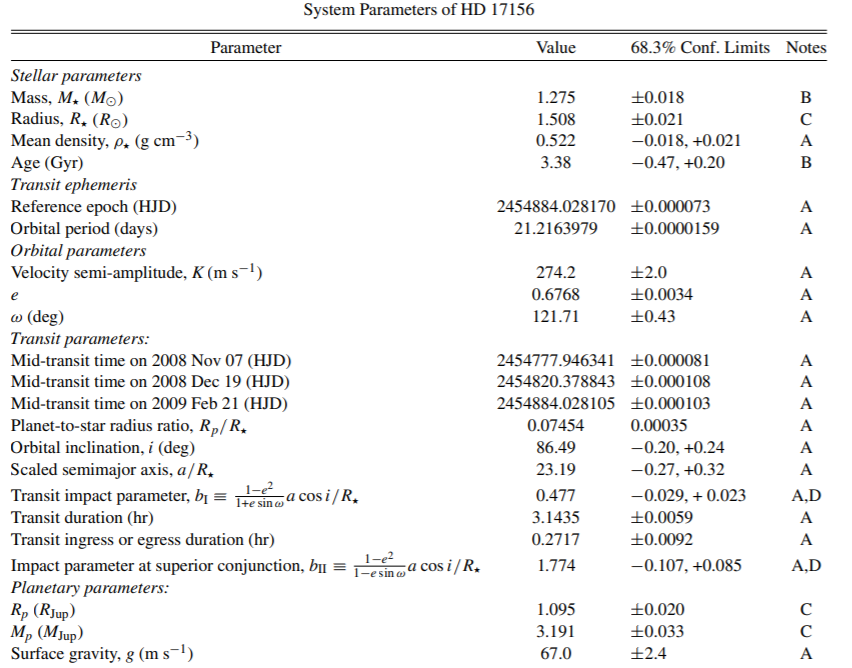
\includegraphics[width=0.6\textwidth]{../images/HD_17156.png}
	\label{Tab_1}
\end{figure}

\subsubsection*{Input Parameters}

    \begin{tcolorbox}[breakable, size=fbox, boxrule=1pt, pad at break*=1mm,colback=cellbackground, colframe=cellborder]
\prompt{In}{incolor}{6}{\boxspacing}
\begin{Verbatim}[commandchars=\\\{\}]
\PY{l+s+sd}{\PYZdq{}\PYZdq{}\PYZdq{} }
\PY{l+s+sd}{INITIAL PARAMETERS FOR HD 17156}
\PY{l+s+sd}{\PYZdq{}\PYZdq{}\PYZdq{}}

\PY{n}{HD\PYZus{}17156} \PY{o}{=} \PY{n}{Star}\PY{p}{(}\PY{l+m+mf}{1.275}\PY{p}{,} \PY{l+m+mf}{1.508}\PY{p}{)}
\PY{n}{HD\PYZus{}17156b} \PY{o}{=} \PY{n}{Planet}\PY{p}{(}\PY{n}{mass}\PY{o}{=}\PY{l+m+mf}{3.191}\PY{p}{,}
                   \PY{n}{radius}\PY{o}{=}\PY{l+m+mf}{1.095}\PY{p}{,}
                   \PY{n}{t0}\PY{o}{=}\PY{l+m+mf}{2454884.028105}\PY{p}{,}
                   \PY{n}{a}\PY{o}{=}\PY{l+m+mf}{0.1589}\PY{p}{,}
                   \PY{n}{b}\PY{o}{=}\PY{l+m+mf}{0.477}\PY{p}{,}
                   \PY{n}{e}\PY{o}{=}\PY{l+m+mf}{0.6768}\PY{p}{,}
                   \PY{n}{period}\PY{o}{=}\PY{l+m+mf}{21.2163979}\PY{p}{,}
                   \PY{n}{w}\PY{o}{=}\PY{l+m+mf}{121.71}\PY{p}{,}
                   \PY{n}{incl}\PY{o}{=}\PY{l+m+mf}{86.49}\PY{p}{)}

\PY{n}{HD\PYZus{}17156\PYZus{}system} \PY{o}{=} \PY{n}{BinarySystem}\PY{p}{(}\PY{n}{HD\PYZus{}17156}\PY{p}{,} \PY{n}{HD\PYZus{}17156b}\PY{p}{)}
\end{Verbatim}
\end{tcolorbox}

    \hypertarget{transit}{%
\subsubsection{Transit}\label{transit_1}}

    \begin{tcolorbox}[breakable, size=fbox, boxrule=1pt, pad at break*=1mm,colback=cellbackground, colframe=cellborder]
\prompt{In}{incolor}{7}{\boxspacing}
\begin{Verbatim}[commandchars=\\\{\}]
\PY{c+c1}{\PYZsh{} Plotting Dependencies }
\PY{k+kn}{import} \PY{n+nn}{matplotlib}\PY{n+nn}{.}\PY{n+nn}{pyplot} \PY{k}{as} \PY{n+nn}{plt}
\PY{n}{data} \PY{o}{=} \PY{n}{HD\PYZus{}17156\PYZus{}system}\PY{o}{.}\PY{n}{transit}\PY{p}{(}\PY{p}{)}
\PY{n}{plt}\PY{o}{.}\PY{n}{figure}\PY{p}{(}\PY{n}{figsize}\PY{o}{=}\PY{p}{(}\PY{l+m+mi}{10}\PY{p}{,} \PY{l+m+mi}{8}\PY{p}{)}\PY{p}{)}
\PY{n}{plt}\PY{o}{.}\PY{n}{scatter}\PY{p}{(}\PY{n}{data}\PY{p}{[}\PY{l+s+s2}{\PYZdq{}}\PY{l+s+s2}{timestamps}\PY{l+s+s2}{\PYZdq{}}\PY{p}{]}\PY{p}{,} \PY{n}{data}\PY{p}{[}\PY{l+s+s2}{\PYZdq{}}\PY{l+s+s2}{light\PYZus{}curve}\PY{l+s+s2}{\PYZdq{}}\PY{p}{]}\PY{p}{,} \PY{n}{marker}\PY{o}{=}\PY{l+s+s2}{\PYZdq{}}\PY{l+s+s2}{.}\PY{l+s+s2}{\PYZdq{}}\PY{p}{)}

\PY{n}{line} \PY{o}{=} \PY{n}{plt}\PY{o}{.}\PY{n}{plot}\PY{p}{(}\PY{n}{data}\PY{p}{[}\PY{l+s+s2}{\PYZdq{}}\PY{l+s+s2}{timestamps}\PY{l+s+s2}{\PYZdq{}}\PY{p}{]}\PY{p}{,} \PY{n}{data}\PY{p}{[}\PY{l+s+s2}{\PYZdq{}}\PY{l+s+s2}{light\PYZus{}curve}\PY{l+s+s2}{\PYZdq{}}\PY{p}{]}\PY{p}{)}
\PY{n}{plt}\PY{o}{.}\PY{n}{setp}\PY{p}{(}\PY{n}{line}\PY{p}{,} \PY{n}{linewidth}\PY{o}{=}\PY{l+m+mi}{1}\PY{p}{,} \PY{n}{linestyle}\PY{o}{=}\PY{l+s+s2}{\PYZdq{}}\PY{l+s+s2}{\PYZhy{}\PYZhy{}}\PY{l+s+s2}{\PYZdq{}}\PY{p}{)}
\PY{n}{plt}\PY{o}{.}\PY{n}{title}\PY{p}{(}\PY{l+s+s2}{\PYZdq{}}\PY{l+s+s2}{Transit Light Curve for HD 17156}\PY{l+s+s2}{\PYZdq{}}\PY{p}{)}
\PY{n}{plt}\PY{o}{.}\PY{n}{xlabel}\PY{p}{(}\PY{l+s+s2}{\PYZdq{}}\PY{l+s+s2}{Period/days}\PY{l+s+s2}{\PYZdq{}}\PY{p}{)}
\PY{n}{plt}\PY{o}{.}\PY{n}{ylabel}\PY{p}{(}\PY{l+s+s2}{\PYZdq{}}\PY{l+s+s2}{Normalised Flux}\PY{l+s+s2}{\PYZdq{}}\PY{p}{)}
\PY{n}{plt}\PY{o}{.}\PY{n}{grid}\PY{p}{(}\PY{k+kc}{True}\PY{p}{)}
\PY{n}{plt}\PY{o}{.}\PY{n}{show}\PY{p}{(}\PY{p}{)}
\end{Verbatim}
\end{tcolorbox}

\begin{figure}[!hbt]
	\figuretitle{Output:}
	\centering
	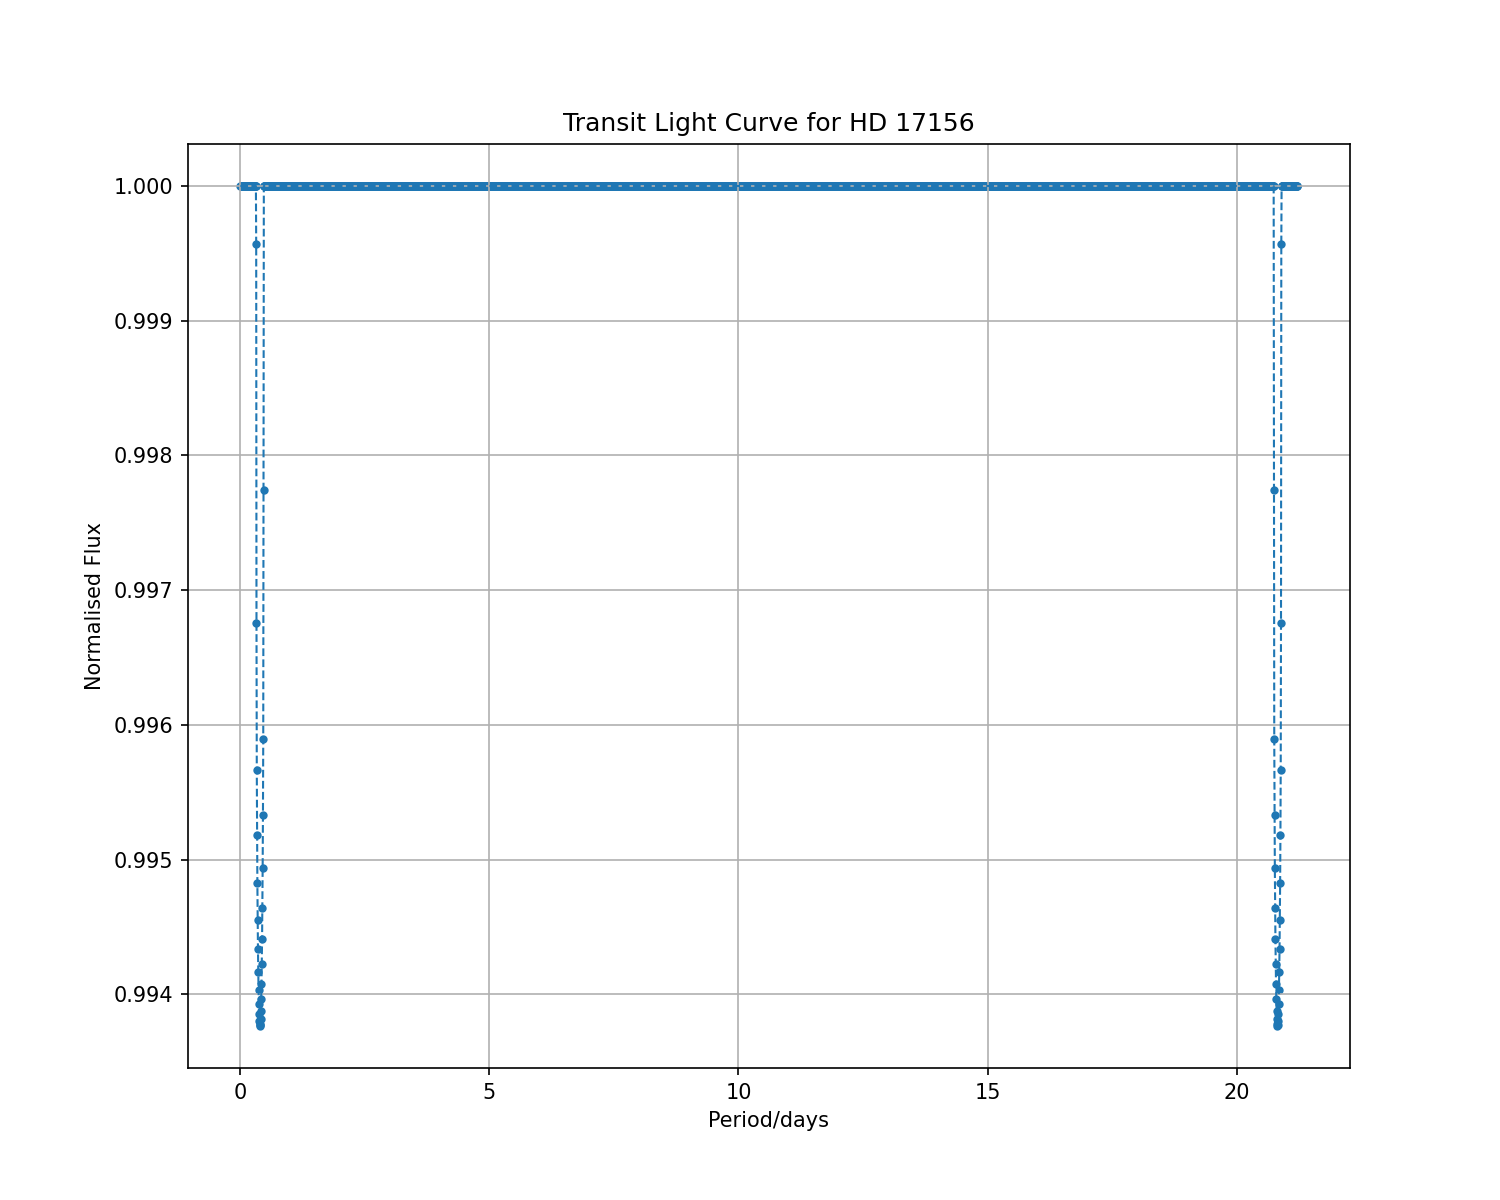
\includegraphics[width=0.75\textwidth]{../matplotlib_graphs/transit_1.png}
\end{figure}    


\begin{figure}[!h]
	\centering 
	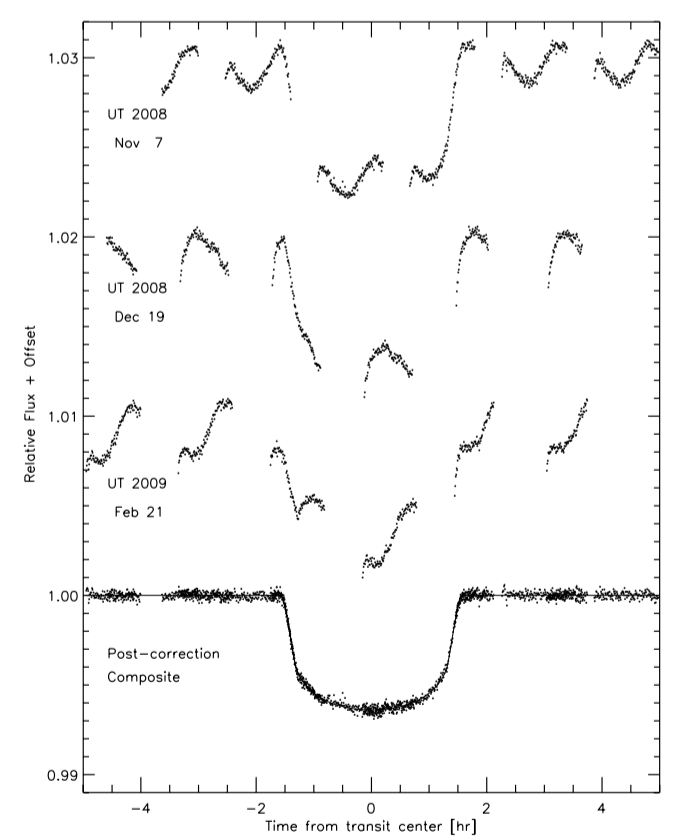
\includegraphics[width=0.41\textwidth]{../images/light_curve.png}
	\caption{Figure showing the light curve of HD 17156 measured by Nutzman et al. (2010).} 
	\label{Figure 4.a}
\end{figure}

    \hypertarget{observations}{%
\paragraph{Observations}\label{observations_1}}

When compared to the light curve measured by Nutzmann et al., we note
that the light curve we produce is very similar: it can be observed that the total, full and ingress/egress duration of the transit (see \ref{the-light-curve}) is almost identical- around 3 hours for the full transit time- when we convert period from days to hours. The depth of the transit curve, \(\delta\), is also concurrent with the measured results, just under 0.994.


    \hypertarget{radial-velocity}{%
\subsubsection{Radial Velocity}\label{radial-velocity_1}}

    \begin{tcolorbox}[breakable, size=fbox, boxrule=1pt, pad at break*=1mm,colback=cellbackground, colframe=cellborder]
\prompt{In}{incolor}{8}{\boxspacing}
\begin{Verbatim}[commandchars=\\\{\}]
\PY{c+c1}{\PYZsh{} Plotting Dependencies }
\PY{k+kn}{import} \PY{n+nn}{matplotlib}\PY{n+nn}{.}\PY{n+nn}{pyplot} \PY{k}{as} \PY{n+nn}{plt}

\PY{n}{data} \PY{o}{=} \PY{n}{HD\PYZus{}17156\PYZus{}system}\PY{o}{.}\PY{n}{radial\PYZus{}velocity}\PY{p}{(}\PY{p}{)}

\PY{n}{plt}\PY{o}{.}\PY{n}{figure}\PY{p}{(}\PY{n}{figsize}\PY{o}{=}\PY{p}{(}\PY{l+m+mi}{10}\PY{p}{,} \PY{l+m+mi}{8}\PY{p}{)}\PY{p}{)}
\PY{n}{plt}\PY{o}{.}\PY{n}{scatter}\PY{p}{(}\PY{n}{data}\PY{p}{[}\PY{l+s+s2}{\PYZdq{}}\PY{l+s+s2}{timestamps}\PY{l+s+s2}{\PYZdq{}}\PY{p}{]}\PY{p}{,} \PY{n}{data}\PY{p}{[}\PY{l+s+s2}{\PYZdq{}}\PY{l+s+s2}{radial\PYZus{}velocity}\PY{l+s+s2}{\PYZdq{}}\PY{p}{]}\PY{p}{,} \PY{n}{marker} \PY{o}{=} \PY{l+s+s2}{\PYZdq{}}\PY{l+s+s2}{.}\PY{l+s+s2}{\PYZdq{}}\PY{p}{)}

\PY{n}{line} \PY{o}{=} \PY{n}{plt}\PY{o}{.}\PY{n}{plot}\PY{p}{(}\PY{n}{data}\PY{p}{[}\PY{l+s+s2}{\PYZdq{}}\PY{l+s+s2}{timestamps}\PY{l+s+s2}{\PYZdq{}}\PY{p}{]}\PY{p}{,} \PY{n}{data}\PY{p}{[}\PY{l+s+s2}{\PYZdq{}}\PY{l+s+s2}{radial\PYZus{}velocity}\PY{l+s+s2}{\PYZdq{}}\PY{p}{]}\PY{p}{)}
\PY{n}{plt}\PY{o}{.}\PY{n}{setp}\PY{p}{(}\PY{n}{line}\PY{p}{,} \PY{n}{linewidth}\PY{o}{=}\PY{l+m+mi}{1}\PY{p}{,} \PY{n}{linestyle}\PY{o}{=}\PY{l+s+s2}{\PYZdq{}}\PY{l+s+s2}{\PYZhy{}\PYZhy{}}\PY{l+s+s2}{\PYZdq{}}\PY{p}{)}

\PY{n}{plt}\PY{o}{.}\PY{n}{title}\PY{p}{(}\PY{l+s+s2}{\PYZdq{}}\PY{l+s+s2}{Radial Velocity for HD 17156}\PY{l+s+s2}{\PYZdq{}}\PY{p}{)}
\PY{n}{plt}\PY{o}{.}\PY{n}{xlabel}\PY{p}{(}\PY{l+s+s2}{\PYZdq{}}\PY{l+s+s2}{Period/days}\PY{l+s+s2}{\PYZdq{}}\PY{p}{)}
\PY{n}{plt}\PY{o}{.}\PY{n}{ylabel}\PY{p}{(}\PY{l+s+s2}{\PYZdq{}}\PY{l+s+s2}{Velocity/AU*day\PYZca{}\PYZhy{}1}\PY{l+s+s2}{\PYZdq{}}\PY{p}{)}
\PY{n}{plt}\PY{o}{.}\PY{n}{grid}\PY{p}{(}\PY{k+kc}{True}\PY{p}{)}
\PY{n}{plt}\PY{o}{.}\PY{n}{show}\PY{p}{(}\PY{p}{)}
\end{Verbatim}
\end{tcolorbox}

\begin{figure}[H]
	\figuretitle{Output:}
	\centering
	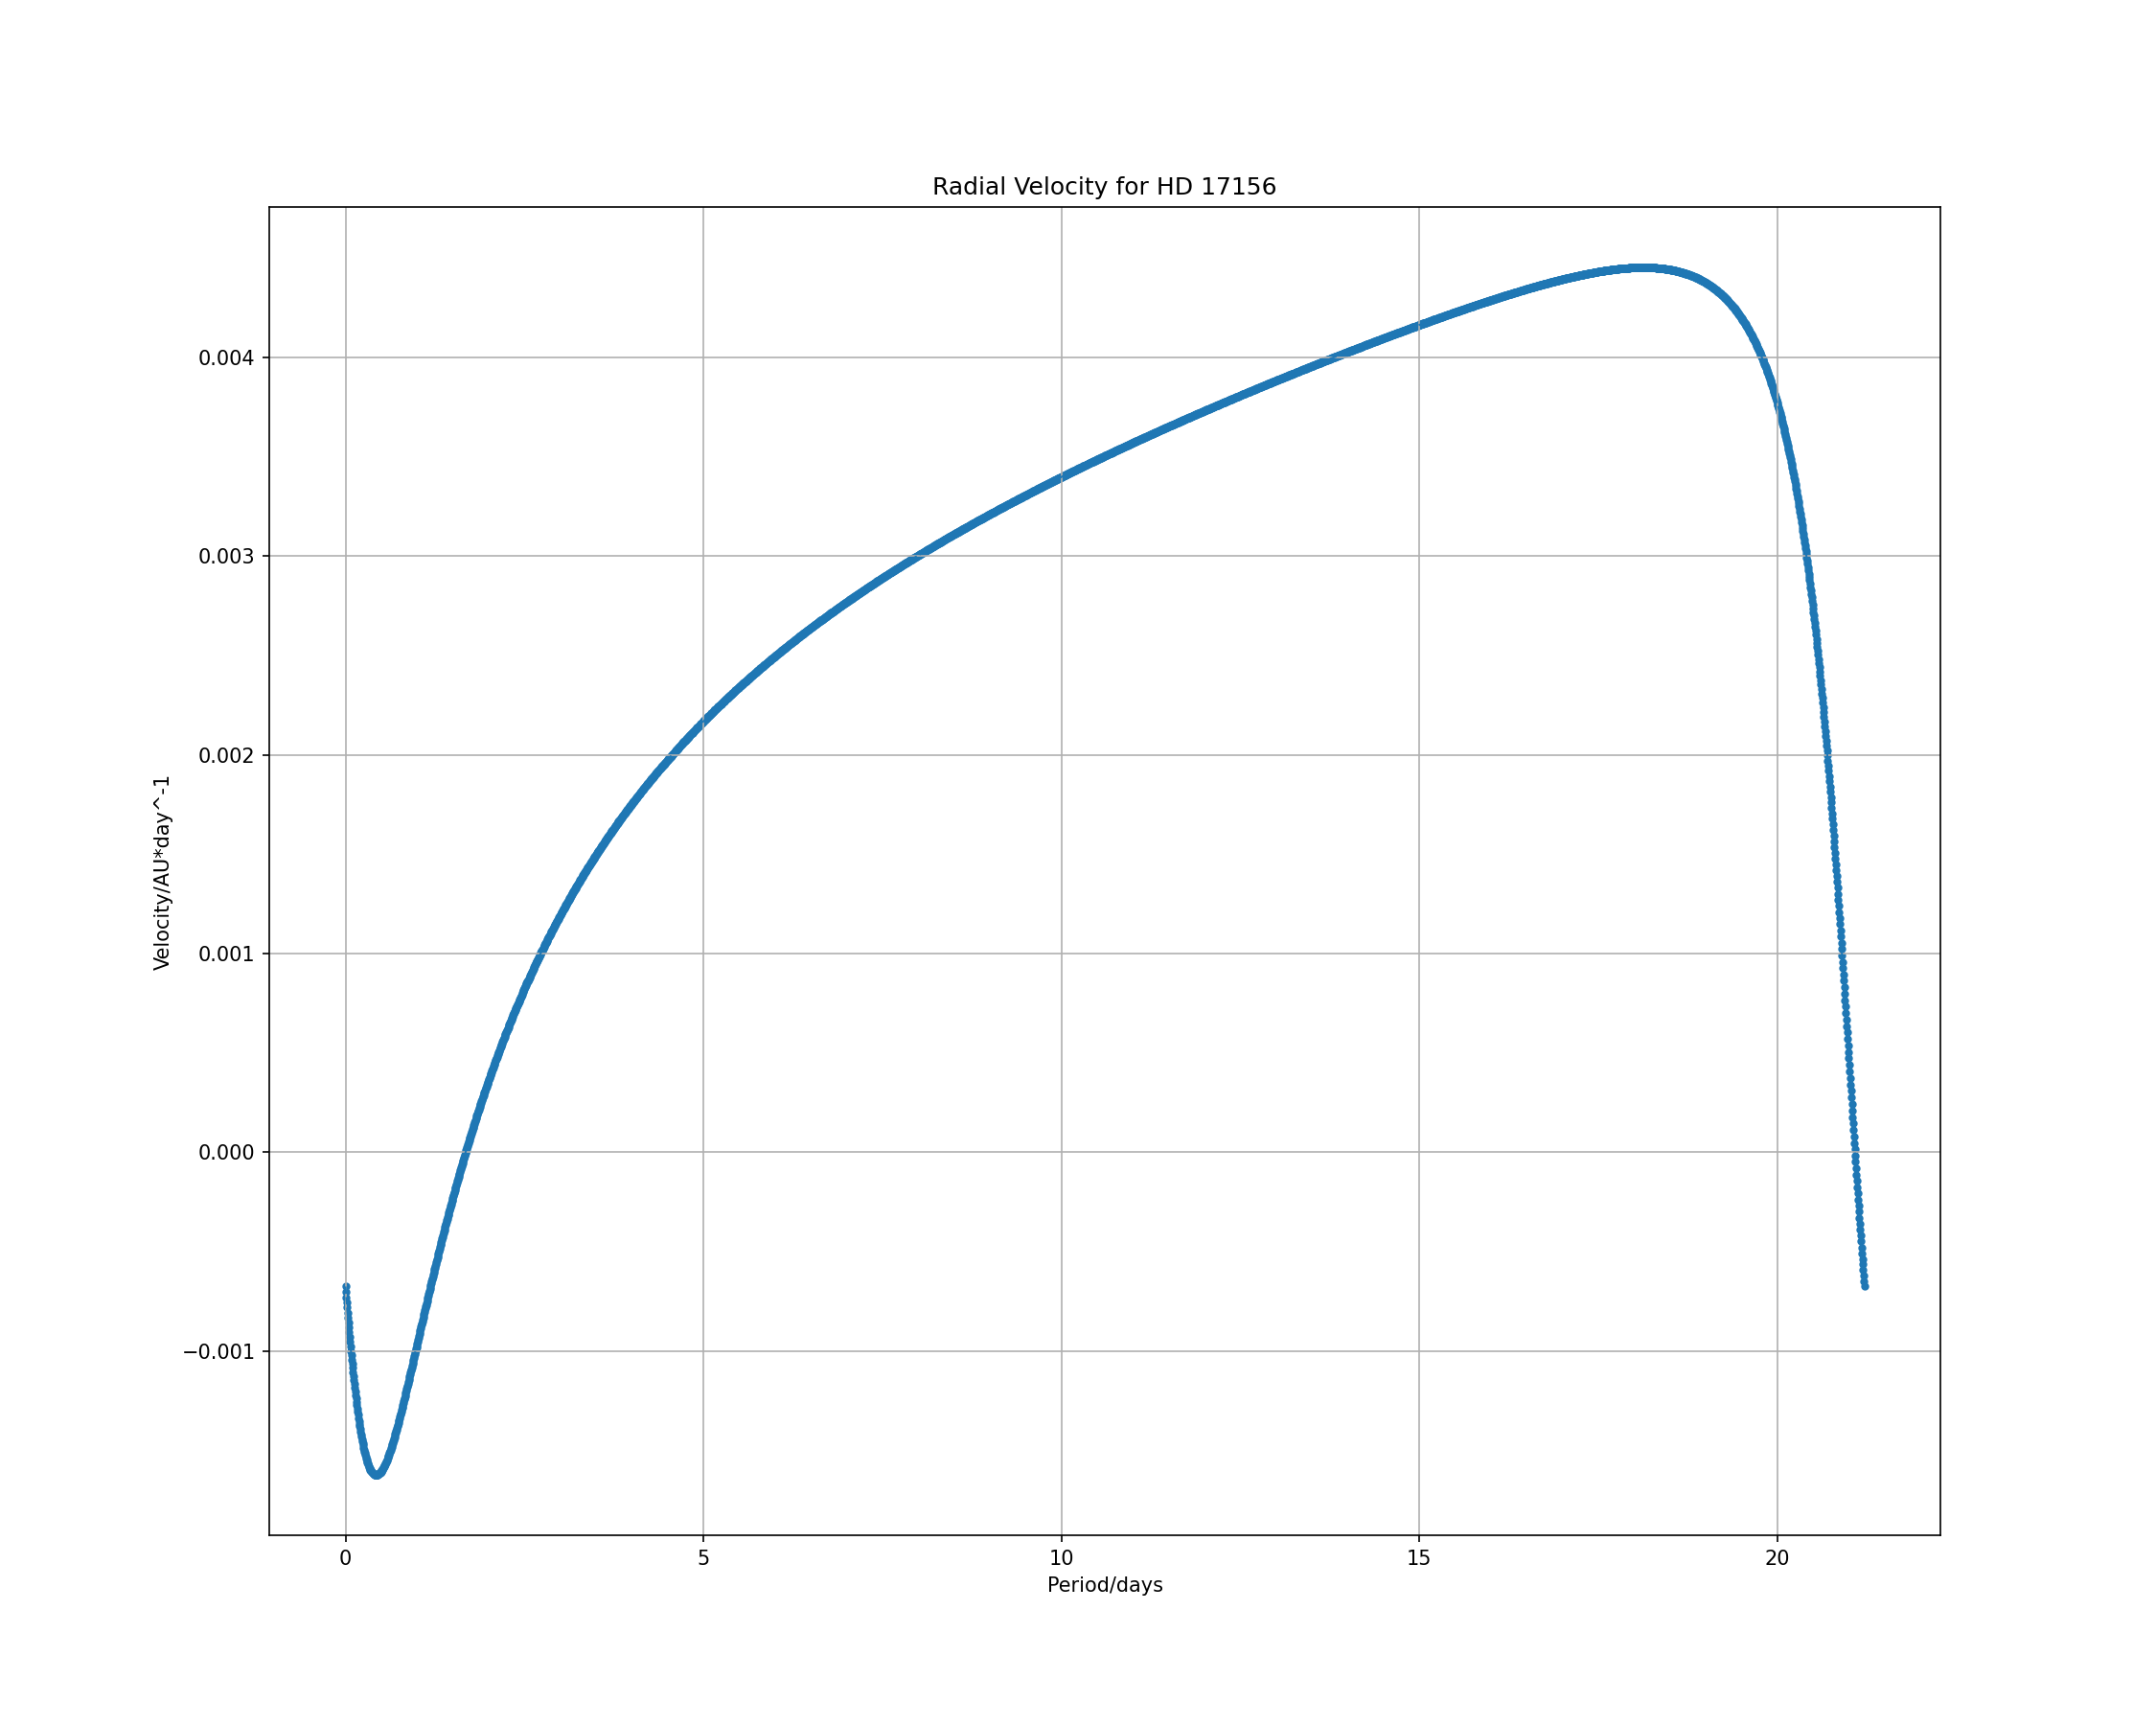
\includegraphics[width=0.75\textwidth]{../matplotlib_graphs/radial_velocity_1.png}
\end{figure} 
    

\begin{figure}[!hbt]
	\centering 
	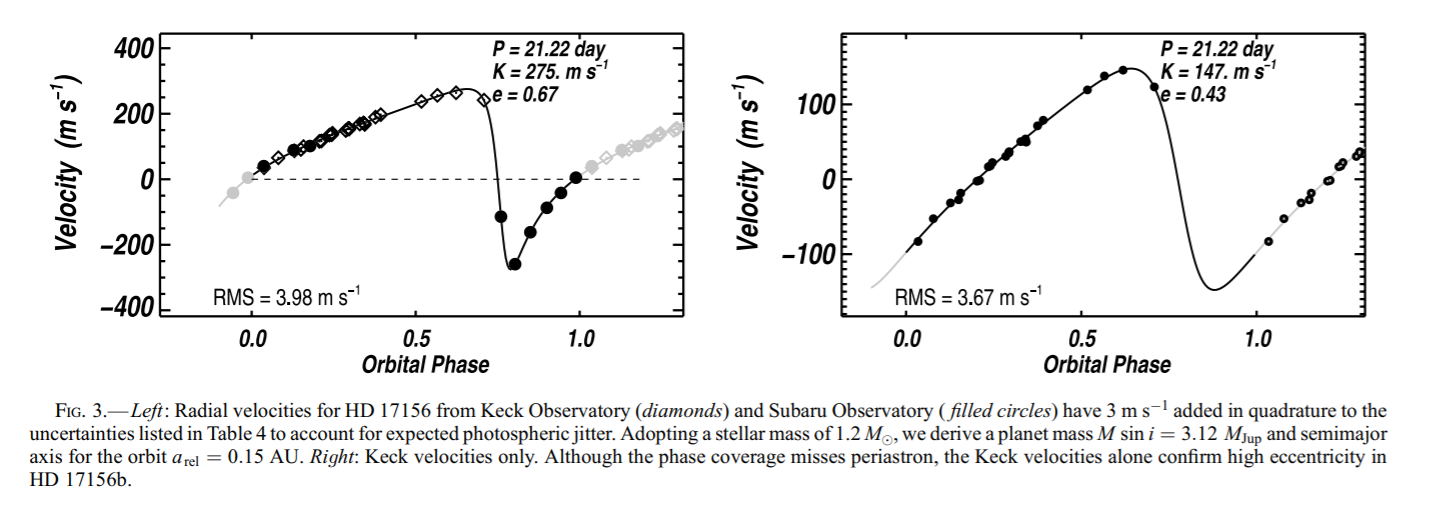
\includegraphics[width=\textwidth]{../images/radial_v_graph.png}
	\caption{{\it Left}: Radial velocities for HD 17156 from the Keck Observatory ({\it diamonds}) and Subaru Observatory ({\it filled circles}) accounting for uncertainties caused by photospheric jitter. {\it Right}: Keck velocities only. Although the phase coverage misses periastron, the Keck velocities alone confirm high eccentricity in HD 17156b. Fisher et al. (2007).} 
	\label{Figure 4.b}
\end{figure}



    \hypertarget{observations}{%
\paragraph{Observations}\label{observations_2}}

We note that our radial velocity variations are 0.6 of the orbital phase out with Fisher's results; otherwise the results on the graph seem to be of similar proportion and shape. Once converted, the semi-amplitude of our graph, \(K\), is concurrent with the results above.


\hypertarget{tres-3}{%
\subsection{TrES-3}\label{tres-3}}

Orbiting the star GSC 03089-00929, 760 light-years away in the
constellation of Hercules, TrES-3b is an extrasolar planet that has an
orbital period of just 31 hours and has nearly twice the mass of
Jupiter. Below is a figure containing all the initial parameters for TrES-3 as measured by Sozzetti et al. (2009).

\begin{figure}
	\centering
	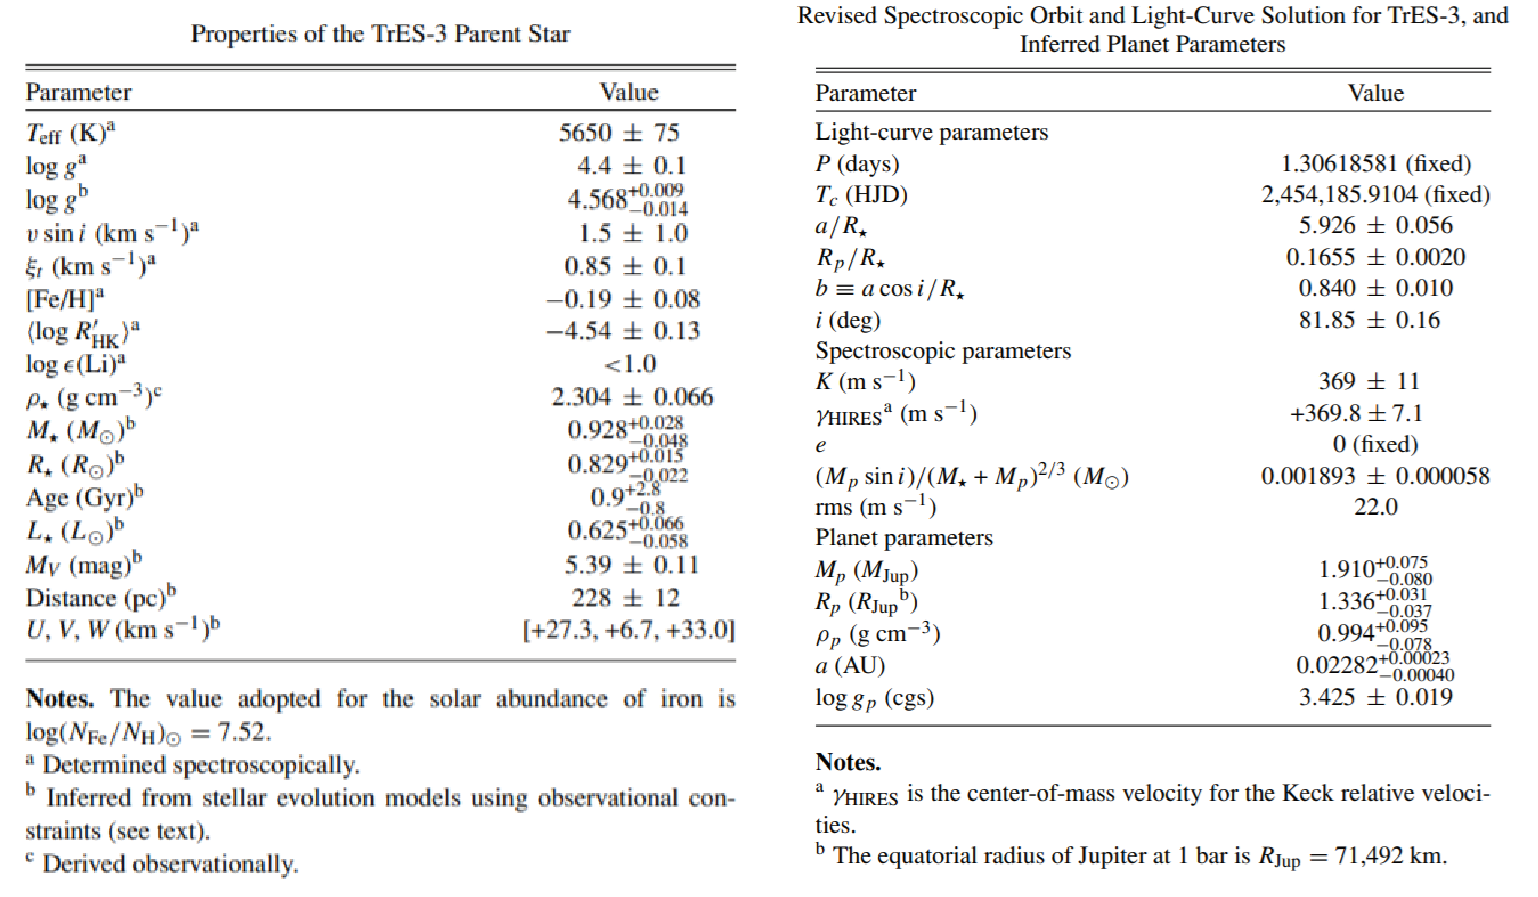
\includegraphics[width=1\linewidth]{../images/TrES-3_combined.png}
	\label{Tab 2}
\end{figure}

\medskip

\subsubsection*{Input Parameters}


    \begin{tcolorbox}[breakable, size=fbox, boxrule=1pt, pad at break*=1mm,colback=cellbackground, colframe=cellborder]
\prompt{In}{incolor}{9}{\boxspacing}
\begin{Verbatim}[commandchars=\\\{\}]
\PY{l+s+sd}{\PYZdq{}\PYZdq{}\PYZdq{} }
\PY{l+s+sd}{INITIAL PARAMETERS FOR TrES\PYZhy{}3}
\PY{l+s+sd}{\PYZdq{}\PYZdq{}\PYZdq{}}

\PY{n}{TrES\PYZus{}3} \PY{o}{=} \PY{n}{Star}\PY{p}{(}\PY{l+m+mf}{0.928}\PY{p}{,} \PY{l+m+mf}{0.829}\PY{p}{)}
\PY{n}{TrES\PYZus{}3b} \PY{o}{=} \PY{n}{Planet}\PY{p}{(}\PY{n}{mass}\PY{o}{=}\PY{l+m+mf}{1.910}\PY{p}{,}
                   \PY{n}{radius}\PY{o}{=}\PY{l+m+mf}{1.336}\PY{p}{,}
                   \PY{n}{t0}\PY{o}{=}\PY{l+m+mf}{2454532.04939}\PY{p}{,}
                   \PY{n}{a}\PY{o}{=}\PY{l+m+mf}{0.02282}\PY{p}{,}
                   \PY{n}{b}\PY{o}{=}\PY{l+m+mf}{0.840}\PY{p}{,}
                   \PY{n}{e}\PY{o}{=}\PY{l+m+mi}{0}\PY{p}{,}
                   \PY{n}{period}\PY{o}{=}\PY{l+m+mf}{1.306186581}\PY{p}{,}
                   \PY{n}{w}\PY{o}{=}\PY{l+m+mi}{0}\PY{p}{,}
                   \PY{n}{incl}\PY{o}{=}\PY{l+m+mf}{81.85}\PY{p}{)}



\PY{n}{TrES\PYZus{}3\PYZus{}system} \PY{o}{=} \PY{n}{BinarySystem}\PY{p}{(}\PY{n}{TrES\PYZus{}3}\PY{p}{,} \PY{n}{TrES\PYZus{}3b}\PY{p}{)}
\end{Verbatim}
\end{tcolorbox}

    \hypertarget{transit}{%
\subsubsection{Transit}\label{transit_2}}

    \begin{tcolorbox}[breakable, size=fbox, boxrule=1pt, pad at break*=1mm,colback=cellbackground, colframe=cellborder]
\prompt{In}{incolor}{10}{\boxspacing}
\begin{Verbatim}[commandchars=\\\{\}]
\PY{c+c1}{\PYZsh{} Plotting Dependencies }
\PY{k+kn}{import} \PY{n+nn}{matplotlib}\PY{n+nn}{.}\PY{n+nn}{pyplot} \PY{k}{as} \PY{n+nn}{plt}

\PY{n}{data} \PY{o}{=} \PY{n}{TrES\PYZus{}3\PYZus{}system}\PY{o}{.}\PY{n}{transit}\PY{p}{(}\PY{p}{)}

\PY{n}{plt}\PY{o}{.}\PY{n}{figure}\PY{p}{(}\PY{n}{figsize}\PY{o}{=}\PY{p}{(}\PY{l+m+mi}{10}\PY{p}{,} \PY{l+m+mi}{8}\PY{p}{)}\PY{p}{)}
\PY{n}{plt}\PY{o}{.}\PY{n}{scatter}\PY{p}{(}\PY{n}{data}\PY{p}{[}\PY{l+s+s2}{\PYZdq{}}\PY{l+s+s2}{timestamps}\PY{l+s+s2}{\PYZdq{}}\PY{p}{]}\PY{p}{,} \PY{n}{data}\PY{p}{[}\PY{l+s+s2}{\PYZdq{}}\PY{l+s+s2}{light\PYZus{}curve}\PY{l+s+s2}{\PYZdq{}}\PY{p}{]}\PY{p}{,} \PY{n}{marker}\PY{o}{=}\PY{l+s+s2}{\PYZdq{}}\PY{l+s+s2}{.}\PY{l+s+s2}{\PYZdq{}}\PY{p}{)}

\PY{n}{line} \PY{o}{=} \PY{n}{plt}\PY{o}{.}\PY{n}{plot}\PY{p}{(}\PY{n}{data}\PY{p}{[}\PY{l+s+s2}{\PYZdq{}}\PY{l+s+s2}{timestamps}\PY{l+s+s2}{\PYZdq{}}\PY{p}{]}\PY{p}{,} \PY{n}{data}\PY{p}{[}\PY{l+s+s2}{\PYZdq{}}\PY{l+s+s2}{light\PYZus{}curve}\PY{l+s+s2}{\PYZdq{}}\PY{p}{]}\PY{p}{)}
\PY{n}{plt}\PY{o}{.}\PY{n}{setp}\PY{p}{(}\PY{n}{line}\PY{p}{,} \PY{n}{linewidth}\PY{o}{=}\PY{l+m+mi}{1}\PY{p}{,} \PY{n}{linestyle}\PY{o}{=}\PY{l+s+s2}{\PYZdq{}}\PY{l+s+s2}{\PYZhy{}\PYZhy{}}\PY{l+s+s2}{\PYZdq{}}\PY{p}{)}

\PY{n}{plt}\PY{o}{.}\PY{n}{title}\PY{p}{(}\PY{l+s+s2}{\PYZdq{}}\PY{l+s+s2}{Transit Light Curve for TrES\PYZhy{}3}\PY{l+s+s2}{\PYZdq{}}\PY{p}{)}
    
\PY{n}{plt}\PY{o}{.}\PY{n}{xlabel}\PY{p}{(}\PY{l+s+s2}{\PYZdq{}}\PY{l+s+s2}{Period/days}\PY{l+s+s2}{\PYZdq{}}\PY{p}{)}
\PY{n}{plt}\PY{o}{.}\PY{n}{ylabel}\PY{p}{(}\PY{l+s+s2}{\PYZdq{}}\PY{l+s+s2}{Normalised Flux}\PY{l+s+s2}{\PYZdq{}}\PY{p}{)}
\PY{n}{plt}\PY{o}{.}\PY{n}{grid}\PY{p}{(}\PY{k+kc}{True}\PY{p}{)}
\PY{n}{plt}\PY{o}{.}\PY{n}{show}\PY{p}{(}\PY{p}{)}
\end{Verbatim}
\end{tcolorbox}

    
\begin{figure}[!hbt]
	\figuretitle{Output:}
	\centering
	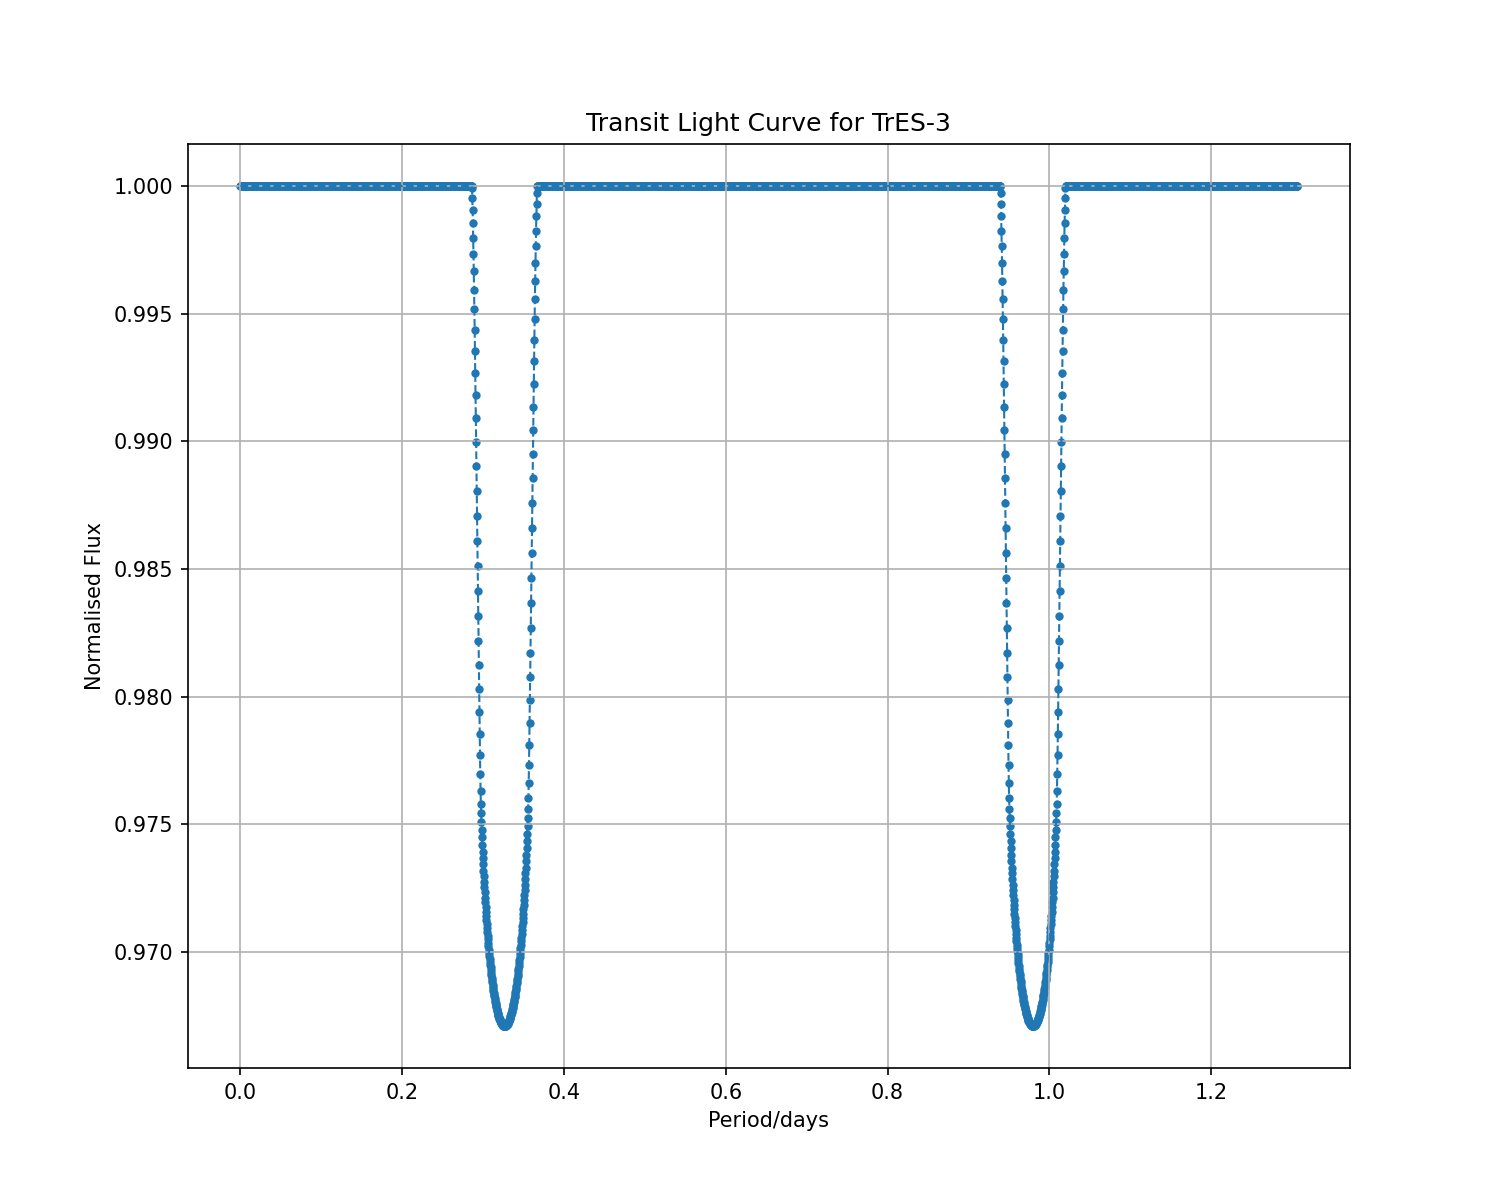
\includegraphics[width=0.75\textwidth]{../matplotlib_graphs/transit_2.png}
\end{figure} 


\begin{figure}[!hbt]
	\centering
	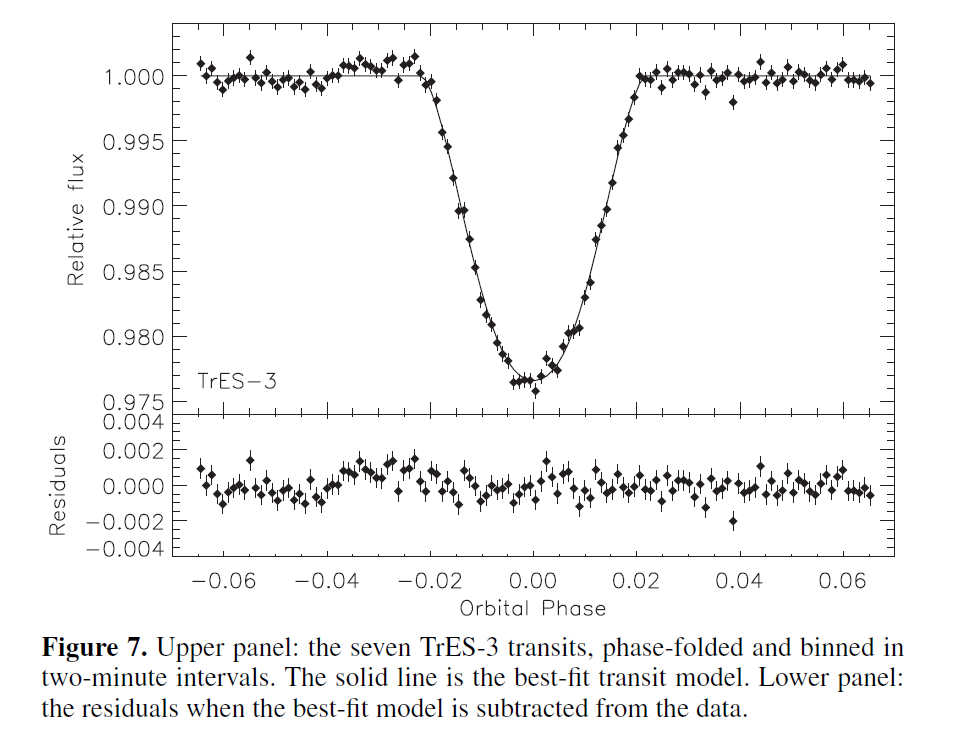
\includegraphics[width=0.75\textwidth]{../images/TrE-S_light_curve.png}
	\caption{The transit light curve as measured by Christiansen et al. (2007). {\it Upper panel}: The seven TrES-3 transits, phase-folded and binned in two-minute intervals. The solid line is the best-fit transit model. {\it Lower panel}: the residuals when the best-fit model is subtracted from the data.} 
	\label{Figure 4.c}
\end{figure}



    \hypertarget{observations}{%
\paragraph{Observations}\label{observations_3}}

As regards to the total, full and ingress/egress duration of the transit
(see 2.5), we note that our model produces results that are fairly
accurate. \(\delta\), however, seems to be slightly too large in our
calculations- around 0.968 as opposed to 0.976 as measured by
Christiansen et al.- which suggests that the input data has fairly large degrees of uncertainty.


    \hypertarget{radial-velocity}{%
\subsubsection{Radial Velocity}\label{radial-velocity_2}}

    \begin{tcolorbox}[breakable, size=fbox, boxrule=1pt, pad at break*=1mm,colback=cellbackground, colframe=cellborder]
\prompt{In}{incolor}{11}{\boxspacing}
\begin{Verbatim}[commandchars=\\\{\}]
\PY{c+c1}{\PYZsh{} Plotting Dependencies }
\PY{k+kn}{import} \PY{n+nn}{matplotlib}\PY{n+nn}{.}\PY{n+nn}{pyplot} \PY{k}{as} \PY{n+nn}{plt}

\PY{n}{data} \PY{o}{=} \PY{n}{TrES\PYZus{}3\PYZus{}system}\PY{o}{.}\PY{n}{radial\PYZus{}velocity}\PY{p}{(}\PY{p}{)}

\PY{n}{plt}\PY{o}{.}\PY{n}{figure}\PY{p}{(}\PY{n}{figsize}\PY{o}{=}\PY{p}{(}\PY{l+m+mi}{10}\PY{p}{,} \PY{l+m+mi}{8}\PY{p}{)}\PY{p}{)}
\PY{n}{plt}\PY{o}{.}\PY{n}{scatter}\PY{p}{(}\PY{n}{data}\PY{p}{[}\PY{l+s+s2}{\PYZdq{}}\PY{l+s+s2}{timestamps}\PY{l+s+s2}{\PYZdq{}}\PY{p}{]}\PY{p}{,} \PY{n}{data}\PY{p}{[}\PY{l+s+s2}{\PYZdq{}}\PY{l+s+s2}{radial\PYZus{}velocity}\PY{l+s+s2}{\PYZdq{}}\PY{p}{]}\PY{p}{,} \PY{n}{marker} \PY{o}{=} \PY{l+s+s2}{\PYZdq{}}\PY{l+s+s2}{.}\PY{l+s+s2}{\PYZdq{}}\PY{p}{)}

\PY{n}{line} \PY{o}{=} \PY{n}{plt}\PY{o}{.}\PY{n}{plot}\PY{p}{(}\PY{n}{data}\PY{p}{[}\PY{l+s+s2}{\PYZdq{}}\PY{l+s+s2}{timestamps}\PY{l+s+s2}{\PYZdq{}}\PY{p}{]}\PY{p}{,} \PY{n}{data}\PY{p}{[}\PY{l+s+s2}{\PYZdq{}}\PY{l+s+s2}{radial\PYZus{}velocity}\PY{l+s+s2}{\PYZdq{}}\PY{p}{]}\PY{p}{)}
\PY{n}{plt}\PY{o}{.}\PY{n}{setp}\PY{p}{(}\PY{n}{line}\PY{p}{,} \PY{n}{linewidth}\PY{o}{=}\PY{l+m+mi}{1}\PY{p}{,} \PY{n}{linestyle}\PY{o}{=}\PY{l+s+s2}{\PYZdq{}}\PY{l+s+s2}{\PYZhy{}\PYZhy{}}\PY{l+s+s2}{\PYZdq{}}\PY{p}{)}

\PY{n}{plt}\PY{o}{.}\PY{n}{title}\PY{p}{(}\PY{l+s+s2}{\PYZdq{}}\PY{l+s+s2}{Radial Velocity for TrES\PYZhy{}3}\PY{l+s+s2}{\PYZdq{}}\PY{p}{)}
    
\PY{n}{plt}\PY{o}{.}\PY{n}{xlabel}\PY{p}{(}\PY{l+s+s2}{\PYZdq{}}\PY{l+s+s2}{Period/days}\PY{l+s+s2}{\PYZdq{}}\PY{p}{)}
\PY{n}{plt}\PY{o}{.}\PY{n}{ylabel}\PY{p}{(}\PY{l+s+s2}{\PYZdq{}}\PY{l+s+s2}{Velocity/AU*day\PYZca{}\PYZhy{}1}\PY{l+s+s2}{\PYZdq{}}\PY{p}{)}

\PY{n}{plt}\PY{o}{.}\PY{n}{grid}\PY{p}{(}\PY{k+kc}{True}\PY{p}{)}
\PY{n}{plt}\PY{o}{.}\PY{n}{show}\PY{p}{(}\PY{p}{)}
\end{Verbatim}
\end{tcolorbox}


\begin{figure}[!hbt]
	\figuretitle{Output:}
	\centering
	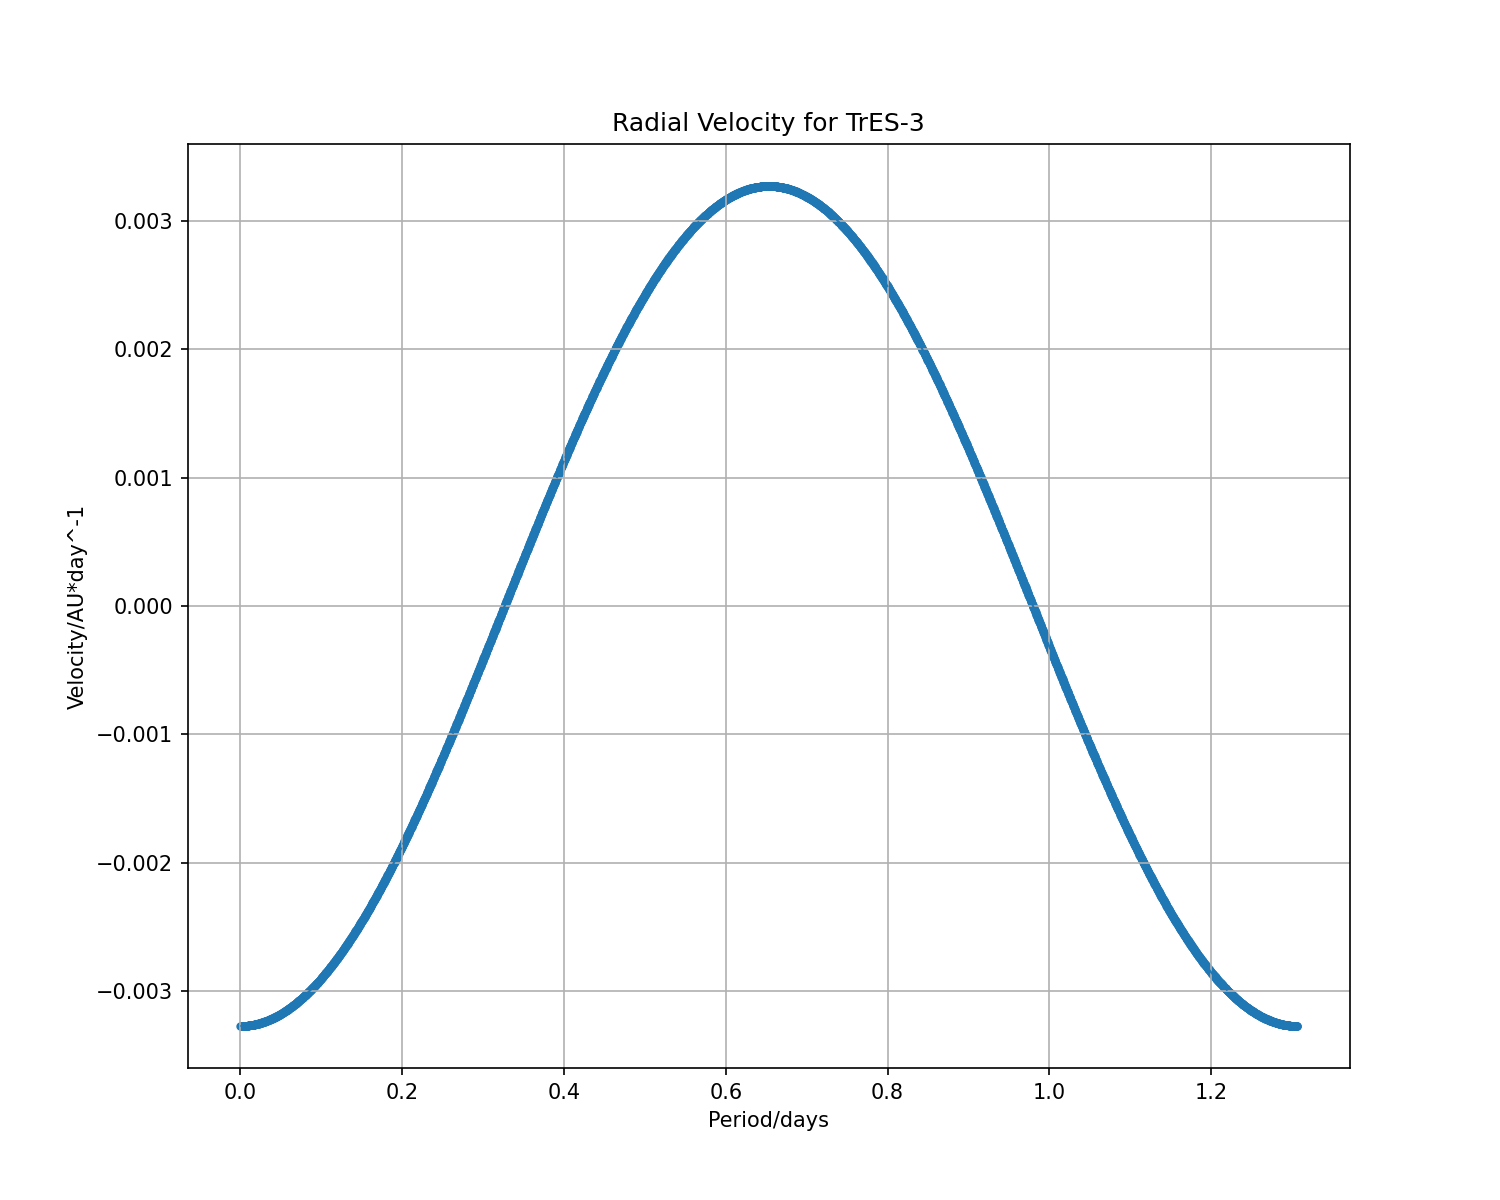
\includegraphics[width=0.75\textwidth]{../matplotlib_graphs/radial_velocity_2.png}
\end{figure} 

    
\begin{figure}[!hbt]
	\centering
	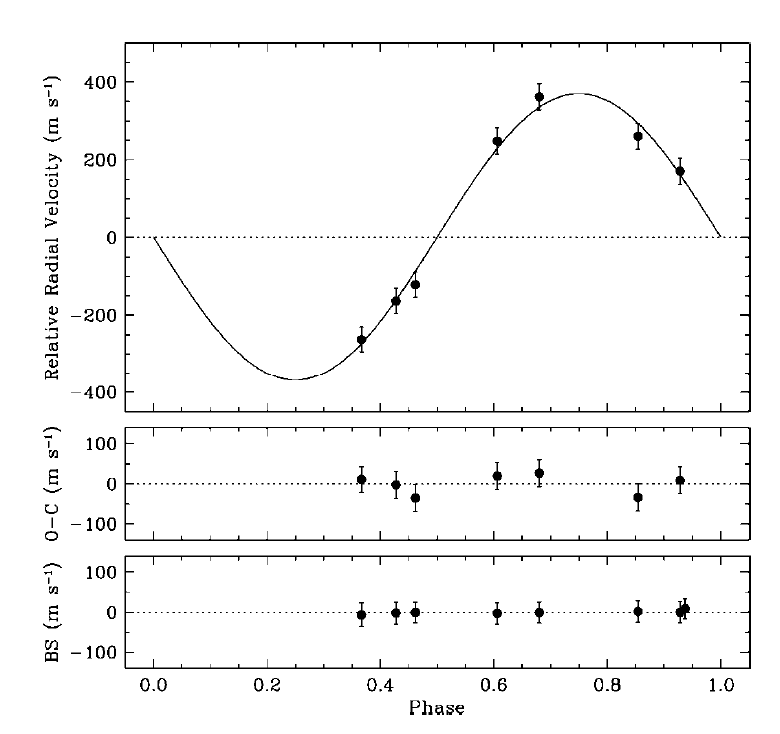
\includegraphics[width=0.7\textwidth]{../images/TrE-S_radial_velocity.png}
	\caption{{\it Top}: Radial velocity observations of TrES-3 obtained with Keck/HIRES using a $I_{2}$ cell, shown relative to the centre of mass. The best-fit model ({\it solid line}) is overplotted. {\it Middle}: Residuals from the best-fit model to the radial velocities. {\it Bottom}: Bisector spans shifted to a median of zero, for each of the iodine exposures as well as for the template (which is shown as the additional data point at phase 0.937). O'Donovan et al. (2007).} \label{Figure 4.d}
\end{figure}    


    \hypertarget{observations}{%
\paragraph{Observations}\label{observations_4}}

A smooth curve: the shape and size of our results seem to be accurate.
We note that our radial velocity variations are 0.2 of the orbital phase
out with O'Donovan's results, suggesting error in our initial parameters
or a logical error with the model.\\

\begin{center}\rule{0.5\linewidth}{0.5pt}\end{center}

    \hypertarget{conclusion}{%
\section{Conclusion}\label{conclusion}}



As a Keplerian model of a binary exoplanet system, this model achieves
the aims listed in \ref{fundamental-aims}: we have created a program that models an exoplanet system to produce predictions for observations from Earth, which can be applied to any known binary exoplanet system. These predictions have been compared with actual data, producing realistic quantitative results that can be tested against real astronomical data.

\hypertarget{limitations}{%
\subsection{Limitations}\label{limitations}}

Certain numerical calculations mean that the model has a limited
accuracy when predicting the light curve, accounting for some of the
errors seen in section 4. The speed of the model, although reasonably
fast, could be made quicker through optimising some of the numerical
calculation processes, such as the integration of the light curve; use
of the timeit module could have useful applications.

Whilst the light curve appears to be reasonably accurate, we note that
the radial velocity method does not account for the Rossiter--McLaughlin
effect, a spectroscopic phenomenon observed as the main star rotates on
its axis: the rotation of the star produces shifts in the stellar
spectra. When the exoplanet transits the star, some of the shifted light
is blocked, causing the observed mean redshift of the primary star to
vary from its normal value. As the exoplanet moves across the transit,
the redshift anomaly will switch from being negative to being positive,
or vice versa. This will be a key area of development for the future,
especially since this effect appears to be commonplace amongst Hot
Jupiters.

\hypertarget{future-development}{%
\subsection{Future Development}\label{future-development}}

With the promise of larger telescopes in the near future, larger
collecting areas will produce more focused and accurate readings,
facilitating the further expansion of the model with more accurate data.
However, these will encounter challenges that will limit the improvement
in measurement precision: the solution to these limiting factors, if
any, will most likely be in the development of new data processing and
analysis techniques.

The future expansion of the capabilities offered by this project would
be to apply it to an N-body problem. In terms of software development,
improvements would be focused on refining the accuracy of the model and
correcting the anomalies described above. The final stage would be to
connect these results to a data base, through the use of SQL, allowing
the quick access of data produced by this model.

\newpage

\begin{center}\rule{0.5\linewidth}{0.5pt}\end{center}

\hypertarget{references}{%
\section*{{Bibliography}}\label{references}}

Christiansen, J.L. et al., 2010. \textit{System parameters, transit
times, and secondary eclipse constraints of the exoplanet systems
HAT-P-4, TrES-2, TrES-3, and WASP-3 from the NASA EPOXI mission of
opportunity.} The Astrophysical Journal, 726(2), p.94.

Fischer, D.A. et al., 2011. \textit{Radial Velocity Techniques for Exoplanets}; University of Arizona Press: Tucson, AZ, USA.

Lovis, C. and Fischer, D., 2010. \textit{Radial velocity techniques for
exoplanets.} Exoplanets, pp.27-53.

Nutzman, P. et al., 2010. \textit{Precise estimates of the physical parameters for the exoplanet system HD 17156 enabled by Hubble Space Telescope fine guidance sensor transit and asteroseismic observations.} The Astrophysical Journal, 726(1), p.3.

Perryman, M., 2018. \textit{The exoplanet handbook.} Cambridge University Press. Retrieved 10 Feb, 2020, from
http://exoplanet.eu/media/flatpages\_documents/20180101-macp-detection-methods-color.pdf

Reed, B.C., 2019. \textit{Keplerian Ellipses: The Physics of the Gravitational Two-body Problem.} Morgan \& Claypool Publishers. p.6-1

Schneider, J. \textit{Interactive Extra-solar Planets Catalog.} The
Extrasolar Planets Encyclopedia. Retrieved 5 February 2020.

Sozzetti, A. et al., 2009. \textit{A new spectroscopic and photometric analysis of the transiting planet systems TrES-3 and TrES-4.} The Astrophysical Journal, 691(2), p.1145.

Economist, 2016. Retrieved 27 January, 2020, from
https://www.economist.com/graphic-detail/2016/08/25/how-to-find-exoplanets

Wikipedia, 2020a. Retrieved 28 February, 2020, from https://upload.wikimedia.org/wikipedia/\\
commons/1/1d/Angular\_Parameters\_of\_Elliptical\_Orbit.png

Wikipedia, 2020b. Retrieved 1 January, 2020, from \\ https://commons.wikimedia.org/w/index.php?curid=44300489

Wikipedia, 2020c. Retrieved 1 January, 2020, from \\ https://upload.wikimedia.org/wikipedia/commons/7/72/Eccentric\_and\_True\_Anomaly.svg

Winn, J.N., 2010. \textit{Transits and occultations.} arXiv preprint
arXiv:1001.2010.

Wolszczan, A. and Frail, D.A., 1992. \textit{A planetary system around the millisecond pulsar PSR1257+ 12.} Nature, 355(6356), pp.145-147.

    
\end{document}
